
\documentclass[10pt,a4paper]{article}
\nonstopmode
\usepackage{subcaption}
\usepackage{enumerate}
\usepackage[utf8]{inputenc}
\usepackage[margin=1.2in]{geometry}
\usepackage[makeroom]{cancel}
\DeclareUnicodeCharacter{00A0}{ }
\usepackage{adjustbox}
\usepackage{graphics}
\graphicspath{ {media/} }
\usepackage[spanish]{babel}
\usepackage{amsmath}
\usepackage{amssymb}
\usepackage{amsfonts}
\allowdisplaybreaks[2]
\usepackage{setspace}
\usepackage[rgb]{xcolor}
\definecolor{mygreen}{rgb}{0,0.6,0}
\definecolor{myred}{rgb}{0.6,0,0}
\definecolor{lightgray}{rgb}{0.9,0.9,0.9}
\definecolor{darkgray}{rgb}{0.2,0.2,0.2}
\usepackage{framed}
\usepackage{listings}
\usepackage{framed}

\renewenvironment{leftbar}[1][\hsize]
{%
\def\FrameCommand
{%

    {\hspace{-3pt}\color{darkgray}\vrule width 2pt}%
    \hspace{0pt}
    \fboxsep=\FrameSep\colorbox{lightgray}%
}%
\MakeFramed{\hsize#1\advance\hsize-\width\FrameRestore}%
}
{\endMakeFramed}

\lstdefinelanguage{pseudo}{
    keywords = {
        procedure,function,while,for,
        foreach,if,else,elseif
    },
    morecomment=[l]{//},
    morecomment=[s]{/*}{*/},
    morestring=[b]",
}
\catcode`_=12
\begingroup\lccode`~=`_\lowercase{\endgroup\let~\sb}
\mathcode`_="8000
\begin{document}

\section*{Generalidades de notación}

Salvo que se diga explícitamente otra cosa, al referirnos a grafos usamos las letras

\begin{itemize}

	\item $n$ para referirnos al número de vértices o nodos
	\item $m$ para referirnos al número de lados o aristas
\end{itemize}

\section*{Coloreo}

Un coloreo de $G = (V, E)$ es una función $C: V \rightarrow S$ donde $S$ es algún conjunto. Este conjunto de llegada $S$ generalmente es

\begin{center}
$\{1, 2,\dots, n\}$ ó $\{0, 1, \dots, n-1\}$
\end{center}

\section*{Coloreo propio}

Un coloreo $C$ de un grafo $G=(V, E)$ se dice propio si

\begin{center}
$(v, w) \in E \Rightarrow C(v) \neq C(w)$
\end{center}

Es decir, un coloreo que asigna elementos distintos a vértices adyacentes.

\section*{Número cromático}

El número cromático de un grafo $G = (V, E)$, denotado $\chi(G)$ el mínimo $k \in \mathbb{N}$ tal que existe un coloreo propio de $G$ con $k$ colores.

El número cromático tiene algunas cotas obvias:

\begin{center}
$1 \leq \chi(G)\leq n$
\end{center}

Tenemos interés por aquellos algoritmos que nos permiten calcular el número cromático de un grafo. El algoritmo más obvio, sería aquel que prueba los $n^n$ coloreos (cada uno de los $n$ vértices puede recibir $n$ colores distintos), separar los coloreos propios y buscar el mínimo número de colores necesarios. Este algoritmo no es eficiente.

\section*{Problema de decisión}

Un problema de desición es un problema cuyas únicas respuestas posibles son "sí" y "no"

\section*{P}

$P$ es una clase de problemas de decisión para los cuales existe un algoritmo determinístico que los resuelve en tiempo polinomial (tomando algún parámetro relevante de la entrada).

\section*{$k$-color}

Dado un grafo $G$, $k$-color es un problema de decisión que consiste en responder a la pregunta "¿Es $\chi(G) \leq k$ ?"

Observaciones:

\textbf{1-color} $\in P$, ya que un algoritmo polinomial que lo resuelve consiste en chequear si $m=0$. Si $G$ tiene al menos un vértice, la respuesta a 1-color es "NO".

No sabemos si \textbf{3-color} $\in P$.

\textbf{2-color} $\in P$. Para probar esto, debemos dar un algoritmo polinomial que resuelva el problema, mostrar que es correcto y que es polinomial.


    \lstset{
        commentstyle=\color{mygreen},
        keywordstyle=\color{myred},
        frame=single,
        backgroundcolor=\color{gray!10},
        inputencoding=utf8,
        extendedchars=true,
        mathescape=true,
        breaklines=true,
        literate={á}{{\'a}}1 {é}{{\'e}}1 {í}{{\'i}}1 {ó}{{\'o}}1 {ú}{{\'u}}1 {ñ}{{\~n}}1
    }
    \begin{lstlisting}[language=pseudo]
procedure TWO_COLOR
    j = 0 // número de vértices coloreados

    while j $<$ n: // cantidad de vértices en el grafo
        x = v $\in \;V$ tal que v no está coloreado
        C(x) = 1
        j++
        Q = cola con x como su único elemento
        while Q $\neq \emptyset$:
            p = remover primer elemento de Q
            foreach w $\in \;\Gamma($p$)$:
                if w no está coloreado:
                    meter w en Q
                    C(w) = 3 - C(p)
                    j++
    // controlar que el coloreo es propio
    foreach {v, w} $\in \;E$:
        if C(v) == C(w):
           return False
    return True
\end{lstlisting}

\textbf{Prueba de complejidad polinomial}. El $\textbf{while}$ interno recorre todos los vértices de la componente conexa de $x$ por lo tanto el $\textbf{while}$ externo se repite una vez por cada componente conexa. Lo que está apenas después del $\textbf{while}$ externo es $O(1)$. El $\textbf{while}$ interno se repite 1 vez por cada componente conexa de $x$ (que abreviaremos $CC(x)$). Dentro de este $\textbf{while}$, tenemos un $\textbf{for}$ que se repite tantas veces como el grado del vértice $p$, es decir que es $O(d(p))$. Luego, la complejidad del $\textbf{while}$ interno es

\begin{center}
$O(\sum_{p \in CC(x)}d(p)) = O(2\text{ \# aristas en} CC(x)) = O(\text{\# de aristas en }CC(x))$
\end{center}

Entonces, la complejidad de la primera parte del algoritmo está en $O(m)$. En cuanto a la segunda parte, el $\textbf{foreach}$ es $O(m)$. Por lo tanto, este algoritmo es polinomial.

\textbf{Prueba de correctitud}

Si la respuesta del algoritmo es que efectivamente el grafo es 2-coloreable, claramente es correcto, porque sólo la da si revisó todos los lados y chequeó que todos los vértices adyacentes tienen diferente color.

Si en cambio dice que no es 2-coloreable, entonces es por que existe un vértice $\{v, w\}$ tal que $C(v) = C(w)$.

Como $v, w$ están en la misma componente conexa, sea $x$ la "raíz" de esta componente y $Q$ la cola que se construye a partir de $x$. Supongamos que $v$ entró primero a la cola (sin pérdida de generalidad). Cuando $v$ pasó a ser el primer elemento de la cola, $w$ debe estar ya en la cola $Q$. Si no estuviera, como $\{v, w\}$ es un vértice, $v$ debería agregar a $w$ con el color $3 - C(v)$ y por lo tanto $C(v) \neq C(w)$, lo cual contradice nuestra hipótesis.  Entonces sabemos que cuando $v$ es el primer elemento de la cola, $w$ ya ha sido agregado por otro vértice. Imaginemos las cadenas

\begin{center}
$x = v_r \rightarrow\text{agregó a } \rightarrow v_{r-1} \rightarrow\text{agregó a } \rightarrow \dots \rightarrow\text{agregó a } \rightarrow v_1 \rightarrow\text{agregó a } \rightarrow v_0 = v$
\end{center}

\begin{center}
y
\end{center}

\begin{center}
$x = w_t \rightarrow\text{agregó a } \rightarrow w_{t-1} \rightarrow\text{agregó a } \rightarrow \dots \rightarrow\text{agregó a } \rightarrow w_1 \rightarrow\text{agregó a } \rightarrow w_0 = w$
\end{center}

Cuyos colores deben ser

\begin{center}
$\begin{array}{ccccccc} x = v_r &\rightarrow &v_{r-1} &\rightarrow \dots \rightarrow &v_1 &\rightarrow &v_0 = v\\ (1) & &(2) & & & &\\ \end{array}$
\end{center}

\begin{center}
y
\end{center}

\begin{center}
$\begin{array}{ccccccc} x = w_t &\rightarrow &w_{t-1} &\rightarrow \dots \rightarrow &w_1 &\rightarrow &w_0 = w\\ (1) & &(2) & & & &\\ \end{array}$
\end{center}

 Como $v$ entró antes, debe ser $r\leq t$, pero como $w$ ya está en $Q$ cuando $v$ es el primer elemento de $Q$, debe ser $t \leq r + 1$. Por otro lado, como el color depende de la paridad de $r$ y $t$, el hecho de que $C(v) = C(w)$ implica que $t$ y $r$ tienen la misma paridad, es decir $t\equiv r( 2)$. Ahora, por

\begin{center}
$r \leq t,\quad t\leq r+1 \quad\text{ y }\quad t\equiv r(2)$
\end{center}

debe ser $t=r$.

Ahora, sea $k$ el primer ínidice tal que $v_k=w_k$, entonces tenemos un camino

\begin{center}
$v\quad v_1\quad\dots\quad v_k = w_k \quad w_{k-1}\quad w_{k-2} \quad \dots \quad w $
\end{center}

con $2 k + 1$ vértices. Pero como $v$ y $w$ forman un lado, el grafo contiene a $C_{2k+1}$, por lo tanto $\chi(G) \geq 3$. La respuesta de que el grafo no es 2-coloreable es correcta.

\textbf{Cororlario:}

$\chi(G) \geq 3 \Leftrightarrow G \text{ tiene un ciclo impar }$

 

\section*{Algoritmo greedy de coloreo}

Requiere un \textbf{orden} de los vértices, que influye en el resultado. Si el órden es $v_1, v_2, \dots, v_n$, entonces


    \lstset{
        commentstyle=\color{mygreen},
        keywordstyle=\color{myred},
        frame=single,
        backgroundcolor=\color{gray!10},
        inputencoding=utf8,
        extendedchars=true,
        mathescape=true,
        breaklines=true,
        literate={á}{{\'a}}1 {é}{{\'e}}1 {í}{{\'i}}1 {ó}{{\'o}}1 {ú}{{\'u}}1 {ñ}{{\~n}}1
    }
    \begin{lstlisting}[language=pseudo]
C($v_1$) = 1
for $k=1, 2, \dots, n$:
    C($v_k$) = min($j \in \, \{1, 2, \dots, n\} : C(v_i) \neq j \forall i \leq k - 1 $) tal que $(v_i, v_k) \in \; E$)
\end{lstlisting}


\section*{$\Gamma(v)$}

El conjunto de vértices adyacentes de $v$ se denota $\Gamma(v)$.

\section*{Cota inferior para $\chi(G)$}

Si $H$ es un subgrafo de $G$, entonces $\chi(H)\leq \chi(G)$.

\section*{$K_n$}

$K_n$ denota al grafo completo de $n $ vértices. $\chi(K_n) = n$

\section*{$C_n$}

$C_n$ denota al grafo cíclico en $n$ vértices.

\begin{center}
$\chi(C_n) = \begin{cases} 2 & n \text{ es par}\\ 3 & n \text{ es impar}\\ \end{cases}$
\end{center}

\textbf{Prueba}

Si $n$ es par, coloreemos $C(x) = 
\begin{cases}
1 & x \text{ par }\\
2 & x \text{ impar }
\end{cases}$, de esta manera, tenemos que:

\begin{itemize}

	\item los vecinos de $x\neq n, x\neq 1$ son $x-1$ y $x +1$, ambos de paridad distinta a la de $x$, por lo tanto reciben distinto color que $x$
	\item los vecinos de $x=n$ son $n-1$ y $1$. Como estamos considerando el caso $n \text{ par }$, podemos asegurar que $n-1$ es impar, al igual que $1$. Por lo tanto, $x=n$ recibe distinto color que sus vecinos.
	\item Los vecinos de $x = 1$ son $n$ y $2$, ambos pares, por lo tanto, $x=1$ recibe color distinto que el de sus vecinos.
\end{itemize}

Si $n$ es impar, coloreemos $C(x) = 
\begin{cases}
1 & x \text{ impar}, \;x\neq n\\
2 & x \text{ par }\\
3 & x = n
\end{cases}$, entonces

\begin{itemize}

	\item como antes, los vecinos de $x\neq n, x\neq 1$ son $x-1$ y $x +1$, ambos de paridad distinta a la de $x$, por lo tanto reciben distinto color que $x$
	\item para $x=n$ que recibe el color $3$, sus vecinos $n-1$ y $1$ reciben los colores $2$ y $1$, respectivamente
	\item para $x=1$, que recibe el color $1$, sus vecinos $n$ y $2$ reciben los colores $3$ y $2$, respectivamente
\end{itemize}

Como este coloreo es propio, tenemos $\chi(C_n) \leq 3$. Ahora probaremos que no puede ser $\chi(C_n) < 3$. Supongamos, para llegar a una contradicción, que sí existe un coloreo de $C_n$ de $2$ colores cuando $n$ es impar. Sea $color_1$ el color de $1$ y sea $color_2$ el color de $2$.

\begin{itemize}

	\item Como $\{1, 2\} \in E$, $color_1 \neq color_2$,
	\item como $\{2, 3\}\in E$, $color_2 \neq C(3)$, luego debe ser $C(3) = color_1$
	\item como $\{3, 4\} \in E$, $color_1\neq C(4)$, luego debe ser $C(4) = color_2$
	\item ...
\end{itemize}

Se ve que $C(x)$ es $color_1$ si $x$ es impar, y $C(x) $ es $color_2$ si $x$ es par. Pero entonces $\{n, 1\} \in E$ y $C(n) = C(1) = color_1$, y el coloreo no es propio. Absurdo.

\section*{$\Delta(G)$ y $\delta(g)$ , grafos regulares}

Sea $G=(V, E)$ un grafo, entonces

\begin{center}
$\Delta(G) = \text{Máx}_{v \in V}\{d(v)\}$
\end{center}

\begin{center}
$\delta(G) = \text{Mín}_{v \in V}\{d(v)\}$
\end{center}

Un grafo $G$ se dice regular si $\Delta(G) = \delta(G)$ (todos los vértices tienen el mismo grado.

\section*{$\Delta(G) + 1$ es cota de $\chi(G)$}

\begin{enumerate}

	\item $\chi(G) \leq \Delta + 1$
	\item El algoritmo greedy usa a lo sumo $\Delta + 1$ colores
\end{enumerate}

\textbf{Prueba}

Como es evidente que 2 $\Rightarrow$ 1, basta con probar 2. Recordemos que en el algoritmo greedy,

\begin{center}
$C(v_k) = \text{min}\{j \in \{1, 2, \dots, \} :C(v_i) \neq j\;\forall\; i \leq k -1 \text{ tal que } (v_i, v_k) \in E\}$
\end{center}

En el peor de los casos, ya todos los vecinos de $v_k$ han sido coloreados y con colores distintos. Además, lo "peor" que podría pasar es que $d(v_k)= \Delta(G)$. Aún en esa situación, se deberían descartar $\Delta(G)$ colores y elegimos el color $\Delta(G) + 1$. Siempre habrá en el conjunto dado por $\{1, 2, \dots, \Delta(G), \Delta(G) + 1\}$ al menos un color que sí voy a poder utilizar.

\section*{Teorema de Brooks}

Dado que $\Delta(G) + 1$ es una cota para $\chi(G)$, podemos preguntarnos, ¿qué tan buena es esa cota?

Para algunos grafos, vemos que el número cromático alcanza dicha cota:

\begin{center}
$\chi(C_{2k+1}) = 3 = 2 + 1$    y    $\Delta(C_{2k+1}) = 2$
\end{center}

\begin{center}
$\chi(K_n) = n = (n-1) + 1$    y    $\Delta(K_n) = n - 1$
\end{center}

El teorema de Brooks (1941) baja la cota para grafos conexos que no sean ciclos impares $C_{2k+1}$ ni completos $K_n$.

\textbf{Enunciado}

Sea $G$ conexo, $G\neq C_{2k+1}$ y $G\neq K_n$, entonces $\chi(G) \leq \Delta(G)$.

\textbf{Esquema de la prueba}

Daremos un algoritmo con input $G$ conexo no completo ni ciclo impar que retorna un coloreo propio con a lo sumo $\Delta(G)$ colores.

Primero definimos dos funciones auxiliares:


    \begin{adjustbox}{max size={\textwidth}{\textheight}}
        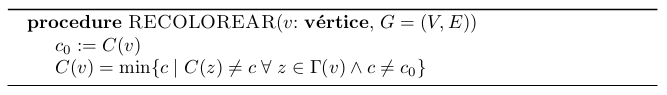
\includegraphics{definitions/algo_recolorear.png}
        \end{adjustbox}
    

Esta función cambia el color del vértice $v$ tomando el mínimo color disponible (teniendo en cuenta los colores asignados a los vecinos de $v$).


    \begin{adjustbox}{max size={\textwidth}{\textheight}}
        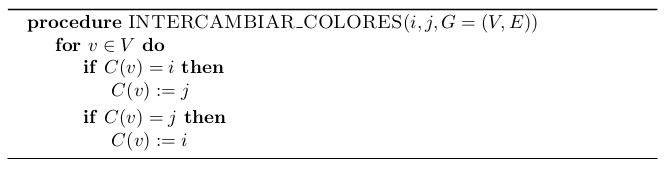
\includegraphics{definitions/alg_interc.png}
        \end{adjustbox}
    

Esta función cambia la asignación de todos los vértices que tienen el color $i$ por el color $j$ y viceversa.

\textbf{Notación}

Si $W \subseteq V$ (es decir, un subconjunto de los vértices), el subgrafo de $G$ que es generado por $W$, denotado $G[W]$ es

\begin{center}
$G[W] = (W, \{\{x, y\} \in E \mid x, y \in W\})$
\end{center}

Por ejemplo, si tomamos el grafo $G = (\{a, b, c, d\}, \{\{a, b\},\{a, c\},\{a, d\},\{b,c\}, \{b, d\}\})$ y definimos $W = \{a, d, b\}$, entonces $G[W] = (\{a, b, d\}, \{\{a, b\},\{a, d\}, \{b, d\}\})$.

\begin{center}

    \begin{adjustbox}{max size={\textwidth}{\textheight}}
        \includegraphics[width=3cm]{/tmp/tmp1OjFsF-1.png}
        \end{adjustbox}
    
    \begin{adjustbox}{max size={\textwidth}{\textheight}}
        \includegraphics[width=3cm]{/tmp/tmp1OjFsF-0.png}
        \end{adjustbox}
    
\end{center}

\begin{center}
 
\end{center}

También utilizaremos la notación $H_{i, j}$ para referirnos al subgrafo de $G$ generado por los vértices de color $i, j$ (cadena de Kempe). La idea es utilizar $\text{INTERCAMBIAR_COLORES}(i, j, K)$ sólo cuando $K$ sea una componente conexa de $H_{i,j}$.

 

\begin{center}

    \begin{adjustbox}{max size={\textwidth}{\textheight}}
        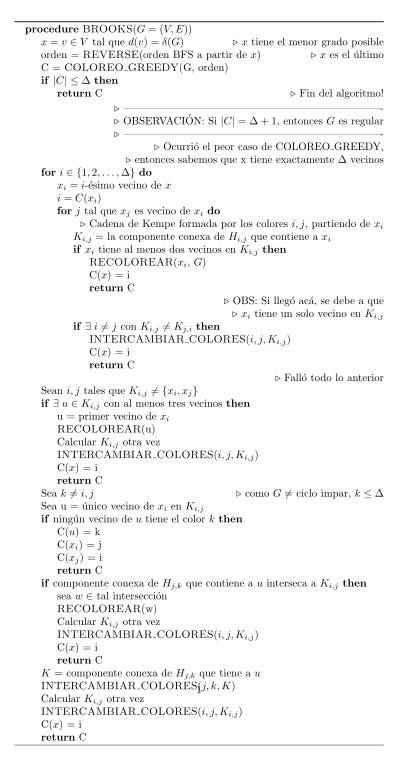
\includegraphics{definitions/algo_brooks.png}
        \end{adjustbox}
    
\end{center}

 

\section*{Greedy no siempre obtiene $\chi(G)$}

Si consideramos el grafo $G$

\begin{center}

    \begin{adjustbox}{max size={\textwidth}{\textheight}}
        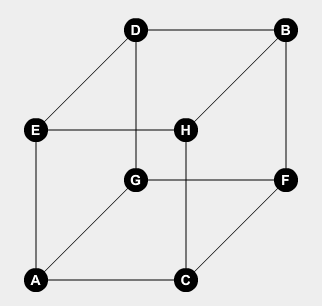
\includegraphics{definitions/graph_no_greedy.png}
        \end{adjustbox}
    
\end{center}

y corremos el algoritmo greedy en órden alfabético, obtenemos

\begin{itemize}

	\item Color de A: 1
	\item Color de B: 1
	\item Color de C: 2
	\item Color de D: 2
	\item Color de E: 3
	\item Color de F: 3
	\item Color de G: 4
	\item Color de H: 4
\end{itemize}

 

Si en cabmio corremos el algoritmo de coloreo greedy con el orden $\{A, C, H, E, D, G, F, B\}$ (es decir, los cuatro vértices de la "cara frontal" seguidos de los cuatro vértices de la "cara trasera", obtenemos:

\begin{itemize}

	\item Color de A: 1
	\item Color de C: 2
	\item Color de H: 1
	\item Color de E: 2
	\item Color de D: 1
	\item Color de G: 2
	\item Color de F: 1
	\item Color de B: 2
\end{itemize}

No podemos probar los $n!$ órdenes posibles de los grafos para correr el algoritmo voraz, pero existen ciertas heurísticas para ordenar los vértices de modo de (quizás) obtener un coloreo propio con menos colores que uno que ya se tiene.

 

\section*{Greedy con un orden seleccionado}

Sea $G$ un grafo y $C$ un coloreo propio cualquiera de $G$ con $k$ colores $\{1, 2, \dots, k\}$.

\begin{itemize}

	\item Reordenemos los colores con un orden \textbf{arbitrario} $(j_1, j_2, \dots, j_k)$.
	\item Ahora reordenemos los vértices poniendo primero todos los vértices del color $j_1$, luego todos los vértices del color $j_2$, así sucesivamente, hasta poner por último todos los vértices del color $j_k$.
	\item Entonces el algoritmo de coloreo greedy con ese orden colorea $G$ con a lo sumo $k$ colores.
\end{itemize}

\textbf{Prueba}

Supongamos que el teorema es verdadero para $k$ colores y probémoslo para $k + 1$.

Sea $W$ el conjunto formado por los vértices de color $j_1, j_2, \dots, j_k$, y sea $U$ el conjunto formado por los vértices de color $j_{k+1}$.

Sea $H = G[W]$ (el subgrafo de $G$ generado por $W$). Entonces $C/H$ ("$C$ restringido $H$") colorea $H$ con $k$ colores. Por hipótesis inductiva, greedy no usará más de $k$ colores para colorear $G[W]$. Digamos que usa $l$ colores, con $l \leq k$.

Ahora bien, al correr el algoritmo greedy sobre el grafo $G$ (ahora sí el grafo entero, no sólo $G[W]$) va a hacer lo mismo hasta terminar de colorear todos los vértices de $H$ (es decir, $W)$: va a colorear todos los vértices que están en $W$ usando sólo $l$ colores. Nos preguntamos entonces, ¿cuántos colores extra necesitará greedy para los vértices de $U$?

Si $x \in U$:

\begin{enumerate}

	\item si $\exists \;j \leq l : x$ "no es vecino de ningún vértices de color $j$", greedy no requiere ningún color extra
	\item si no, greedy le dará el color extra $l + 1$
\end{enumerate}

Es decir, el algoritmo greedy no e puede ver forzado a dar un color $l + 2$, porque para que pase eso, necesariamente $x$ tiene que ser vecino de otro vértice de color $l + 1$. Los únicos vértices que tienen color $l + 1$ son los de $U$, que no forman vértices por definición (todos tienen el color $j_{k+1}$.

Por lo tanto, greedy va a utilizar a los sumo $l + 1$ colores.

\textbf{Corolario}

Existe un orden $\leq$ de los vértices tal que greedy $(G, \leq) = \chi(G)$.

\textbf{Prueba}

Sea $C$ un coloreo propio con $\chi(G)$ colores. Entonces greedy en el orden de los vértices dado por este coloreo produce un coloreo $C'$ con a lo sumo $\chi(G)$ colores. Como $\chi(G)$ es el mínimo, greedy on ese orden utiliza $\chi(G)$ colores.

\section*{Baby Brooks}

Sea $G$ un grafo conexo no regular, entonces $\chi(G) \leq \Delta(G)$

Notemos que este teorema es más débil que el Teorema general de Brooks, ya que este no afirma nada en relación a los ciclos pares, mientras que aquel sí.

\textbf{Prueba}

\begin{enumerate}

	\item Elegir $x$ con $d(x) = \delta(G)$ (un vértice de menor grado posible).
	\item Ordenar los vértices con el orden inverso al dado por BFS(x), es decir, $x_1, x_2, \dots, x_{n-1}, x_n = x$
	\item Correr el algoritmo greedy en ese orden
\end{enumerate}

\vspace{0.5cm}\hrule\vspace{0.5cm}
\textbf{Afirmación}

Si $i\leq n-1$ greedy colorea $x_i$ con algún color en $\{1, 2, \dots, \Delta(G)\}$

\textbf{Subprueba}

El vértice $x_i$ fue "puesto" en el orden BFS por algún vecino. El único que no fue puesto por ningún vecino fue el propio $x_n = x$, que por la definición de $i$ queda excluido de esta afirmación. Por lo tanto este vecino (el que incluyó a $x_i$) estaba antes en el orden BFS. Sin embargo, como estamos usando el orden BFS invertido, ahora está después.

Pero por la forma en que funciona BFS, ese "alguien" es sí o sí vecino de $x_i$. En consecuencia, podemos asegurar que para todo $x_i$ hay un $x_j$ (con $j > i$) que es vecino de $x_i$ en el grafo.

Ahora bien:

\begin{enumerate}

	\item $\forall \; i \leq n-1$, $\exists\;j>i:x_j \in \Gamma(x_i)$
	\item $\forall \; i \leq n-1$, cuando vamos a colorear $x_i$, existe algún vecino de $x_i$ sin colorear (porque $x_j$ está después y todavía no llegué a colorearlo).
\end{enumerate}

Por lo tanto, el número de vecinos coloreados de $x_i$ es a lo sumo $d(x_i) -1$ y $d(x_i) \leq \Delta(G)$ (aclaración: en los apuntes tengo $d(x_i) \leq \Delta(G) -1$, pero me parece incorrecto), por lo tanto greedy elimina a los sumo $\Delta(G) - 1$ colores, y seguro que le da a $x_i$ algún color en $\{1,2,\dots, \Delta(G)\}$.

\textbf{(Fin supbrueba)}

\vspace{0.5cm}\hrule\vspace{0.5cm}
Hemos probado la afirmación sin usar que $G$ no es regular. Queda aún por colorear $x_n$. Para $x_n=x$ todos sus vecinos están ya coloreados. Greedy puede eliminar a lo sumo $d(x)$ colores. Pero $d(x) = \delta(G)$ y como $G$ no es regular, se tiene  $\delta(G) < \Delta(G)$. Luego, greedy elimina $\delta(G)<\Delta(G)$ colores y colorea $x$ con algún color en $\{1, 2, \dots, \Delta(G)\}$.

\section*{Grafo dirigido}

Un grafo dirigido es un par $(V, E)$ con $E \subseteq V \times V$ (son pares ordenados).

\section*{Network}

Un Network es una $5$-tupla $N = (V, E, C, s, t)$ tal que

\begin{enumerate}

	\item $(V, E)$ es un grafo dirigido
	\item $C$ es una función $E \rightarrow \mathbb{R}_{\geq0} \cup \infty$ (función "capacidad")
	\item $s, t \in V$ tales que no exista $v\in V$ con $(v, s) \in E$ o $(t,v)\in E$.
\end{enumerate}

$s$ (source) sólo es vértice de partida de cualquier lado ("no consume"), mientras que $t$ (sink) es sólo vértice de llegada ("no produce").

\textbf{Notación}

\begin{itemize}

	\item \textbf{$\overrightarrow{xy}$ }denota al lado $(x, y)$
	\item $\Gamma^+(x) = \{y \in V: \overrightarrow{xy} \in E\}$ (el conjunto de vértices a los cuales se puede ir desde $x$)
	\item $\Gamma^-(x) = \{y \in V: \overrightarrow{yx} \in E\}$ (el conjunto de vértices desde los cuales se puede llegar a $x$)
\end{itemize}

 

\section*{Flujo}

Un flujo en un network $N$ es una función $f: E \rightarrow R_{\geq 0}$ tal que

\begin{enumerate}

	\item $0 \leq f(\overrightarrow{xy})\leq C(\overrightarrow{xy})$ ("Feasability")
	\item Para todo $x \neq s, t$, $\sum\limits_{y\,\in\,\Gamma^+(x)} f(\overrightarrow{xy}) = \sum\limits_{y\,\in\,\Gamma^-(x)} f(\overrightarrow{xy})$ (todo lo que entra debe salir)
\end{enumerate}

\section*{Valor de un flujo}

El valor de un flujo $f$ en un network $N$, denotado $v(f)$ es

\begin{center}
$v(f) = \sum\limits_{z\,\in\,\Gamma(s)}f(\overrightarrow{sz})$
\end{center}

\section*{Flujo entero}

Un flujo $f$ en un network $N$ se dice \textbf{entero} si

\begin{center}
$f(\overrightarrow{xy}) \in \mathbb{Z} \;\forall\;\overrightarrow{xy} \in E$
\end{center}

\begin{center}
 
\end{center}

\section*{Flujo entero maximal}

Un flujo entero maximal es un flujo entero tal que $v(f)$ es máximo entre todos los flujos enteros.

\section*{Operadores cuantificados sobre subconjuntos de $V$}

Dado un grafo $G$, sean $A, B \subseteq V$ y sea $\phi: E\rightarrow \mathbb{R}$ una función que asocia un número real a un lado del grafo $G$. Entonces adoptamos la notación $\phi(A, B)$ para denotar la sumatoria de los valores que toma $\phi$ para todos aquellos lados del grafo que comienzan en $A$ y terminan en $B$:

\begin{center}
$\Phi(A, B) = \sum\limits_{\substack{x \in A\\ y \in B \\ \overrightarrow{xy} \in E}}\phi(\overrightarrow{xy})$
\end{center}

Además, si $x \in V$, como una extensión a esta notación, podemos escribir:

\begin{center}
$\phi (x, B) = \phi(\{x\}, B)$
\end{center}

\begin{center}
$\phi (A, x) = \phi(A, \{x\})$
\end{center}

Como ejemplos:

\begin{itemize}

	\item $f(A, B)$ es la sumatoria del flujo $f$ en lados que empiezan en $A$ y terminan en $B$.
	\item $CAP(A, B)$ es la capacidad de los lados que empiezan en $A$ y terminan en $B$
	\item $OUT_f(x) = f(x, V)$
	\item $IN_f(x) = f(V, x)$
\end{itemize}

\section*{Relacion entre $v(f)$, el flujo saliente de $s$ y el flujo entrante a $t$}

\begin{center}
$v(f) = OUT_f(s) = IN_f(t)$
\end{center}

\textbf{Prueba}

Por definición, $v(f) = \sum\limits_{z\,\in\,\Gamma(s)}f(\overrightarrow{xy})$, es decir, $v(f) = OUT_f(s)$. Veamos entonces la segunda igualdad.

Si tomamos la fórmula:

\begin{center}
\begin{align*} f(V, V) &= \sum\limits_{\substack{x, y\, \in\, V\\\overrightarrow{xy}\, \in \,E}} f(\overrightarrow{xy})\\ &= \sum\limits_{x\, \in\, V} \left(\sum\limits_{\substack{ y\, \in\, V\\\overrightarrow{xy}\, \in \,E}} f(\overrightarrow{xy})\right)\\ &= \sum\limits_{x\, \in\, V} f(x, V) \\ &= \sum\limits_{x\, \in\, V}OUT_f(x) \end{align*}
\end{center}

Pero también podemos escribir

\begin{center}
\begin{align*} f(V, V) &= \sum\limits_{\substack{x, y\, \in\, V\\\overrightarrow{yx}\, \in \,E}} f(\overrightarrow{yx})\\ &= \sum\limits_{x\, \in\, V} \left(\sum\limits_{\substack{ y\, \in\, V\\\overrightarrow{yx}\, \in \,E}} f(\overrightarrow{yx})\right)\\ &= \sum\limits_{x\, \in\, V} f(V, x) \\ &= \sum\limits_{x\, \in\, V}IN_f(x) \end{align*}
\end{center}

Entonces,

\begin{center}
$\sum\limits_{x \in V} OUT_f(x) = \sum\limits_{x \in V}IN_f(x)$
\end{center}

Si reescribimos esta fórmula haciendo un poco más explícitos sus términos:

\begin{center}
\begin{align*} \sum\limits_{x \in V} OUT_f(x) &= OUT_f (x_1) + OUT_f(x_2) + \dots + OUT_f(x_n) \\ &= IN_f (x_1) + IN_f(x_2) + \dots + IN_f(x_n)\\ &= \sum\limits_{x \in V}IN_f(x) \end{align*}
\end{center}

Pero si $OUT_f(x) = IN_f(x)$ para todo $x \neq s, t$, sólo quedan los términos:

\begin{center}
$OUT_f(s) + OUT_f(t) = IN_f(s) + IN_f(t)$
\end{center}

Sin embargo, no existen lados $\overrightarrow{xs}$ ni $\overrightarrow{tx}$, por lo tanto

\begin{center}
$IN_f(s) = OUT_f(t) = 0 $
\end{center}

En consecuencia:

\begin{center}
$OUT_f(s) = IN_f(s)$
\end{center}

\section*{Corte}

Dado un network $N=(V, E, C, s, t)$, un subconjunto $S \subset V$ se dice corte si

\begin{enumerate}

	\item $s\in S$
	\item $t\not \in S$
\end{enumerate}

Ejemplos de cortes:

\begin{itemize}

	\item $S_1 = \{s\}$
	\item $S_2 = V - \{t\}$
\end{itemize}

\section*{Capacidad de un corte}

Dado un network $N$, la capacidad de un corte $S$ es

\begin{center}
\begin{align*} CAP(S) &= c(S, V-S)\\ &= \sum\limits_{\substack{x\,\in\,S \\ y \,\not \in\,S\\ \overrightarrow{xy}\in E }} c(\overrightarrow{xy} ) \end{align*} 
\end{center}

Ejemplo:

\begin{center}

    \begin{adjustbox}{max size={\textwidth}{\textheight}}
        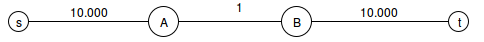
\includegraphics{definitions/cut.png}
        \end{adjustbox}
    
\end{center}

\begin{itemize}

	\item $CAP(\{s\}) = c(\overrightarrow{sA}) = 10.000$
	\item $CAP(\{s, A\}) = c(\overrightarrow{AB}) = 1$
\end{itemize}

 

\section*{Camino aumentante}

Dado un network $N = (V, E, C, s, t)$, un "camino aumentante" (augmenting path) es una sucesión de vértices $x_0 = s, x_1, x_2, \dots, x_r = t$ tales que para todo $0\leq i < r$ se cumple que una de estas dos cosas:

\begin{itemize}

	\item $\overrightarrow{x_ix_{i+1}} \in E$ (es lado "forward") y $f(\overrightarrow{x_ix_{i+1}}) < c(\overrightarrow{x_ix_{i+1}})$ (se puede aún mandar más flujo), o bien
	\item $\overrightarrow{x_{i+1}x_i} \in E$ (es lado "backwards") y $f(\overrightarrow{x_{i+1}x_i}) > 0$ (se puede aún "devolver" flujo al anterior.
\end{itemize}

\section*{Generalización de $v(f)$}

Sea $S$ un corte y $f$ un flujo, entonces

\begin{center}
$v(f) = f(S, V- S) - f(V-S, S)$
\end{center}

Esta idea generaliza la noción de $v(f)$ para conjuntos.

\textbf{Prueba}

Sea $x \in S$. En particular $x\neq t$ (ya que $S$ es corte). Entonces

\begin{center}
$f(x, V) - f(V, x) = \begin{cases} 0 & x\neq s\\ v(f) &x=s \end{cases}$
\end{center}

Entonces

\begin{center}
\begin{align*} v(f) &= v(f) + 0 + 0 + \dots\\ &= \sum\limits_{x\,\in\, S} \left(f(x, V) - f(V, x)\right)\\ &= f(S, V) - f(V, S)\\ \end{align*}
\end{center}

Si ahora partimos $V$ en dos subconjuntos disjuntos: $V - S$ y $S$, podemos continuar

\begin{center}
\begin{align*} f(S, V) - f(V, S) &= f(S, S) + f(S, V-S) - f(S, S) - f(V-S, S)\\ &= f(S, V-S) - f(V-S, S)\\ \end{align*}
\end{center}

\section*{Flujo a partir de un camino aumentante}

Dado un network $N = (V, E, C, s, t)$ y un flujo $f$ sobre $N$. Sea además $x_0 = s, x_1, x_2,\dots, x_r=t$ un camino aumentante entre $s$ y $t$. Sea

\begin{center}
$\epsilon_i = \begin{cases} c(\overrightarrow{x_ix_{i+1}}) - f(\overrightarrow{x_ix_{i+1}}) & \text{ si } \overrightarrow{x_ix_{i+1}} \text{ es lado forward}\\ f(\overrightarrow{x_{i+1}x_i}) &\text{ si } \overrightarrow{x_ix_{i+1}} \text{ es lado backwards} \end{cases}$
\end{center}

Notemos que $\epsilon_i$ es "lo que podría aumentar" si estoy considerando un lado forward, o lo que me podrían devolver, si estoy considerando un lado backwards.

Sea $\varepsilon = \min(\epsilon_i)$ (que debe ser positivo por tener un camino aumentante.

Sea $f^*$ una función sobre los lados del network

\begin{center}
$f^*(\overrightarrow{x_ix_{i+1}}) = \begin{cases} f(\overrightarrow{x_ix_{i+1}}) + \varepsilon & \text{ si }\overrightarrow{x_ix_{i+1}} \text{ es un lado forward}\\ f(\overrightarrow{x_ix_{i+1}}) - \varepsilon & \text{ si }\overrightarrow{x_ix_{i+1}} \text{ es un lado backward}\\ \end{cases} $
\end{center}

y además

\begin{center}
$f^*(\overrightarrow{xy}) = f(\overrightarrow{xy})$
\end{center}

para todos los otros lados.

Entonces $f^*$ es flujo y $v(f^*) = v(f)+\varepsilon$

\textbf{Prueba}

La prueba tiene la siguiente estructura

\begin{enumerate}

	\item Probar que $0 \leq f^* (v)$
	\item Probar que $f^* \leq c$
	\item Conservación: $f^*(x, V) = f^*(V, x) \quad\forall\; x\neq s, t$
	\item Probar que $v(f^*) = v(f)+\varepsilon$
\end{enumerate}

1) $0 \leq f^* (v)$

En los lados "forward" del camino aumentante (aquellos que pertenecen a $E$ en los que aún puedo aumentar la capacidad), $f^*$ está definida como

\begin{center}
$f^*(\overrightarrow{x_ix_{i+1}}) = f(\overrightarrow{x_ix_{i+1}})+\varepsilon \geq \varepsilon \geq 0 $
\end{center}

Mientras que en los lados "backwards" (aquellos que invertidos pertenecen a E, pero aún puedo devolver flujo) está definido como

\begin{center}
$f^*(\overrightarrow{x_{i+1}x_{i}}) = f(\overrightarrow{x_{i+1}x_{i}}) - \varepsilon \geq f(\overrightarrow{x_{i+1}x_{i}}) -\epsilon_i = 0$
\end{center}

2) $f^* \leq c$

En los lados "backwards", esto es obvio, porque $f$ es un flujo y estoy restando del mismo, por lo que sigue siendo $f^* = f - \varepsilon < f \leq c $

En los lados "forward"

\begin{center}
\begin{align*} f^*(\overrightarrow{x_ix_{i+1}}) &= f(\overrightarrow{x_ix_{i+1}}) + \varepsilon\\ &\leq f(\overrightarrow{x_ix_{i+1}}) + \epsilon_i\\ &= f(\overrightarrow{x_ix_{i+1}})+c(\overrightarrow{x_ix_{i+1}})-f(\overrightarrow{x_ix_{i+1}})\\ &= c(\overrightarrow{x_ix_{i+1}}) \end{align*}
\end{center}

3) $f^*(x, V) = f^*(V, x) \quad\forall\; x\neq s, t$

Si $x$ no es uno de los $x_i$ (esto es, no forma parte del camino aumentante) el valor del flujo entrante y saliente viene dado por $f$, por lo que la conservación está asegurada.

Si, en cambio, $x$ es parte del camino aumentante, es decir $x = x_i$ con $1 \leq i \leq r-1$ (pues $x \neq s, t$), entones existen $x_{i-1}$ y $x_{i+1}$ (es decir, hay un lado entrante y un lado saliente de $x_i$).

\begin{center}

    \begin{adjustbox}{max size={\textwidth}{\textheight}}
        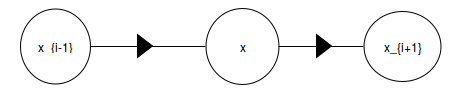
\includegraphics{definitions/f_estrella_1.jpg}
        \end{adjustbox}
    
\end{center}

Como no sabemos si se trata de lados forward o lados backwards, debemos analizar cuatro casos.

\textbf{CASO 1}: tanto $\overrightarrow{x_{i-1}x_{i}}$ como  $\overrightarrow{x_{i}x_{i+1}}$ son lados forward:

\begin{center}

    \begin{adjustbox}{max size={\textwidth}{\textheight}}
        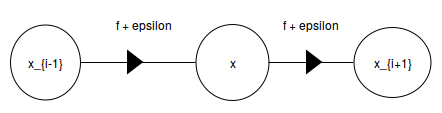
\includegraphics{definitions/f_estrella_2.png}
        \end{adjustbox}
    
\end{center}

Entonces

\begin{center}
$f^*(x_i, V) = f(x_i, V) + \varepsilon$ (a causa del lado $\overrightarrow{x_{i}x_{i+1}}$)
\end{center}

\begin{center}
$f^*(V, x_i) = f(V, x_i) + \varepsilon$ (a causa del lado $\overrightarrow{x_{i-1}x_{i}}$)
\end{center}

Como $f$ es flujo, se tiene que $f(x_i, V) = f(V, x_i)$, por lo tanto $f^*$ mantiene la conservación en este caso.

\textbf{CASO 2}: tanto $\overleftarrow{x_{i-1}x_{i}}$ como  $\overleftarrow{x_{i}x_{i+1}}$ son lados backwards, esto quiere decir que verán decrementado el flujo en $\varepsilon$.

\begin{center}

    \begin{adjustbox}{max size={\textwidth}{\textheight}}
        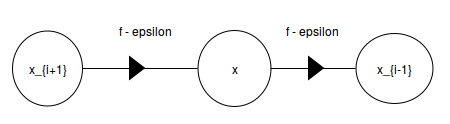
\includegraphics{definitions/f_estrella_3.png}
        \end{adjustbox}
    
\end{center}

\begin{center}
$f^*(x_i, V) = f(x_i, V) - \varepsilon$ (a causa del lado $\overrightarrow{x_{i}x_{i-1}}$)
\end{center}

\begin{center}
$f^*(V, x_i) = f(V,x_i) - \varepsilon$ (a causa del lado $\overrightarrow{x_{i+1}x_i}$)
\end{center}

Por un razonamiento análogo al caso anterior, se ve que $f^*$ también cumple la conservación en este caso.

\textbf{CASO 3}: $\overrightarrow{x_{i-1}x_{i}}$ es un lado forward (es un lado del network que verá incrementado su flujo en $\varepsilon$), pero $\overleftarrow{x_{i}x_{i+1}}$ es un lado backwards que verá decrementado su flujo en $\varepsilon$. Es decir, en el grafo se producirá:

\begin{center}

    \begin{adjustbox}{max size={\textwidth}{\textheight}}
        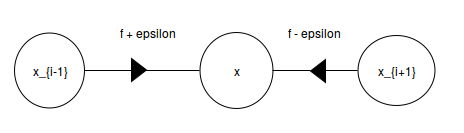
\includegraphics{definitions/f_estrella_4.png}
        \end{adjustbox}
    
\end{center}

Notemos que en el camino aumentante, $x_{i+1}$ es posterior a $x_i$ pero es un lado backwards, o sea que en el grafo, existe el lado $\overrightarrow{x_{i+1}x_{i}}$ (tanto $x_{i-1}$ como $x_{i+1}$ están en $\Gamma^-(x_i))$. En este caso

\begin{center}
$f^*(x_i, V) = f(x_i, V)$
\end{center}

pues no hay lados que salgan de $x_i$ que hayan cambiado su flujo. En cuanto al flujo entrante:

\begin{center}
$f^*(V, x_i) = f(V, x_i) + \varepsilon - \varepsilon = f(V, x_i)$
\end{center}

Luego, se mantiene la conservación en este caso.

\textbf{CASO 4}: $\overleftarrow{x_{i-1}x_{i}}$ es un lado backwards (es decir, $\overrightarrow{x_{i}x_{i-1}}$ un lado del network que verá decrementado su flujo en $\varepsilon$), pero $\overrightarrow{x_{i}x_{i+1}}$ es un lado forward que verá incrementado su flujo en $\varepsilon$. Es decir, en el grafo se producirá:

\begin{center}

    \begin{adjustbox}{max size={\textwidth}{\textheight}}
        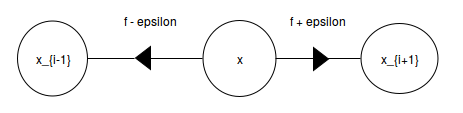
\includegraphics{definitions/f_estrella_5.png}
        \end{adjustbox}
    
\end{center}

Notemos que en el camino aumentante, $x_{i-1}$ es anterior a $x_i$ pero es un lado backwards, o sea que en el grafo, existe el lado $\overrightarrow{x_{i}x_{i-1}}$ (tanto $x_{i-1}$ como $x_{i+1}$ están en $\Gamma^+(x_i)$). En este caso

\begin{center}
$f^*(V, x_i) = f(V, x_i)$
\end{center}

pues no hay lados que entren a $x_i$ que hayan cambiado su flujo. En cuanto al flujo saliente:

\begin{center}
$f^*(x_i, V) = f(x_i, V) + \varepsilon - \varepsilon = f(x_i, V)$
\end{center}

Luego, se mantiene la conservación en este caso.

Hemos probado que $f^*$ es flujo. Falta ver la segunda afirmación

4) $v(f^*) = v(f)+\varepsilon$

Para todos los lados vértices vecinos de $s$ que no formaban parte del camino aumentante, el valor de $f^*$ es igual al valor de $f$. Sin embargo, hay un único vértice $x_1$ que formaba parte del camino aumentante, por lo tanto:

\begin{center}
$v(f^*) = f^*(s, V) = f(s, V) + \varepsilon $
\end{center}

\section*{Max flow, min cut}

Sea un network $N = (V, E, c, s, t)$.

\begin{enumerate}

	\item Si $f$ es flujo y $S$ es corte, entonces $v(f) \leq CAP(S) $
	\item Si $v(f) = CAP(S)$, entonces $f$ es maximal y $S$, minimal
	\item Si $f$ es maximal, entonces existe un corte $S$ con $v(f) = CAP(S)$
\end{enumerate}

\textbf{Prueba}

1)

\begin{center}
\begin{align*} v(f) &= f(S, V - S) - f(V-S, S)\\ &\leq f(S, V - S) \\ &\leq c(S, V - S)\\ &= CAP(S) \end{align*}
\end{center}

2)

Spongamos $v(f) = CAP(S)$. Sea $g$ cualquier flujo, por 1) se tiene que

\begin{center}
\begin{align*} v(g) &\leq CAP(S)\\ &= v(f) \end{align*}
\end{center}

es decir, $f$ es maximal. Por otro lado, sea $T$ un corte. Entonces por 1) se tiene que

\begin{center}
\begin{align*} CAP(T) &\geq v(f)\\& = CAP(S) \end{align*}
\end{center}

es decir, $S$ es minimal.

3)

Sea $S =\{s\}\cup\{x: \text{ existe un camino aumentante (relativo a } f \text{)}\text{ entre }s \text{ y } x \}$ un candidato a corte. Nos hacemos la pregunta:

¿Está $t$ en $S$? Si suponemos que sí, entonces existe un camino aumentante entre $s$ y $t$, por la propiedad demostrada anteriormente (ver aquí) debemos aceptar que existe un flujo $f^*$ y $\varepsilon > 0$ con $v(f^*) = v(f) + \varepsilon$, lo cual es absurdo. Por lo tanto, $t$ no está en $S$. Esto implica que $S$ es corte. Calculemos su capacidad.

Tenemos que

\begin{center}
$v(f) = f(S, V- S)-f(V-S, S)$
\end{center}

Analicemos cada término:

\begin{center}
$f(S, V- S) = \sum\limits_{\substack{x \,\in \, S\\z \,\in\,V-S\\ \overrightarrow{xz} \,\in\,E}}f(\overrightarrow{xz})$
\end{center}

Como $x \in S$ entonces existe un camino aumentante entre $s$ y $x$ y como $z\not \in S$, entonces no existe un camino aumentante entre $s$ y $z$. Entonces si $\overrightarrow{xz} \in E$, $f(\overrightarrow{xz}) = c(\overrightarrow{xz})$ (el flujo enviado iguala a la capacidad, ya no se puede enviar más). Por lo tanto,

\begin{center}
\begin{align*} f(S, V- S) &= \sum\limits_{\substack{x \,\in \, S\\z \,\in\,V-S\\ \overrightarrow{xz} \,\in\,E}}f(\overrightarrow{xz})\\ &= \sum\limits_{\substack{x \,\in \, S\\z \,\in\,V-S\\ \overrightarrow{xz} \,\in\,E}}c(\overrightarrow{xz})\\ &= c(S, V-S)\\ &= CAP(S) \end{align*}
\end{center}

Por otro lado,

\begin{center}
\begin{align*} f(V, S-V) &= \sum\limits_{\substack{x\,\in\,V -S\\ z \,\in\,S\\ \overrightarrow{xz} \,\in\,E}}f(\overrightarrow{xz})\\ \end{align*}
\end{center}

Si $x\in V - S$ entonces no existe camino aumentante entre $s$ y $x$. Si $z\in S$ entonces existe un camino aumentante $s=z_0, z_1, \dots, z_r=z$. En particular, $s=z_0, z_1, z_2,\dots, z_r=z, x$ no es un camino aumentante, entonces $f(\overrightarrow{xz}) = 0$. Luego,

\begin{center}
\begin{align*} f(V, S-V) &= \sum\limits_{\substack{x\,\in\,V -S\\ z \,\in\,S\\ \overrightarrow{xz} \,\in\,E}}f(\overrightarrow{xz})\\ &= \sum\limits_{\substack{x\,\in\,V -S\\ z \,\in\,S\\ \overrightarrow{xz} \,\in\,E}}0\\ &= 0 \end{align*}
\end{center}

Entonces, retomando el incio del inciso 3)

\begin{center}
$v(f) = f(S, V- S)-f(V-S, S) = CAP(S) - 0 = CAP(S)$
\end{center}

\section*{Ford-Fulkerson}


    \lstset{
        commentstyle=\color{mygreen},
        keywordstyle=\color{myred},
        frame=single,
        backgroundcolor=\color{gray!10},
        inputencoding=utf8,
        extendedchars=true,
        mathescape=true,
        breaklines=true,
        literate={á}{{\'a}}1 {é}{{\'e}}1 {í}{{\'i}}1 {ó}{{\'o}}1 {ú}{{\'u}}1 {ñ}{{\~n}}1
    }
    \begin{lstlisting}[language=pseudo]
procedure FORD_FULKERSON
    f = 0
    flag = True
    while flag:
        if $\exists$ camino aumentante entre $s$ y $t$:
            construir f$^*$ a partir de f como en el lema
        else:
            flag = False
\end{lstlisting}


Como consecuencia del teorema "Max flow, min cut", podemos afirmar que si el algoritmo de Ford-Fulkerson termina es porque ya no hay caminos aumentantes entre $s$ y $t$, por lo tanto existe un corte $S$ con $v(f) = CAP(S)$ y por lo tanto, el flujo es maximal.

El algoritmo, sin embargo, tiene dos problemas:

\begin{enumerate}

	\item No siempre termina
	\item Su complejidad puede ser muy mala
\end{enumerate}

\subsubsection*{Ejemplo de que Ford-Fulkerson puede no terminar}

Consideremos el siguiente network

\begin{center}

    \begin{adjustbox}{max size={\textwidth}{\textheight}}
        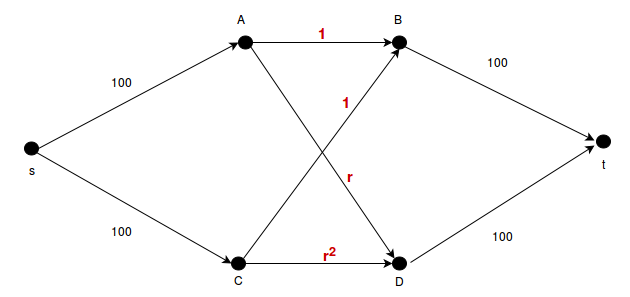
\includegraphics{definitions/ff_problem_1.png}
        \end{adjustbox}
     
\end{center}

donde $r$ es la única raíz positiva de $p(x) = x^3+x -1$.

Observación: $p(x) = x^3 + x - 1$ tiene una sola raíz positiva porque $p(0) = -1 < 0$, $p(1) = 1>0$ y la primera derivada de la función, $p' (x) = 3x^2+1$ es siempre positiva (es decir, la función es creciente, y por el toerema del valor medio toma todos los valores entre $-1$ y $1$ en el intervalo $[0, 1]$).

Observación: Como $p(0) < 0 < p(1)$, se tiene que $r \in (0, 1)$ y por lo tanto, $1 > r > r^2 > r^3 > \dots$

El algoritmo de Ford-Fulkerson podría tomar los siguientes caminos

\textbf{Camino 0: }$sABt$ con $\varepsilon = 1$, $v(f_0) = 1$


    \begin{adjustbox}{max size={\textwidth}{\textheight}}
        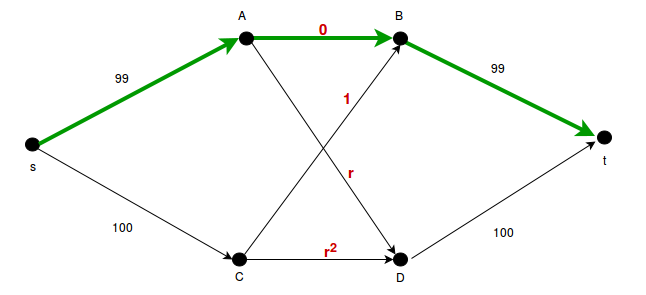
\includegraphics{definitions/ff_problema_1b.png}
        \end{adjustbox}
    

\begin{itemize}

	\item $(c_0 - f_0) (\overrightarrow{AB}) = 0$
	\item $(c_0 - f_0) (\overrightarrow{CB}) = 1 = r^0$
	\item $(c_0 - f_0) (\overrightarrow{AD}) = r = r^1$
	\item $(c_0 - f_0) (\overrightarrow{CD}) = r^2$
\end{itemize}

Llamemos $\psi_0$ al conjunto formado por estos cuatro valores:

\begin{center}
$\psi_0 = \{ (c_0-f_0)(\overrightarrow{AB}), (c_0-f_0)(\overrightarrow{CB}), (c_0-f_0)(\overrightarrow{AD}), (c_0-f_0)(\overrightarrow{CD})\} = \{0, 1, r, r^2\}$
\end{center}

\textbf{Camino 1: }$sC\overleftarrow{BA}Dt$ con $\varepsilon = r$, y $v(f_1) = 1 + r$


    \begin{adjustbox}{max size={\textwidth}{\textheight}}
        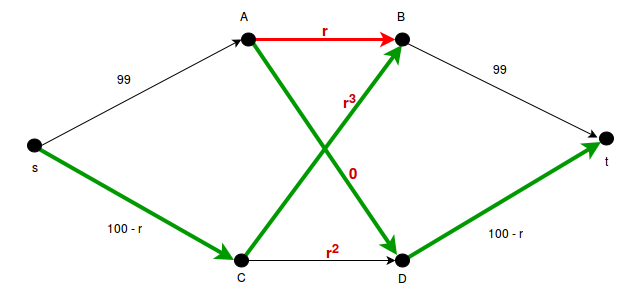
\includegraphics{definitions/ff_problema_1c.png}
        \end{adjustbox}
    

\begin{itemize}

	\item $(c_1 - f_1) (\overrightarrow{AB}) = 1 - (1-r) = r$
	\item $(c_1 - f_1) (\overrightarrow{CB}) = 1- r = r^3$
	\item $(c_1 - f_1) (\overrightarrow{AD}) = r - r=0$
	\item $(c_1 - f_1) (\overrightarrow{CD}) = r^2 - 0 = r^2$
\end{itemize}

El conjunto formado por estos cuatro valores es

\begin{center}
$\psi_1 = \{(c_1-f_1)(\overrightarrow{AB}), (c_1-f_1)(\overrightarrow{CB}), (c_1-f_1)(\overrightarrow{AD}), (c_1-f_1)(\overrightarrow{CD})\} = \{r, r^3, 0, r^2\}$
\end{center}

Parece haber un patrón, que intentaremos probar por inducción.

\subsubsection*{\textbf{Hipótesis Inductiva:}}

\textbf{Camino $j$:}

Sin tener en cuenta el orden de los elementos del conjunto, para $j \in \mathbb{N}$ se cumple que $\psi_j= \{0, r^j, r^{j+1}, r^{j+2}\}$

y

si $\overrightarrow{h_je_j}$ es el lado que cumple $(c_j-f_j)(\overrightarrow{h_je_j}) = 0$

si $\overrightarrow{g_jd_j}$ es el lado que cumple $(c_j-f_j)(\overrightarrow{g_jd_j}) = r^{j+2}$

entonces $\{h_j, e_j\}\cap \{g_j, d_j\} = \emptyset$

\subsubsection*{\textbf{Prueba:}}

Notemos que los vértices nomenclados $h_j$ y $g_j$ son "anteriores" en el grafo a los nomenclados $e_j$ y $d_j$ (en el gráfico, $h_j$ y $g_j$ pueden ser $A$ ó $C$, mientras que $e_j$ y $d_j$ corresponden a $B$ ó $D$).

\textbf{Camino $j+1$}: $sg_j\overleftarrow{e_jh_j}d_jt$ con $\varepsilon = r^{j+1}$ y $v(f_{j+1}) = v(f_j)+r^{j+1}$

Sabemos que

\begin{itemize}

	\item por los lados $\overrightarrow{g_je_j}$ y $\overrightarrow{h_jd_j}$ el flujo se incrementa en $r^{j+1}$, por lo tanto en el ciclo anterior, tenían una capacidad residual de al menos $r^{j+1}$. De ellos, uno era el lado cuya capacidad residual era $r^j$ (y ahora es $r^j - r^{j+1} = r^j(1-r) = r^jr^3= r^{j+3}$), mientras que el otro era el lado cuya capacidad residual era $r^{j+1}$ (y ahora es $r^{j+1} - r^{j+1} = 0$).
	\item por el lado backwards $\overleftarrow{e_jh_j}$ el flujo es, en cambio, decrementado en $r^{j+1}$, por lo tanto, en el ciclo anterior mandaba al menos $r^{j+1}$ y su capacidad residual era menor que $1 - r^j+1$
	\item si tomamos $(c_{j+1}-f_{j+1})(\overrightarrow{h_je_j})=0+r^{j+1} = r^{j+1}$ y $(c_{j+1}-f_{j+1})(\overrightarrow{g_jd_j})=r^{j+2}$ (este último, el lado que no usamos en este camino), tenemos que
\end{itemize}

\begin{center}
$\psi_{j+1}= \{0, r^{j+1}, r^{j+2}, r^{j+3}\}$
\end{center}

y además se cumple que los lados cuya capacidad residual es o bien $0$ o bien $r^{(j+1) + 2} = r^{j+3}$ están dispuestos de modo que no comparten ningún vértice.

Tenemos que

\begin{itemize}

	\item el lado con capacidad residual $0$ es $\overrightarrow{g_je_j}$ y el lado con capacidad residual $r^{j+3}$ es $\overrightarrow{h_jd_j}$, o bien
	\item el lado con capacidad resiudal $0$ es $\overrightarrow{h_jd_j}$ y el lado con capacidad residual $r^{j+3}$ es $\overrightarrow{g_je_j}$ .
\end{itemize}

Esto prueba que el algoritmo de Ford-Fulkerson puede no terminar nunca, ya que eligiendo caminos de este modo, siempre se podrá elegir un camino aumentante más.

Podría pensarse que el valor del flujo tiende a alguna cota real $F$ cuando $j$ tiende a infinito y que $F$ es el valor del flujo maximal, sin embargo esto es incorrecto, ya que basta con agregar el lado $\overrightarrow{st}$ con capacidad $F + 1$ que el algoritmo de Ford-Fulkerson podría nunca elegirlo como camino aumentante y, por lo tanto, aproximarse infinitamente al valor $F$ cuando en realidad existe un flujo que es mayor y nunca será "visto" por el algoritmo. Ese caso se podría presentar en el siguiente network:

\begin{center}

    \begin{adjustbox}{max size={\textwidth}{\textheight}}
        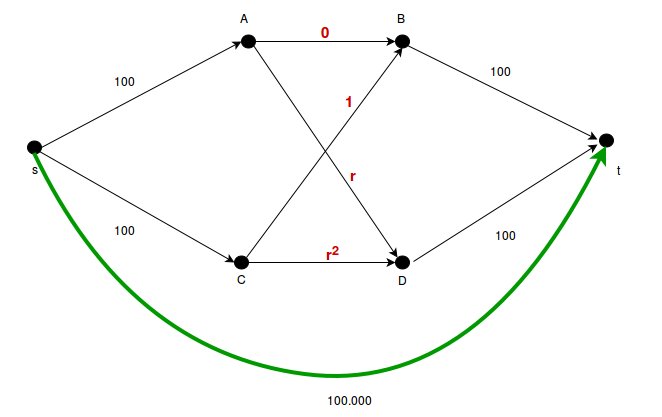
\includegraphics{definitions/ff_todo_mal.png}
        \end{adjustbox}
    
\end{center}

\subsubsection*{Ejemplo de que la complejidad de Ford-Fulkerson puede ser muy mala}

Consideremos el siguiente network

\begin{center}

    \begin{adjustbox}{max size={\textwidth}{\textheight}}
        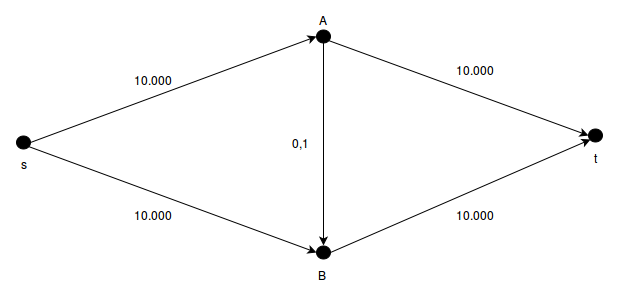
\includegraphics{definitions/ss_problem.png}
        \end{adjustbox}
    
\end{center}

Una corrida de FF podría encontrar los siguientes caminos:

\begin{itemize}

	\item $sABt$, incrementando $f$ en $0,1$
	\item $s\overleftarrow{BA}t$, incrementando $f$ en $0,1$
\end{itemize}

Repetir los dos pasos anteriores $200.000$ veces.

\section*{Teorema de la integralidad}

Sea $N = (V, E, C, s, t)$ un network. Si las capacidades de los lados son todas enteras, entonces Ford-Fulkerson termina y produce un flujo entero. En particular, si las capacidades son todas enteras, entonces existe un flujo entero maximal.

\subsubsection*{\textbf{Prueba}}

Por inducción en los flujos producidos por las sucesivas iteraciones de Ford-Fulkerson

\textbf{Caso base}

$f_0 = 0$ es entero. Sean $f_1, f_2, \dots, f_n$ los sucesivos flujos producidos por Ford-Fulkeroson.

\textbf{Hipótesis inductiva}

$f_j$ es un flujo entero

\textbf{Caso inductivo}: Si $f_j$ es entero, entonces $f_{j+1}$ es entero

$f_{j+1}$ se construye a partir de $f_j$, cambiando en algunos lados el valor $f_j$ por $f_j \pm \varepsilon$. Por lo tanto, si $\varepsilon \in \mathbb{Z}$, también se tendrá $f_{j+1} \in \mathbb{Z}$. Pero

\begin{center}
$\varepsilon = \min\{\epsilon_i\}$
\end{center}

y

\begin{center}
$\epsilon_i = \begin{cases} c(\overrightarrow{x_ix_{i+1}}) - f(\overrightarrow{x_ix_{i+1}}) & \text{ si } \overrightarrow{x_ix_{i+1}} \text{ es lado forward}\\ f(\overrightarrow{x_{i+1}x_i}) &\text{ si } \overrightarrow{x_ix_{i+1}} \text{ es lado backwards} \end{cases}$
\end{center}

Como las capacidades son todas enteras, $\epsilon_i$ es entero, $\varepsilon $ es entero y por lo tanto $f_{j+1}$ es entero.

Esto prueba que si Ford-Fulkerson termina, obtendrá un flujo maximal entero. Falta probar que efectivamente termina.

Pero $v(f_{j+1}) - v(f_j) = \varepsilon \in \mathbb{Z} > 0$, por lo tanto $\varepsilon \geq 1$. El "salto" que se produce entre un flujo y el siguiente es discreto.

Como hay una cota superior para el conjunto de valores de flujos (por ejemplo, $CAP(\{s\}) = c(s)$), esta sucesión de flujos que se incrementa en por lo menos una unidad debe acabar.

 

 

\section*{Edmonds-Karp}

Consiste en correr Ford-Fulkerson con una pequeña modificación para garantizar que el algoritmo termina. Se trata de elegir los caminos aumentantes utilizando BFS en el grafo, a partir de $s$.


    \lstset{
        commentstyle=\color{mygreen},
        keywordstyle=\color{myred},
        frame=single,
        backgroundcolor=\color{gray!10},
        inputencoding=utf8,
        extendedchars=true,
        mathescape=true,
        breaklines=true,
        literate={á}{{\'a}}1 {é}{{\'e}}1 {í}{{\'i}}1 {ó}{{\'o}}1 {ú}{{\'u}}1 {ñ}{{\~n}}1
    }
    \begin{lstlisting}[language=pseudo]
procedure EK
    // estas tres serán las variables de retorno del algoritmo

    f = 0    // El flujo maximal
    v = 0    // El valor del flujo maximal
    S = $s$  // El corte minimal

    done = false
    while Q $\neq \emptyset$:
        // Por motivos de eficiencia, conviene terminar
        // este ciclo si en la cola ya está $t$,
        // pero para calcular la complejidad de Edmond-Karp
        // no nos interesa ese aspecto
        for $z \in \Gamma^*(x) - S$
            if $f(\overrightarrow{xy}) < c(\overrightarrow{xy})$
                encolar $z$ en Q
                S = S $\cup \,\{$z$\}$
                A(z) = x    // El "ancestro" de z es x
                B(z) = 1    // Es un lado forward
                $\varepsilon(z)$ = $\min\{\varepsilon(z), c(\overrightarrow{xy}) - f(\overrightarrow{xy})\}$
        for $z \in \Gamma^-(x) - S$
            if $f(\overrightarrow{xy}) > 0$
                encolar $z$ en Q
                S = S $\cup \,\{$z$\}$
                A(z) = x    // El "ancestro" de z es x
                B(z) = -1    // Es un lado backward
                $\varepsilon(z)$ = $\min\{\varepsilon(z), f(\overrightarrow{xy})\}$
    if $t \not \in S$
        done = true
    else
        // reconstruir camino de $s$ a $t$
        $\varepsilon = \varepsilon(t)$
        v = v + $\varepsilon$
        q = t
        while $q\neq s$
            p = A(q) 
            if B(q) = 1
                $f(\overrightarrow{pq}) = f(\overrightarrow{pq}) + \varepsilon$
            else
                $f(\overrightarrow{qp}) = f(\overrightarrow{qp}) + \varepsilon$
            p = q
\end{lstlisting}

\section*{Max Flow usando Edmonds-Karp}

Consideremos el siguiente network:

\begin{center}

    \begin{adjustbox}{max size={\textwidth}{\textheight}}
        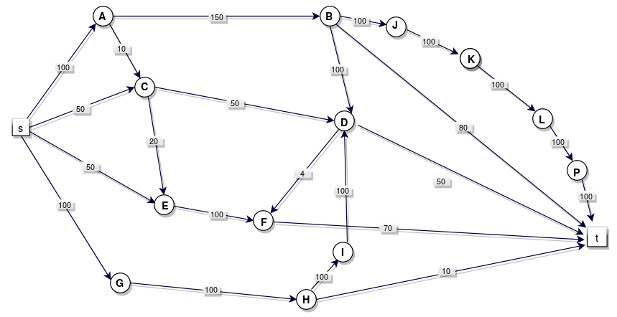
\includegraphics{definitions/EK1.jpg}
        \end{adjustbox}
    
\end{center}

Que se puede expresar como una lista de capacidades:

\begin{center}
$\begin{array}{llllll} \overrightarrow{sA}: 100& \overrightarrow{AB}: 150&\overrightarrow{BJ}: 100&\overrightarrow{DF}: 4&\overrightarrow{Ht}: 10&\overrightarrow{KL}: 100\\ \overrightarrow{sC}: 50& \overrightarrow{AC}: 10&\overrightarrow{CD}: 50&\overrightarrow{EF}: 100&\overrightarrow{HI}: 100&\overrightarrow{LP}: 100\\ \overrightarrow{sE}: 50& \overrightarrow{Bt}: 80&\overrightarrow{CE}: 20&\overrightarrow{Ft}: 70&\overrightarrow{ID}: 100&\overrightarrow{Pt}: 100\\ \overrightarrow{sG}: 100& \overrightarrow{BD}: 100&\overrightarrow{Dt}: 50&\overrightarrow{GH}: 100&\overrightarrow{JK}: 100&\\ \end{array}$
\end{center}

En cada paso, hacemos lo siguiente:

\begin{enumerate}

	\item Corremos BFS desde $s$ hasta que en la cola aparezca $t$, señalando para cada vértice que encolamos

	\begin{enumerate}

		\item quién lo incluyó en la cola
		\item cuál es el flujo máximo que puede enviar (o devolver) ese lado
	\end{enumerate}
	
	\item Cuando llegamos a $t$, calculamos $\varepsilon$ a partir del camino aumentante obtenido
	\item Actualizamos el valor de $f$.
\end{enumerate}

\subsubsection*{Paso 1}

Por ser el primer paso, se hace con mayor detalle. Después se expresa la corrida de BFS como una gran tabla.

Comenzamos por $s$, que puede incluir a $A$ (enviando $100$), a $C$ (enviando $50$), a $E$ (enviando $50$) y a $G$ (enviando $100$).

$\begin{array}{ccccc} s & A & C & E &G \\ & s & s & s & s \\ & 100 & 50 & 50 & 100\\ \end{array}$

Como estos son todos los vértices que puede incluir $s$, lo tachamos y continuamos con el siguiente elemento de la cola, es decir, con $A$. $A$ podría incluir a $B$ (enviando $100$) y a $C$ (enviando $10$). Sin embargo, no incluimos nuevamente a $C$ porque este ya fue agregado por $s$. Recordar que así funciona BFS. La cola queda así:

$\begin{array}{cccccc} \cancel{s} & A & C & E &G & B \\ & s & s & s & s & A \\ & 100 & 50 & 50 & 100 & 100 \end{array}$

A continuación, tachamos $A$ y comenzamos a incluir a los vértices que puede agregar $C$:

$\begin{array}{ccccccc} \cancel{s} & \cancel{A} & C & E &G & B &D \\ & s & s & s & s & A &C\\ & 100 & 50 & 50 & 100 & 100&50\\ \end{array}$

Notar que $C$ no agrega a $E$, ya que este ya estaba en la cola, pues fue agregado por $s$. A continuación los vértices que puede agregar $E$:

$\begin{array}{cccccccc} \cancel{s} & \cancel{A} & \cancel{C} & E &G & B &D & F\\ & s & s & s & s & A &C &E\\ & 100 & 50 & 50 & 100 & 100&50 &50\\ \end{array}$

Aquí, es importante notar que $\overrightarrow{EF}$ tiene en este momento una capacidad disponible de $100$, sin embargo, ponemos que $E$ agrega a $F$ con una capacidad de $50$. Esto es así porque en esta corrida de BFS, $E$ fue agregado por $s$ y $s$ sólo le podría mandar $50$. A continuación, tachamos $E$ y encolamos los vértices que agrega $G$:

$\begin{array}{ccccccccc} \cancel{s} & \cancel{A} & \cancel{C} & \cancel{E} &G & B &D & F & H\\ & s & s & s & s & A &C &E &G\\ & 100 & 50 & 50 & 100 & 100&50 &50 &100\\ \end{array}$

A continuación, tachamos a $G$ y encolamos los vértices que agrega $B$:

$\begin{array}{cccccccccc} \cancel{s} & \cancel{A} & \cancel{C} & \cancel{E} & \cancel{G} & B &D & F & H & t\\ & s & s & s & s & A &C &E &G & B\\ & 100 & 50 & 50 & 100 & 100&50 &50 &100 & 80\\ \end{array}$

En verdad, $B$ podría haber agregado también a $J$, pero no nos interesa continuar, porque al llegar al vértice $t$, tenemos un camino aumentante: como $t$ fue agregado por $B$ que fue agregado por $A$, que a su vez fue agregado por $s$, tenemos el camino $sABt$. El máximo flujo que se puede enviar (o devolver) siguiendo este camino aumentante es $80$. Por lo tanto, el resultado del paso 1 es:

\begin{center}
$sABt: 80$
\end{center}

Acualizando el valor del flujo y las capacidades residuales, nuestro network ahora luce así:

\begin{center}

    \begin{adjustbox}{max size={\textwidth}{\textheight}}
        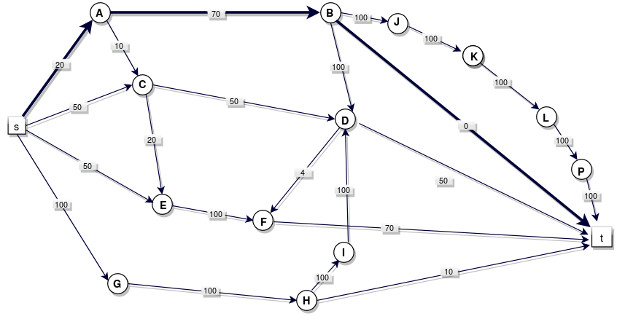
\includegraphics{definitions/EK2.jpg}
        \end{adjustbox}
    
\end{center}

Las etiquetas en los vértices muestran la capacidad remanente. La tabla de capacidades actualzada queda así:

 

\begin{center}
$\begin{array}{llllll} \overrightarrow{sA}: \cancel{100}20& \overrightarrow{AB}: \cancel{150} 70&\overrightarrow{BJ}: 100&\overrightarrow{DF}: 4&\overrightarrow{Ht}: 10&\overrightarrow{KL}: 100\\ \overrightarrow{sC}: 50& \overrightarrow{AC}: 10&\overrightarrow{CD}: 50&\overrightarrow{EF}: 100&\overrightarrow{HI}: 100&\overrightarrow{LP}: 100\\ \overrightarrow{sE}: 50& \overrightarrow{Bt}: \cancel{80} 0&\overrightarrow{CE}: 20&\overrightarrow{Ft}: 70&\overrightarrow{ID}: 100&\overrightarrow{Pt}: 100\\ \overrightarrow{sG}: 100& \overrightarrow{BD}: 100&\overrightarrow{Dt}: 50&\overrightarrow{GH}: 100&\overrightarrow{JK}: 100&\\ \end{array}$
\end{center}

Es a partir de esta representación en forma de tabla que podemos deducir los valores que toma $f_1$ (el flujo correspondiente al paso 1):

\begin{center}
$f_1(\overrightarrow{xy}) = \begin{cases} 80 & \text{ en los lados } \overrightarrow{sA}, \overrightarrow{AB},\overrightarrow{Bt}\\ 0 & \text{ en los otros lados} \end{cases} $
\end{center}

\subsubsection*{Paso 2}

A partir de este paso, los cómputos se abrevian y se muestra la cola BFS, y el camino aumentante y $\varepsilon$ así como la tabla actualizada.

\textbf{Cola}

$\begin{array}{ccccccccccc} \cancel{s} & \cancel{A} & \cancel{C} & \cancel{E} & \cancel{G} & \cancel{B} & D& F& H &J &t\\ & s & s & s & s & A & C & E&G&B &D\\ & 20 & 50 & 50 & 100 & 20 & 50 &50 & 100 & 20 &50 \end{array}$

\textbf{Camino aumentante}

$sCDt:50$

\textbf{Capacidades}

$\begin{array}{llllll} \overrightarrow{sA}: \cancel{100}20& \overrightarrow{AB}: \cancel{150} 70&\overrightarrow{BJ}: 100&\overrightarrow{DF}: 4&\overrightarrow{Ht}: 10&\overrightarrow{KL}: 100\\ \overrightarrow{sC}: \cancel{50}0& \overrightarrow{AC}: 10&\overrightarrow{CD}: \cancel{50}0&\overrightarrow{EF}: 100&\overrightarrow{HI}: 100&\overrightarrow{LP}: 100\\ \overrightarrow{sE}: 50& \overrightarrow{Bt}: \cancel{80} 0&\overrightarrow{CE}: 20&\overrightarrow{Ft}: 70&\overrightarrow{ID}: 100&\overrightarrow{Pt}: 100\\ \overrightarrow{sG}: 100& \overrightarrow{BD}: 100&\overrightarrow{Dt}: \cancel{50}0&\overrightarrow{GH}: 100&\overrightarrow{JK}: 100&\\ \end{array}$

\subsubsection*{Paso 3}

\textbf{Cola}

\textbf{$\begin{array}{ccccccccccc} \cancel{s} & \cancel{A} & \cancel{E} & \cancel{G} & \cancel{B} & \cancel{C} & F & H & D &J& t\\ & s & s & s & A & A & E &G & B & B & F\\ & 20 & 50 & 100 & 20 & 10 & 50& 100 & 20 & 20 & 50 \end{array}$}

\textbf{Camino Aumentante}

\textbf{$sEFt:50$}

\textbf{Capacidades}

$\begin{array}{llllll} \overrightarrow{sA}: \cancel{100}20& \overrightarrow{AB}: \cancel{150} 70&\overrightarrow{BJ}: 100&\overrightarrow{DF}: 4&\overrightarrow{Ht}: 10&\overrightarrow{KL}: 100\\ \overrightarrow{sC}: \cancel{50}& \overrightarrow{AC}: 10&\overrightarrow{CD}: \cancel{50}&\overrightarrow{EF}: \cancel{100}50&\overrightarrow{HI}: 100&\overrightarrow{LP}: 100\\ \overrightarrow{sE}: \cancel{50}& \overrightarrow{Bt}: \cancel{80}&\overrightarrow{CE}: 20&\overrightarrow{Ft}: \cancel{70}20&\overrightarrow{ID}: 100&\overrightarrow{Pt}: 100\\ \overrightarrow{sG}: 100& \overrightarrow{BD}: 100&\overrightarrow{Dt}: \cancel{50}&\overrightarrow{GH}: 100&\overrightarrow{JK}: 100&\\ \end{array}$

\subsubsection*{Paso 4}

\textbf{Cola}

$\begin{array}{cccccccccc} \cancel{s} & \cancel{A} & \cancel{G} & \cancel{B} & \cancel{C} & H &D &J & E & t\\ & s & s & A & A &G & B &B & C &H\\ & 20 & 100 & 20 & 10 &100 &20 &20 & 10 & 10 \end{array}$

\textbf{Camino aumentante}

\textbf{$sGHt:10$}

\textbf{Capacidades}

$\begin{array}{llllll} \overrightarrow{sA}: \cancel{100}20& \overrightarrow{AB}: \cancel{150} 70&\overrightarrow{BJ}: 100&\overrightarrow{DF}: 4&\overrightarrow{Ht}: \cancel{10}&\overrightarrow{KL}: 100\\ \overrightarrow{sC}: \cancel{50}& \overrightarrow{AC}: 10&\overrightarrow{CD}: \cancel{50}&\overrightarrow{EF}: \cancel{100}50&\overrightarrow{HI}: 100&\overrightarrow{LP}: 100\\ \overrightarrow{sE}: \cancel{50}& \overrightarrow{Bt}: \cancel{80}&\overrightarrow{CE}: 20&\overrightarrow{Ft}: \cancel{70}20&\overrightarrow{ID}: 100&\overrightarrow{Pt}: 100\\ \overrightarrow{sG}: \cancel{100}90& \overrightarrow{BD}: 100&\overrightarrow{Dt}: \cancel{50}&\overrightarrow{GH}: \cancel{100}90&\overrightarrow{JK}: 100&\\ \end{array}$

\subsubsection*{Paso 5}

\textbf{Cola}

$\begin{array}{ccccccccccccc} \cancel{s} & \cancel{A} & \cancel{G} &\cancel{B} & \cancel{C} & \cancel{H} & \cancel{D} & \cancel{J} &\cancel{E} & \cancel{I} & F & K & t\\ & s & s & A &A & G & B &B & C &H & D &J &F\\ & 20 & 90 & 20 & 10&90 &20 &20 &10 & 90 & 4 & 20 & 4 \end{array}$

\textbf{Camino aumentante}

$sABDFt:4$

\textbf{Capacidades}

$\begin{array}{llllll} \overrightarrow{sA}: \cancel{100}\cancel{20}16& \overrightarrow{AB}: \cancel{150} \cancel{70}66&\overrightarrow{BJ}: 100&\overrightarrow{DF}: \cancel{4}&\overrightarrow{Ht}: \cancel{10}&\overrightarrow{KL}: 100\\ \overrightarrow{sC}: \cancel{50}& \overrightarrow{AC}: 10&\overrightarrow{CD}: \cancel{50}&\overrightarrow{EF}: \cancel{100}50&\overrightarrow{HI}: 100&\overrightarrow{LP}: 100\\ \overrightarrow{sE}: \cancel{50}& \overrightarrow{Bt}: \cancel{80}&\overrightarrow{CE}: 20&\overrightarrow{Ft}: \cancel{70}\cancel{20}16&\overrightarrow{ID}: 100&\overrightarrow{Pt}: 100\\ \overrightarrow{sG}: \cancel{100}90& \overrightarrow{BD}: \cancel{100}96&\overrightarrow{Dt}: \cancel{50}&\overrightarrow{GH}: \cancel{100}90&\overrightarrow{JK}: 100&\\ \end{array}$

\subsubsection*{Paso 6}

\textbf{Cola}

$\begin{array}{cccccccccccccc} \cancel{s} & \cancel{A} & \cancel{G} & \cancel{B} & \cancel{C} & \cancel{H} & \cancel{D} & \cancel{J} & \cancel{E} & \cancel{I} & \cancel{K} & F& t\\ & s & s & A & A & G & B &B & C & H & J & E &F\\ & 16 & 90 & 16 & 10 & 90&16& 16 & 10 & 90 & 16 & 10 &10 \end{array}$

\textbf{Camino aumentante}

$sACEFt:10$

\textbf{Capacidades}

$\begin{array}{llllll} \overrightarrow{sA}: \cancel{100}\cancel{20}\cancel{16}6& \overrightarrow{AB}: \cancel{150} \cancel{70}66&\overrightarrow{BJ}: 100&\overrightarrow{DF}: \cancel{4}&\overrightarrow{Ht}: \cancel{10}&\overrightarrow{KL}: 100\\ \overrightarrow{sC}: \cancel{50}& \overrightarrow{AC}: \cancel{10}&\overrightarrow{CD}: \cancel{50}&\overrightarrow{EF}: \cancel{100}\cancel{50}40&\overrightarrow{HI}: 100&\overrightarrow{LP}: 100\\ \overrightarrow{sE}: \cancel{50}& \overrightarrow{Bt}: \cancel{80}&\overrightarrow{CE}: \cancel{20}10 &\overrightarrow{Ft}: \cancel{70}\cancel{20}\cancel{16}6&\overrightarrow{ID}: 100&\overrightarrow{Pt}: 100\\ \overrightarrow{sG}: \cancel{100}90& \overrightarrow{BD}: \cancel{100}96&\overrightarrow{Dt}: \cancel{50}&\overrightarrow{GH}: \cancel{100}90&\overrightarrow{JK}: 100&\\ \end{array}$

\subsubsection*{Paso 7}

\textbf{Cola}

$\begin{array}{ccccccccccccccc} \cancel{s} & \cancel{A} & \cancel{G} &\cancel{B} & \cancel{H} & \cancel{D} & \cancel{J} & \cancel{I} & \cancel{C} & \cancel{K} & \cancel{E} & \cancel{L}& F & P & t\\ & s & s & A & G & B &B & H & D^{-} & J & C & K & E & L & F\\ & 6 & 90 & 6 & 90 &6 & 6 & 90 & 6 &6 & 6 & 6 & 6 & 6 & 6 \end{array}$

Hemos incluido el símbolo $D^-$ para recordar el hecho de que en realidad $D$ está devolviendo flujo a $C$. Recordemos que en el network existe el lado $\overrightarrow{CD}$, por lo que la sucesión $\overleftarrow{DC}$ es en realidad un lado backwards.

\textbf{Camino aumentante}

\textbf{$sAB\overleftarrow{DC}EFt:6$}

\textbf{Capacidades}

$\begin{array}{llllll} \overrightarrow{sA}: \cancel{100}\cancel{20}\cancel{16}\cancel{6}& \overrightarrow{AB}: \cancel{150} \cancel{70}\cancel{66}60&\overrightarrow{BJ}: 100&\overrightarrow{DF}: \cancel{4}&\overrightarrow{Ht}: \cancel{10}&\overrightarrow{KL}: 100\\ \overrightarrow{sC}: \cancel{50}& \overrightarrow{AC}: \cancel{10}&\overrightarrow{CD}: \cancel{50}6&\overrightarrow{EF}: \cancel{100}\cancel{50}\cancel{40}34&\overrightarrow{HI}: 100&\overrightarrow{LP}: 100\\ \overrightarrow{sE}: \cancel{50}& \overrightarrow{Bt}: \cancel{80}&\overrightarrow{CE}: \cancel{20}\cancel{10}4 &\overrightarrow{Ft}: \cancel{70}\cancel{20}\cancel{16}\cancel{6}&\overrightarrow{ID}: 100&\overrightarrow{Pt}: 100\\ \overrightarrow{sG}: \cancel{100}90& \overrightarrow{BD}: \cancel{100}\cancel{96}90&\overrightarrow{Dt}: \cancel{50}&\overrightarrow{GH}: \cancel{100}90&\overrightarrow{JK}: 100&\\ \end{array}$

\subsubsection*{Paso 8}

\textbf{Cola}

$\begin{array}{ccccccccccccccc} \cancel{s} & \cancel{G} & \cancel{H} & \cancel{I} & \cancel{D} & \cancel{B} &\cancel{C} & \cancel{F} &\cancel{A} & \cancel{J} &\cancel{E} & \cancel{K}& \cancel{L} &P & t\\ &s & G &H & I & D^- &D^- & D^- & B^- &B & F^-&J & K & L& P\\ & 90 & 90& 90 & 90 & 10 & 44 & 4&10 &10 & 4 & 10 & 10 & 10 & 10 \end{array}$

\textbf{Camino aumentante}

\textbf{$sGHI\overleftarrow{DB}JKLPt:10$}

\textbf{Capacidades}

$\begin{array}{llllll} \overrightarrow{sA}: \cancel{100}\cancel{20}\cancel{16}\cancel{6}& \overrightarrow{AB}: \cancel{150} \cancel{70}\cancel{66}60&\overrightarrow{BJ}: \cancel{100}90& \overrightarrow{DF}: \cancel{4}&\overrightarrow{Ht}: \cancel{10}&\overrightarrow{KL}: \cancel{100}90\\ \overrightarrow{sC}: \cancel{50}& \overrightarrow{AC}: \cancel{10}&\overrightarrow{CD}: \cancel{50}6&\overrightarrow{EF}: \cancel{100}\cancel{50}\cancel{40}34&\overrightarrow{HI}: \cancel{100}90&\overrightarrow{LP}: \cancel{100}90\\ \overrightarrow{sE}: \cancel{50}& \overrightarrow{Bt}: \cancel{80}&\overrightarrow{CE}: \cancel{20}\cancel{10}4 &\overrightarrow{Ft}: \cancel{70}\cancel{20}\cancel{16}\cancel{6}&\overrightarrow{ID}: \cancel{100}90&\overrightarrow{Pt}: \cancel{100}\cancel{90}80\\ \overrightarrow{sG}: \cancel{100}\cancel{90}80& \overrightarrow{BD}: \cancel{100}\cancel{96}\cancel{90}100&\overrightarrow{Dt}: \cancel{50}&\overrightarrow{GH}: \cancel{100}\cancel{90}80&\overrightarrow{JK}: \cancel{100}90&\\ \end{array}$

\subsubsection*{Paso 9}

\textbf{Cola}

\textbf{$\begin{array}{ccccccccccccccc} \cancel{s} & \cancel{G} & \cancel{H} & \cancel{I} & \cancel{D}& \cancel{C } &\cancel{F} & \cancel{A} & \cancel{E} & \cancel{B} & \cancel{J} & \cancel{K} & \cancel{L} &P & t\\ & s & G & H & I & D^- &D^-& C^- & C &A & B &J &K &L &P\\ & 80 & 80 & 80 & 80 & 44& 4 & 10 & 4 & 10 & 10& 10 & 10 & 10 & 10 \end{array}$}

\textbf{Camino aumentante}

\textbf{$sGHI\overleftarrow{D}\overleftarrow{CA}BJKLPt:10$}

\textbf{Capacidades}

$\begin{array}{llllll} \overrightarrow{sA}: \cancel{100}\cancel{20}\cancel{16}\cancel{6}& \overrightarrow{AB}: \cancel{150} \cancel{70}\cancel{66}\cancel{60}50&\overrightarrow{BJ}: \cancel{100}90& \overrightarrow{DF}: \cancel{4}&\overrightarrow{Ht}: \cancel{10}&\overrightarrow{KL}: \cancel{100}\cancel{90}80\\ \overrightarrow{sC}: \cancel{50}& \overrightarrow{AC}: \cancel{10}\cancel{0}10&\overrightarrow{CD}: \cancel{50}\cancel{6}16&\overrightarrow{EF}: \cancel{100}\cancel{50}\cancel{40}34&\overrightarrow{HI}: \cancel{100}\cancel{90}80&\overrightarrow{LP}: \cancel{100}\cancel{90}80\\ \overrightarrow{sE}: \cancel{50}& \overrightarrow{Bt}: \cancel{80}&\overrightarrow{CE}: \cancel{20}\cancel{10}4 &\overrightarrow{Ft}: \cancel{70}\cancel{20}\cancel{16}\cancel{6}&\overrightarrow{ID}: \cancel{100}\cancel{90}80&\overrightarrow{Pt}: \cancel{100}90\\ \overrightarrow{sG}: \cancel{100}\cancel{90}\cancel{80}70& \overrightarrow{BD}: \cancel{100}\cancel{96}\cancel{90}100&\overrightarrow{Dt}: \cancel{50}&\overrightarrow{GH}: \cancel{100}\cancel{90}\cancel{80}70&\overrightarrow{JK}: \cancel{100}\cancel{90}80&\\ \end{array}$

\subsubsection*{Paso 10}

\textbf{Cola}

\textbf{$\begin{array}{cccccccc} \cancel{s} & \cancel{G} & \cancel{H} & \cancel{I} & \cancel{D} & \cancel{C} & \cancel{F} & \cancel{E}\\ & s & G & H & I & D^- & D^- & C^- \\ & 70 & 70 & 70 & 70 & 34 & 4 & 4 \end{array}$}

La cola se vació y nunca llegamos a $t$. Esto significa que hemos llegado al final del algoritmo, porque ya no se puede construir un camino aumentante entre $s$ y $t$.

 

Valor del flujo $v(f_{MAX}) = f_{MAX} (\overrightarrow{sA}) + f_{MAX} (\overrightarrow{sC}) + f_{MAX} (\overrightarrow{sE}) + f_{MAX} (\overrightarrow{sG}) = 230$.

Además (y como comprobación de que obtuvimos un resultado correcto) la cola final (la que no completa un camino aumentante) es un corte minimal y su capacidad debe ser igual al valor del flujo maximal obtenido:


$S= \{s, G, H, I, D, C, E, F\}$

$CAP(S) = C(S, V- S) = c(\overrightarrow{sA}) + c(\overrightarrow{Ht}) + c(\overrightarrow{Dt}) + c(\overrightarrow{Ft}) = 100 + 10 + 50 + 70 = 230$

\section*{Complejidad y correctitud de Edmonds-Karp}

La complejidad de Edmonds-Karp es $O(nm^2)$. En particular, siempre termina.

Observación: Para grafos ralos (es decir, con pocos lados) $m$ se acerca a $n$ y podemos decir que la complejidad de Edmonds-Karp es $O(n^3)$, mientras que en grafos no ralos (cercanos a grafos completos), $m$ se aproxima a $n^2$ y podemos decir que la complejidad de Edmonds-Karp es $O(n^5)$.

\subsubsection*{Prueba}

Probaremos primero un hecho por inducción. Para enunciarlo, sea $f_0 = 0, f_1, f_2, f_3, \dots$ la sucesión de flujos producida por el algoritmo Edmonds-Karp. Hasta ahora no sabemos si esa sucesión termina, así que puede ser una sucesión infinita.

Para cada paso $k$ del algoritmo y cada vértice $x$ perteneciente al network, definimos dos funciones:

\begin{itemize}

	\item $d_k(s) = 0$
	\item $d_k(x) = $ longitud (número de lados) del camino aumentante más corto entre $s$ y $x$, si tal camino existe
\end{itemize}

y

\begin{itemize}

	\item $b_k(t) = 0$
	\item $b_k(x) = $ longitud del camino aumentante más corto entre $x$ y $t$, si tal camino existe.
\end{itemize}

Queremos probar que

\begin{center}
$d_k(x) \leq d_{k+1}(x)$ y $b_k(x) \leq b_{k+1}(x)$
\end{center}

En la práctica, al correr el algoritmo, esto se traduce en que los caminos aumentantes encontrados nunca son más cortos que el anterior. Queremos probar que esto se cumple siempre. Lo probaremos para $d_k$, siendo la prueba para $b_k$ análoga.

\subsubsection*{Hipótesis inductiva (inducción en $i$)}

$H(i)$: Para todo vértice $z$ tal que $d_{k+1}(z) \leq i$ vale que $d_k(z) \leq d_{k+1}(z)$

Esta es la propiedad que queremos probar que se cumple para todo número natural $i$. Dicho en palabras, si la longitud del camino aumentante más corto entre $s$ y $z$ en el paso $k+1$ (con respecto al flujo $f_k$) es menor o igual que $i$, entonces dicha longitud es mayor o igual a la longitud del camino aumentante más corto entre $s$ y $z$ con respecto al paso anterior (paso $k$, relativo al flujo $f_{k-1}$).

\subsubsection*{Caso base: $H(0)$.}

Tenemos que ver que para todo vértice $z$ tal que $d_{k+1}(z) \leq 0$ vale que $d_k(z) \leq d_{k+1}(z)$. Pero si $d_{k+1}(z) \leq 0$ debe ser $z=s$, entonces $d_k(z) = d_k(s) = 0 \leq d_{k+1}(s) = d_{k+1}(z)$. La siguiente imagen ayuda a comprender esta situación: $d_j(s) = 0 $ para todo $j \in \mathbb{N}_0$.

\begin{center}

    \begin{adjustbox}{max size={\textwidth}{\textheight}}
        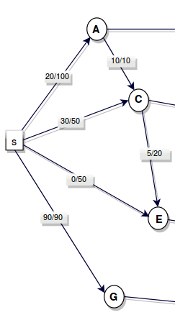
\includegraphics{definitions/prueba_EK1.jpg}
        \end{adjustbox}
    
\end{center}

 

\subsubsection*{Caso inductivo: $H(i) \Rightarrow H(i+1)$}

Sea $z$ con $d_{k+1} \leq i + 1$. Hay dos posibilidades, o bien $d_{k+1}\leq i$ o bien $d_{k+1}(z) = i + 1$. En el primer caso, por hipótesis inductiva sabemos que $d_k(z) \leq d_{k+1}(z)$. Concentrémonos entonces en este último caso.

Si $d_{k+1}(z) = i + 1$ entonces existe un camino aumentante (relativo a $f_k$) de la forma

\begin{center}
$z_0 = s, z_1, z_2, \dots, z_i, z_{i+1}=z$
\end{center}

\begin{center}

    \begin{adjustbox}{max size={\textwidth}{\textheight}}
        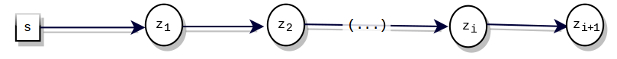
\includegraphics{definitions/prueba_EK2.jpg}
        \end{adjustbox}
    
\end{center}

Sea $x = z_i$ (el vértice anterior en dicho camino aumentante).

\textbf{CASO 1.} Existe algún camino aumentante relativo a $f_{k-1}$ de la forma 

\begin{center}
$z_0=s, z_1,\dots,x,z$
\end{center}

\begin{center}

    \begin{adjustbox}{max size={\textwidth}{\textheight}}
        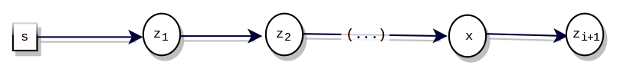
\includegraphics{definitions/prueba_EK3.jpg}
        \end{adjustbox}
    
\end{center}

Notar que la situación en el paso anterior no necesariamente era igual, ya que no sabemos qué pasa entre $z_2$ y $z_i = x$ en ninguno de los dos paso (tanto en el paso $k$ como en el paso $k+1$). Sin embargo, podemos afirmar que $d_k(z) \leq d_k(x)+1$, pues al haber un camino $s, \dots,x,z $ de longitud $d_k(x)+1$ sabemos que el mínimo de las longitudes de los caminos aumentantes entre $s$ y $z$ debe ser menor o igual a eso (puede haber otros menores). La utilidad de este hecho se verá al concluir el caso 2.

\textbf{CASO 2.} No existe un tal camino relativo a $f_{k-1}$.Pero recordemos que estamos considerando que $d_{k+1}(z)=i+1$, o sea que por definición sí existe relativo a $f_k$(ej: $z_0=s,z_1,\dots,z_i,z_{i+1} = z$). El "pseudolado" $xz$ no está disponible en el paso $k$: o bien $\exists\;\overrightarrow{xz}$ y está saturado, o bien $\exists\;\overrightarrow{zx}$ y está vacío. Pero el paso $k$ se hace relativo al $f_{k-1}$, y cuando llegamos la paso $k+1$ el lado $xz$ está disponible de una de dos maneras:

\begin{enumerate}

	\item $f_{k-1}(\overrightarrow{xz}) =c(\overrightarrow{xz})$ pero $f_k(\overrightarrow{xz}) < c (\overrightarrow{xz})$, o bien
	\item $f_{k+1}(\overrightarrow{zx}) = 0$ pero $f_k(\overrightarrow{zx}) > 0$
\end{enumerate}

1 $\Rightarrow$ $f_k$ devuelve flujo por $\overrightarrow{xz}$, por lo tanto para construir $f_k$ utilizamos $\overrightarrow{zx}$ (lado backwards), usando un camino

\begin{center}
$z_0=s, z_1, \dots, z,x$
\end{center}

\begin{center}

    \begin{adjustbox}{max size={\textwidth}{\textheight}}
        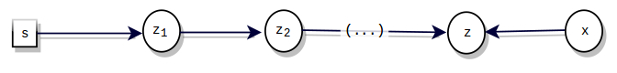
\includegraphics{definitions/prueba_EK4.jpg}
        \end{adjustbox}
    
\end{center}

2 $\Rightarrow$ $f_k$ manda flujo por $\overrightarrow{zx}$ y se concluye lo mismo que antes: tiene  que haber un camino (y lo usamos) de la forma

\begin{center}
$z_0=s, z_1, \dots, z,x$
\end{center}

\begin{center}

    \begin{adjustbox}{max size={\textwidth}{\textheight}}
        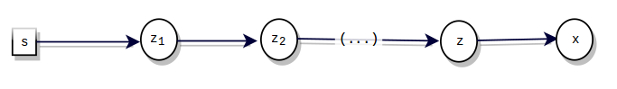
\includegraphics{definitions/prueba_EK5.jpg}
        \end{adjustbox}
    
\end{center}

Como Edmonds-Karp funciona con BFS, este camino usado para construir $f_k$ es de longitud mínima, por ende

\begin{center}
$d_k(x) = d_k(z)+1$
\end{center}

Esto implica que $d_k(z) = d_k(x)-1\leq d_k(x) + 1$.

Notemos que tanto en el \textbf{CASO 1} como en el \textbf{CASO 2} llegamos a la conclusión de que

\begin{center}
$d_k(z) \leq d_k(x)+1 \quad \quad(1)$
\end{center}

Ahora bien, $d_{k+1}(x) = d_{k+1}(z_i) = i$, por lo tanto vale la hipótesis inductiva para $x$ y entonces tenemos que

\begin{center}
$d_k(x) \leq d_{k+1}(x)\quad\quad (2)$
\end{center}

Por $(1)$ y $(2)$ se concluye que $d_k(z) \leq d_k(x) + 1\leq d_{k+1}(x) +1 = i + 1 = d_{k+1}(z)$.

Así concluye la prueba de que la propiedad $H(i)$ vale para todo $i\in \mathbb{N}_0$.

Con esta herramienta, analicemos la complejidad del algoritmo.

\vspace{0.5cm}\hrule\vspace{0.5cm}
 

El \textbf{while} interno (\textbf{while} $Q \neq \emptyset$) implementa

\begin{itemize}

	\item BFS, $O(\sum\limits_{x\in V} d(x)) = O(2m) = O(m)$
	\item Aumentar el flujo, $O(n)$, pues aumenta el flujo a lo largo de un camino aumentante, que tiene a lo sumo $n$ vértices.
\end{itemize}

Luego, el \textbf{while} interno tiene complejidad $O(m) + O(n) = O(m)$

Por lo tanto, la complejidad de Edmonds-Karp es:

\begin{center}
$O(m) * $ (número de veces que se ejecuta el \textbf{while} interno)
\end{center}

Es decir, $O(m)$ por un número determinado de veces, hasta que deja de ser cierta la condición $\text{done} \Leftrightarrow t\not \in S$. Es decir, hasta que no podamos encontrar un camino aumentante entre $s$ y $t$.

Pero el número de caminos aumentantes que podemos encontrar es menor o igual al número de lados $(m)$ por la cantidad de veces que un lado se puede saturar o llenar. Necesitamos acotar este último valor.

Supongamos que al construir el flujo en el paso $k$, el lado $\overrightarrow{xz}$ se satura o el lado $\overrightarrow{zx}$ se vacía, tenemos camino

\begin{center}
$s\dots xz\dots t$
\end{center}

y este camino se utiliza para construir $f_k$. Tenemos que

\begin{center}
\begin{align*} d_k(t) &= d_k(x) + b_k(x)\\ &= d_k(x)+1+b_k(z) \end{align*}
\end{center}

Como $\overrightarrow{xz}$ se saturó o $\overrightarrow{zx}$ se vació, para volverlo a saturar (vaciar) lo tengo que vaciar (llenar al menos un poco). Por lo tanto, antes de saturarlo o vaciarlo dbe haber un $j$ tal que para construir $f_j$ debemos usar un camino aumentante de la forma

\begin{center}
$s\dots zx\dots t$
\end{center}

Por lo tanto,

\begin{center}
\begin{align*} d_j(t) &= d_j(x) + b_j(x)\\ &= d_j(z)+1+b_j(x)\\ &\geq d_k(z) + 1 + b_k(z)\\ &= (d_k(x)+1) + 1 + b_k(x)\\ &= d_k(t) + 2 \end{align*}
\end{center}

Por lo tanto, antes de poder saturarse o vaciarse otra vez, la longitud del menor camino aumentante de $s$ a $t$ debe aumentar en al menos $2$. Concluimos que puede haber a lo sumo $n/2$ caminos aumentantes.

Entonces, la complejidad de Edmonds-Karp es:

\begin{center}
$O(m.m.n)=O(nm^2)$
\end{center}

\section*{Dinic}

Se trata de un algoritmo para buscar el flujo maximal en un network, que constituye una mejora en la complejidad del algoritmo de Edmonds-Karp.

\subsubsection*{Idea general}

Dado un network $N$ y un flujo $f$, se construye un network auxiliar $NA_f$, donde se encuentra un flujo bloqueante $g$. Con $f$ y $g$ se construye $f^*$.

\subsubsection*{Network Residual}

El Network Auxilar de Dinic constituye un refinamiento del Network Residual ($NR$). En un $NR$, están todos los vértices, y por cada lado $\overrightarrow{xy} \in E(N)$ se crean $0$, $1$ o $2$ lados:

\begin{itemize}

	\item Si  $f(\overrightarrow{xy}) < c(\overrightarrow{xy}) $ en $N$, se crea el lado $\overrightarrow{xy}$ en $NR$, con capacidad $c(\overrightarrow{xy}) - f(\overrightarrow{xy})$ (capacidad \textbf{residual}).
	\item Si $f(\overrightarrow{xy}) > 0$ en $N$, se crea el lado $\overrightarrow{yx}$ en $NR$, con capacidad $f(\overrightarrow{xy})$.
\end{itemize}

\begin{center}

    \begin{adjustbox}{max size={\textwidth}{\textheight}}
        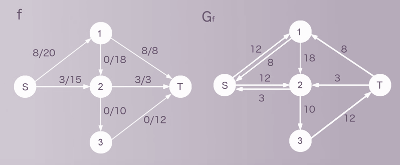
\includegraphics{definitions/NR.png}
        \end{adjustbox}
    
\end{center}

\subsubsection*{Network Auxiliar}

El Network Auxiliar ($NA$) es un subnetwork del Network Residual, obtenido de la siguiente forma:

\begin{enumerate}

	\item Se calculan las distancias de $s$ a $x$ para todo vértice $x$ como en la prueba de Edmonds-Karp (longitud del menor camino aumentante entre $s$ y $x$).
	\item Sólo dejamos el lado $\overrightarrow{xy}$ si $d(y) = d(x) + 1$
	\item Eliminamos todos los vértices $x$ y los lados incidentes con ellos tales que $d(x) \geq d(t)$, a excepción del mismo $t$.
\end{enumerate}

Por construcción, el Network auxiliar será un network por niveles:

\begin{center}

    \begin{adjustbox}{max size={\textwidth}{\textheight}}
        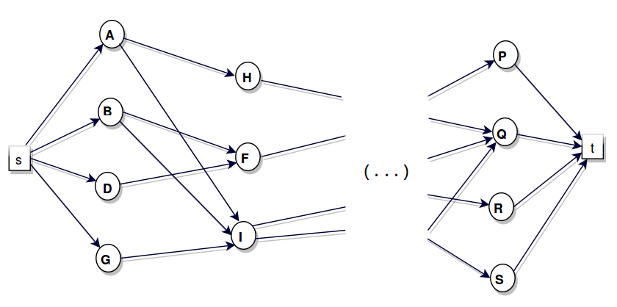
\includegraphics{definitions/dinic_1.jpg}
        \end{adjustbox}
    
\end{center}

Trabajar en este network es más fácil utilizando DFS.

\subsubsection*{Blocking Flow}

Un Blocking Flow o flujo bloqueante en un $NA$ es un flujo $g$ tal que todo camino dirigido (no aumentante) de $s$ a $t$ tiene un lado $\overrightarrow{xy}$ con $g(\overrightarrow{xy}) = c(\overrightarrow{xy})$. Todos los caminos tienen al menos un lado saturado y por lo tanto ya no se puede mandar más por ningún lado.

\subsubsection*{Algoritmo}

\begin{enumerate}

	\item Construir un $NA$ utilizando BFS.
	\item Encontrar flujo bloqueante usando greedy con DFS.
	\item Repetir hasta que no se pueda construir un $NA$ porque $s$ y $t$ quedan inconcexos.
\end{enumerate}

Si $f$ es el flujo actual en el network $N$, $g$ es el flujo bloqueante obtenido sobre $NA$, entonces el flujo $f^*$ se construye así:

\begin{itemize}

	\item Si $\overrightarrow{xy}\in E(NA)$ viene de $\overrightarrow{xy} \in E(N)$, entonces $f^*(\overrightarrow{xy}) = f(\overrightarrow{xy}) + g(\overrightarrow{xy})$ donde $f$ es el flujo del paso anterior en el network $N$ y $g$ es el flujo en el $NA$.
	\item Si $\overrightarrow{xy} \in E(NA)$ corresponde a $\overrightarrow{yx} \in E(N)$, entonces $f^*(\overrightarrow{yx}) = f(\overrightarrow{yx}) - g(\overrightarrow{xy})$
\end{itemize}

\subsubsection*{Pseudocódigo}


    \lstset{
        commentstyle=\color{mygreen},
        keywordstyle=\color{myred},
        frame=single,
        backgroundcolor=\color{gray!10},
        inputencoding=utf8,
        extendedchars=true,
        mathescape=true,
        breaklines=true,
        literate={á}{{\'a}}1 {é}{{\'e}}1 {í}{{\'i}}1 {ó}{{\'o}}1 {ú}{{\'u}}1 {ñ}{{\~n}}1
    }
    \begin{lstlisting}[language=pseudo]
procedure DINIC(Input: NA, Output: g bloqueante en NA)
// a partir de aquí, todos los símbolos hacen referencia al network auxiliar
g = 0
d = $d(t)$
P = array con [0, 1, ..., $d(t)$] elementos
done = False
while not done:
    i = 0
    while (i $<$ d) and not done:
        // buscamos llegar hasta $t$

        if ($\Gamma^+($P[i]$) \neq \emptyset$):
            // AVANZAR
            P[i+1] = algún vértice en $\Gamma^+($P[i]$)$
            i++;
            // FIN AVANZAR
        else:
            if i $\neq$ 0:
                // borramos el lado para no volver a intentarlo
                // RETROCEDER
                Borrar P[i-1]P[i] del NA
                i--;
                // FIN RETROCEDER
            else:
                 done = True 
    if i = d:
        // tenemos camino aumentante entre $s$ y $t$
        // INCREMENTAR
        $\varepsilon = \min\{c($P[i]P[i+1]$)-g($P[i]P[i+1]$) \;\forall \; 0 \leq i \leq d\}$
        for i= 0 to d -1:
            g+= $\varepsilon$
            if $g($P[i]P[i+1]$)$ = $c($P[i]P[i+1]$)$:
                borrar lado P[i]P[i+1] del NA
        // FIN INCREMENTAR
\end{lstlisting}

\section*{Max-Flow usando Dinic}

Calcularemos el flujo maximal del mismo network con el que se ejemplificó el algoritmo Edmonds-Karp:

\begin{center}

    \begin{adjustbox}{max size={\textwidth}{\textheight}}
        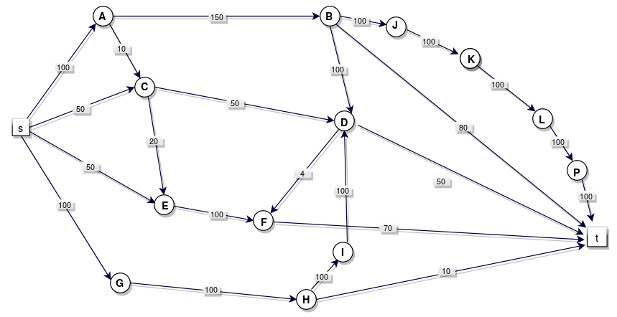
\includegraphics{definitions/EK1.jpg}
        \end{adjustbox}
    
\end{center}

dado por la siguiente lista de capacidades:

$\begin{array}{llllll} \overrightarrow{sA}: 100& \overrightarrow{AB}: 150&\overrightarrow{BJ}: 100&\overrightarrow{DF}: 4&\overrightarrow{Ht}:10&\overrightarrow{KL}: 100\\ \overrightarrow{sC}: 50& \overrightarrow{AC}: 10&\overrightarrow{CD}: 50&\overrightarrow{EF}: 100&\overrightarrow{HI}: 100&\overrightarrow{LP}: 100\\ \overrightarrow{sE}: 50& \overrightarrow{Bt}: 80&\overrightarrow{CE}: 20&\overrightarrow{Ft}: 70&\overrightarrow{ID}: 100&\overrightarrow{Pt}: 100\\ \overrightarrow{sG}:100& \overrightarrow{BD}: 100&\overrightarrow{Dt}:50&\overrightarrow{GH}: 100&\overrightarrow{JK}: 100&\\ \end{array}$

\subsubsection*{Paso 1}

El Network auxiliar es el siguiente:

\begin{center}

    \begin{adjustbox}{max size={\textwidth}{\textheight}}
        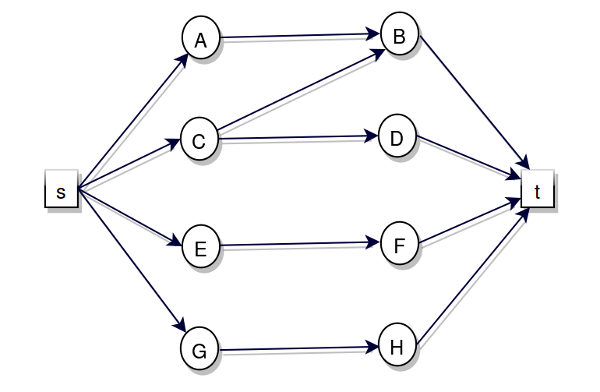
\includegraphics{definitions/D0.jpg}
        \end{adjustbox}
    
\end{center}

En la siguiente serie de imágenes se ve cómo se va fue construyendo dicho NA, utilizando BFS. Se empezó agregando a $s$:

\begin{center}


    \begin{adjustbox}{max size={\textwidth}{\textheight}}
        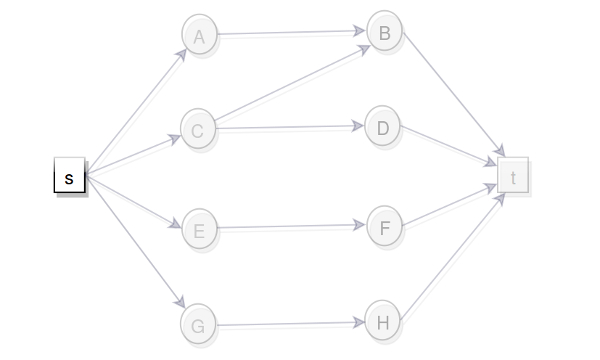
\includegraphics{definitions/D1.jpg}
        \end{adjustbox}
    
\end{center}

Como desde $s$ tenemos caminos aumentantes de longitud $1$ hasta $A$, $C$, $E$ y $G$, estos vértices son agregados por $s$ (y constituyen el primer nivel del NA).

\begin{center}

    \begin{adjustbox}{max size={\textwidth}{\textheight}}
        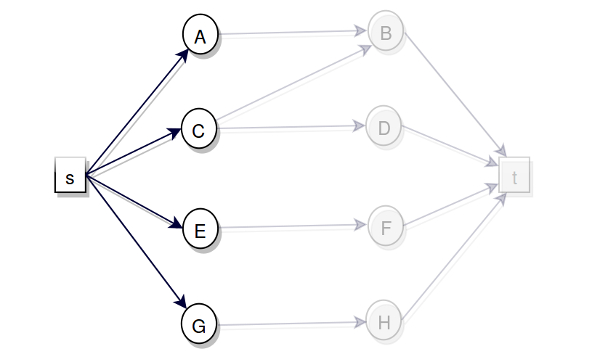
\includegraphics{definitions/D2.jpg}
        \end{adjustbox}
    
\end{center}

Corriendo BFS, terminamos de agregar a los vecinos de $s$ y continuamos con los vecinos de $A$. En el Network Residual, relativo al flujo $f_0 = 0$, los vecinos de $A$ para los cuales se cumple que la longitud del menor camino aumentante desde $s$ hasta ellos es $2$ ($1$ más que la longitud del menor camino aumentante hasta $A$, es decir $d(A) + 1$) son $\{B\}$, así que $A$ agrega a $B$ en el segundo nivel del NA (y lo encola para BFS).

Luego consideramos los vértices que podría agregar $C$. Estos son $\{B, D\}$. Notemos que aunque $B$ ya fue agregado por $A$, el lado $\overrightarrow{CB}$ cumple con las condiciones impuestas por el algoritmo: dejamos el lado $\overrightarrow{CB}$ porque este existe en el Network residual y además $d(B) = d(C) + 1$. Así agregamos los vecinos de $E$, de $F$, y se forma el segundo nivel del NA:

\begin{center}

    \begin{adjustbox}{max size={\textwidth}{\textheight}}
        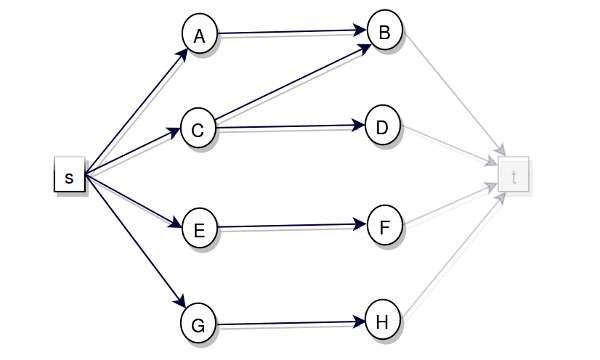
\includegraphics{definitions/D3.jpg}
        \end{adjustbox}
    
\end{center}

Como desde todos ellos se puede alcanzar $t$, el NA se concluye en el siguiente paso (por más que BFS podría seguir).

Ahora bien, utilizando DFS en el NA, buscamos caminos aumentantes. En cada camino aumentante, se satura o se vacía al menos un lado, de modo que el NA va "perdiendo alguno de sus lados".

\begin{center}

    \begin{adjustbox}{max size={\textwidth}{\textheight}}
        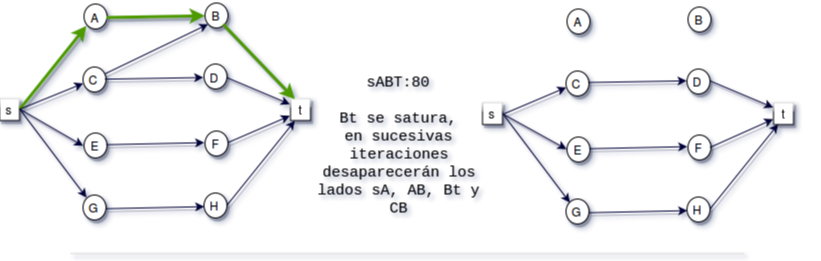
\includegraphics{definitions/dinic_ej_a.jpg}
        \end{adjustbox}
    
\end{center}

\begin{center}

    \begin{adjustbox}{max size={\textwidth}{\textheight}}
        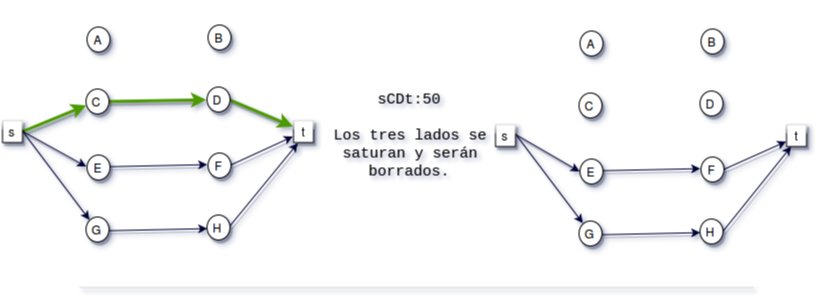
\includegraphics{definitions/dinic_ej_b.jpg}
        \end{adjustbox}
    
\end{center}

\begin{center}

    \begin{adjustbox}{max size={\textwidth}{\textheight}}
        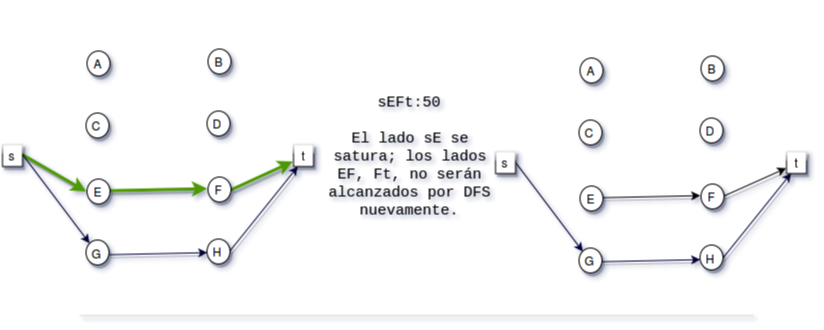
\includegraphics{definitions/dinic_ej_c.jpg}
        \end{adjustbox}
    
\end{center}

\begin{center}

    \begin{adjustbox}{max size={\textwidth}{\textheight}}
        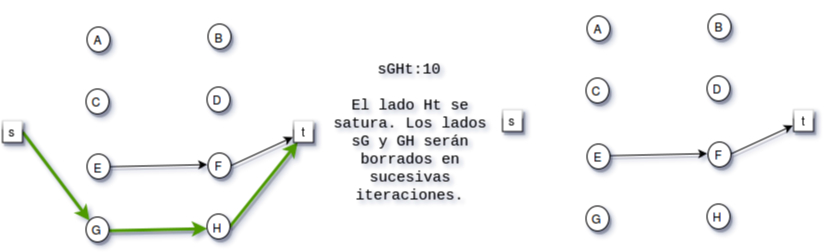
\includegraphics{definitions/dinic_ej_d.jpg}
        \end{adjustbox}
    
\end{center}

La lista de capacidades queda actualizada así:

$\begin{array}{llllll} \overrightarrow{sA}: \cancel{100}20& \overrightarrow{AB}: \cancel{150}70&\overrightarrow{BJ}: 100&\overrightarrow{DF}: 4&\overrightarrow{Ht}: \cancel{10}0&\overrightarrow{KL}: 100\\ \overrightarrow{sC}: \cancel{50}0& \overrightarrow{AC}: 10&\overrightarrow{CD}: \cancel{50}0&\overrightarrow{EF}: \cancel{100}50&\overrightarrow{HI}: 100&\overrightarrow{LP}: 100\\ \overrightarrow{sE}: \cancel{50}0& \overrightarrow{Bt}: \cancel{80}&\overrightarrow{CE}: 20&\overrightarrow{Ft}: \cancel{70}20&\overrightarrow{ID}: 100&\overrightarrow{Pt}: 100\\ \overrightarrow{sG}: \cancel{100}90& \overrightarrow{BD}: 100&\overrightarrow{Dt}: \cancel{50}0&\overrightarrow{GH}: \cancel{100}90&\overrightarrow{JK}: 100&\\ \end{array}$

\subsubsection*{Paso 2}

\textbf{Network Auxiliar:}

\begin{center}
\textbf{
    \begin{adjustbox}{max size={\textwidth}{\textheight}}
        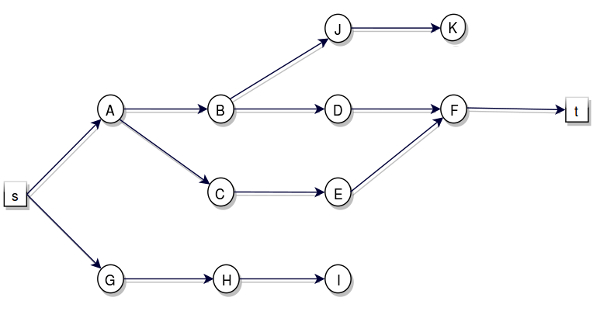
\includegraphics{definitions/D4.jpg}
        \end{adjustbox}
    }
\end{center}

\textbf{Caminos aumentantes}

\begin{align*} sABDFt&: 4\\ sACEFt&: 10 \end{align*}

\textbf{Capacidades actualizadas}

$\begin{array}{llllll} \overrightarrow{sA}: \cancel{100}\cancel{20}\cancel{16}6& \overrightarrow{AB}: \cancel{150}\cancel{70}66&\overrightarrow{BJ}: 100&\overrightarrow{DF}: \cancel{4} 0&\overrightarrow{Ht}: \cancel{10}0&\overrightarrow{KL}: 100\\ \overrightarrow{sC}: \cancel{50}0& \overrightarrow{AC}: \cancel{10}0&\overrightarrow{CD}: \cancel{50}0&\overrightarrow{EF}: \cancel{100}\cancel{50}40&\overrightarrow{HI}: 100&\overrightarrow{LP}: 100\\ \overrightarrow{sE}: \cancel{50}0& \overrightarrow{Bt}: \cancel{80}&\overrightarrow{CE}: \cancel{20}10&\overrightarrow{Ft}: \cancel{70}\cancel{20}\cancel{16}6 &\overrightarrow{ID}: 100&\overrightarrow{Pt}: 100\\ \overrightarrow{sG}: \cancel{100}90& \overrightarrow{BD}: \cancel{100}96&\overrightarrow{Dt}: \cancel{50}0&\overrightarrow{GH}: \cancel{100}90&\overrightarrow{JK}: 100&\\ \end{array}$

\subsubsection*{Paso 3}

\textbf{Network auxiliar}

\begin{center}
\textbf{
    \begin{adjustbox}{max size={\textwidth}{\textheight}}
        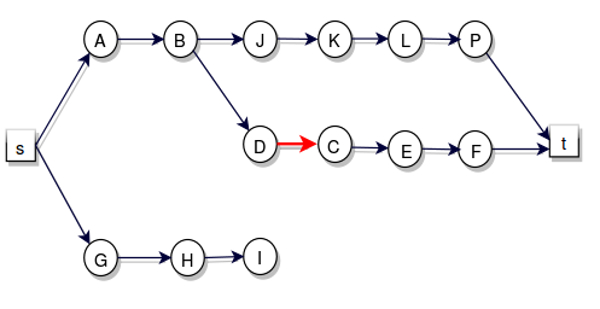
\includegraphics{definitions/D5.jpg}
        \end{adjustbox}
    }
\end{center}

Notar que el lado $\overrightarrow{DC}$ del network auxiliar corresponde a un lado backwards en el network original.

\textbf{Caminos aumentantes}

\textbf{\begin{align*} sAB\overleftarrow{DC}EFt &:6\\ \end{align*}}

\textbf{Capacidades actualizadas}

$\begin{array}{llllll} \overrightarrow{sA}: \cancel{100}\cancel{20}\cancel{16}\cancel{6}0& \overrightarrow{AB}: \cancel{150}\cancel{70}\cancel{66} 60&\overrightarrow{BJ}: 100&\overrightarrow{DF}: \cancel{4} 0&\overrightarrow{Ht}: \cancel{10}0&\overrightarrow{KL}: 100\\ \overrightarrow{sC}: \cancel{50}0& \overrightarrow{AC}: \cancel{10}0&\overrightarrow{CD}: \cancel{50}\cancel{0}6&\overrightarrow{EF}: \cancel{100}\cancel{50}\cancel{40}34&\overrightarrow{HI}: 100&\overrightarrow{LP}: 100\\ \overrightarrow{sE}: \cancel{50}0& \overrightarrow{Bt}: \cancel{80}&\overrightarrow{CE}: \cancel{20}\cancel{10}4&\overrightarrow{Ft}: \cancel{70}\cancel{20}\cancel{16}\cancel{6}0 &\overrightarrow{ID}: 100&\overrightarrow{Pt}: 100\\ \overrightarrow{sG}: \cancel{100}90& \overrightarrow{BD}: \cancel{100}\cancel{96}90&\overrightarrow{Dt}: \cancel{50}0&\overrightarrow{GH}: \cancel{100}90&\overrightarrow{JK}: 100&\\ \end{array}$

\subsubsection*{Paso 4}

\textbf{Network Auxiliar}

\begin{center}
\textbf{
    \begin{adjustbox}{max size={\textwidth}{\textheight}}
        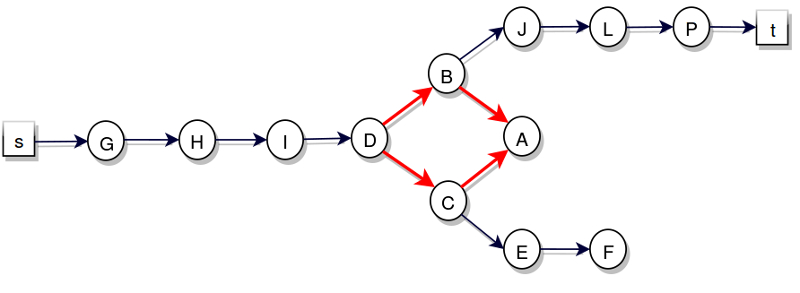
\includegraphics{definitions/D6.jpg}
        \end{adjustbox}
    }
\end{center}

\textbf{Caminos Aumentantes}

\textbf{$sGHI\overleftarrow{DB}JKLPt: 10$}

\textbf{Capacidades actualizadas}

$\begin{array}{llllll} \overrightarrow{sA}: \cancel{100}\cancel{20}\cancel{16}\cancel{6}0& \overrightarrow{AB}: \cancel{150}\cancel{70}\cancel{66} 60&\overrightarrow{BJ}: \cancel{100}90&\overrightarrow{DF}: \cancel{4} 0&\overrightarrow{Ht}: \cancel{10}0&\overrightarrow{KL}: \cancel{100}90\\ \overrightarrow{sC}: \cancel{50}0& \overrightarrow{AC}: \cancel{10}0&\overrightarrow{CD}: \cancel{50}\cancel{0}6&\overrightarrow{EF}: \cancel{100}\cancel{50}\cancel{40}34&\overrightarrow{HI}: \cancel{100}90&\overrightarrow{LP}: \cancel{100}90\\ \overrightarrow{sE}: \cancel{50}0& \overrightarrow{Bt}: \cancel{80}&\overrightarrow{CE}: \cancel{20}\cancel{10}4&\overrightarrow{Ft}: \cancel{70}\cancel{20}\cancel{16}\cancel{6}0 &\overrightarrow{ID}: \cancel{100}90&\overrightarrow{Pt}: \cancel{100}90\\ \overrightarrow{sG}: \cancel{100}\cancel{90}80& \overrightarrow{BD}: \cancel{100}\cancel{96}\cancel{90}100&\overrightarrow{Dt}: \cancel{50}0&\overrightarrow{GH}: \cancel{100}\cancel{90}80&\overrightarrow{JK}: \cancel{100}90&\\ \end{array}$

\subsubsection*{Paso 5}

\textbf{Network Auxiliar}

\begin{center}
\textbf{
    \begin{adjustbox}{max size={\textwidth}{\textheight}}
        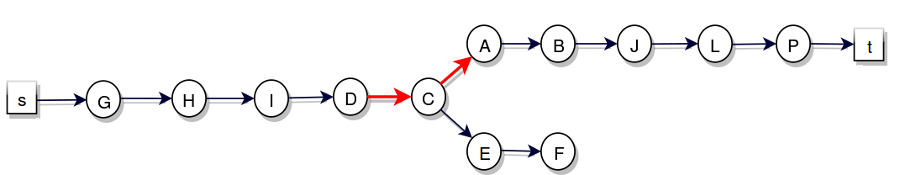
\includegraphics{definitions/D7.jpg}
        \end{adjustbox}
    }
\end{center}

\textbf{Caminos aumentantes}

\textbf{$sGHI\overleftarrow{DC}\overleftarrow{A}BJKLPt:10$}

\textbf{Capacidades actualizadas}

$\begin{array}{llllll} \overrightarrow{sA}: \cancel{100}\cancel{20}\cancel{16}\cancel{6}0& \overrightarrow{AB}: \cancel{150}\cancel{70}\cancel{66} \cancel{60}50&\overrightarrow{BJ}: \cancel{100}\cancel{90}80&\overrightarrow{DF}: \cancel{4} 0&\overrightarrow{Ht}: \cancel{10}0&\overrightarrow{KL}: \cancel{100}\cancel{90}80\\ \overrightarrow{sC}: \cancel{50}0& \overrightarrow{AC}: \cancel{10}\cancel{0}10&\overrightarrow{CD}: \cancel{50}\cancel{0}\cancel{6}16&\overrightarrow{EF}: \cancel{100}\cancel{50}\cancel{40}34&\overrightarrow{HI}: \cancel{100}\cancel{90}80&\overrightarrow{LP}: \cancel{100}\cancel{90}80\\ \overrightarrow{sE}: \cancel{50}0& \overrightarrow{Bt}: \cancel{80}&\overrightarrow{CE}: \cancel{20}\cancel{10}4&\overrightarrow{Ft}: \cancel{70}\cancel{20}\cancel{16}\cancel{6}0 &\overrightarrow{ID}: \cancel{100}\cancel{90}80&\overrightarrow{Pt}: \cancel{100}\cancel{90}80\\ \overrightarrow{sG}: \cancel{100}\cancel{90}\cancel{80}70& \overrightarrow{BD}: \cancel{100}\cancel{96}\cancel{90}100&\overrightarrow{Dt}: \cancel{50}0&\overrightarrow{GH}: \cancel{100}\cancel{90}\cancel{80}70&\overrightarrow{JK}: \cancel{100}\cancel{90}80&\\ \end{array}$

\subsubsection*{Paso 6}

\textbf{Network auxiliar}

\begin{center}
\textbf{
    \begin{adjustbox}{max size={\textwidth}{\textheight}}
        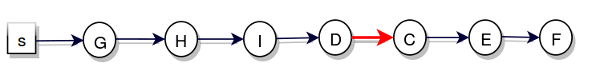
\includegraphics{definitions/D8.jpg}
        \end{adjustbox}
    }
\end{center}

Como no llegamos a $t$, esto es, no existen caminos aumentantes entre $s$ y $t$, podemos afirmar que el flujo obtenido es maximal.

\textbf{Valor del flujo}

\textbf{$v(f_{MAX}) = f_{MAX} (\overrightarrow{sA}) + f_{MAX} (\overrightarrow{sC}) + f_{MAX} (\overrightarrow{sE}) + f_{MAX} (\overrightarrow{sG}) = 230$}

\textbf{Corte minimal}

\textbf{$S= \{s, G, H, I, D, C, E, F\}
$}

\textbf{$CAP(S) = C(S, V- S) = c(\overrightarrow{sA}) + c(\overrightarrow{Ht}) + c(\overrightarrow{Dt}) + c(\overrightarrow{Ft}) = 100 + 10 + 50 + 70 = 230$}

\section*{Correctitud Dinic}

En una corrida del algoritmo, sea $A$ un network auxiliar y sea $A'$ el siguiente network auxiliar. Sea $d(x)$ la distancia de $s$ a $x$ en $A$ y sea $d'(x)$ la distancia de $s$ a $x$ en $A'$. Entonces $d(t) < d'(t)$. Es decir, la distancia en networks auxiliares sucesivos aumenta.

\subsubsection*{Prueba}

Por la prueba de Edmonds-Karp, sabemos que $d(t) \leq d'(t)$, pero queremos probar $d(t) < d'(t)$, o sea, que es estrictamente menor.

Sea $s=x_0, x_1, x_2,\dots, x_r=t$ un camino dirigido en $A'$. Afirmamos que ese camino \textbf{no existe} en $A$, pues para pasar de $A$ a $A'$ debimos bloquear todos los caminos dirigidos de $A$. Por lo tanto, si ese camino hubiese estado en $A$, Dinic lo habría bloqueado y por lo tanto no estaría en $A'$. Veamos cuáles son las posibles razones de que ese camino no esté en $A$.

\begin{enumerate}

	\item Falta un vértice, es decir, $\exists\;i$ tal que $x_i\not\in V(A)$
	\item Falta un lado, es decir, $\exists\;i$ tal que $\overrightarrow{x_ix_{i+1}} \not \in E(A) $
	\begin{enumerate}

		\item $\overrightarrow{x_ix_{i+1}}$ no está porque corresponde a un lado vacío o saturado en $N$ (ni siquiera está en el network residual)
		\item $\overrightarrow{x_ix_{i+1}}$ está en el network residual, pero $d(\overrightarrow{x_{i+1}})\neq d(x_i) + 1$
	\end{enumerate}
	
\end{enumerate}

Analicemos los tres casos

1) Si $x_i\not\in V(A)$, entonces

\begin{center}
\begin{align*}
d(t) &\leq d(x_i)\quad\quad\text{(por eso lo excluimos de } A\text{)}\\
&\leq d'(x_i)\quad\quad \text{(por prueba Edmonds-Karp)}\\
&< d'(t) \quad\quad\text{(ya que }t\text{ esta despues en este camino}\\
\end{align*}
\end{center}

2.a) $\overrightarrow{x_ix_{i+1}}$ no está siquiera en el network residual que da origen a $A$. Pero necesariamente debe estar en el que da origen a $A'$. Para que pase esto, debemos haber utilizado en $A$ el lado $\overrightarrow{x_{i+1}x_{i}}$. Por la prueba de Edmonds-Karp, sabemos que entonces

\begin{center}
$d'(t) \geq d(t) + 2 > d(t)$
\end{center}

2.b) $\overrightarrow{x_ix_{i+1}}$ está en el network residual que da origen a $A$, debe ser $d(\overrightarrow{x_{i+1}})\leq d(x_i) + 1$ (mayor no puede ser, ya que al estar conectado $x_{i}$ con $x_{i+1}$, la distancia es mayor en a lo sumo una unidad) pero como no está en $A$, debe ser $d(\overrightarrow{x_{i+1}})\neq d(x_i) + 1$. Concluimos que $d(\overrightarrow{x_{i+1}})< d(x_i) + 1$ (*). Entonces:

\begin{center}
\begin{align*}
d(t) &= d(x_{i+1}) + b(x_{i+1})\quad \quad \text{(ver prueba EK)}\\
&\leq d(x_{i+1})+b'(x_{i+1})\quad \quad \text{(ver prueba EK)}\\
&< d(x_i)+1+b'(x_{i+1})\quad \quad \text{(por (*))}\\
&\leq d'(x_i)+1+b'(x_{i+1})\quad \quad \text{(ver prueba EK)}\\
&\leq d'(t)
\end{align*}
\end{center}

Esta prueba nos dice que los caminos aumentantes provistos por networks auxiliares sucesivos deben ser cada vez más largos. En consecuencia, alguna vez deja de haber caminos aumentantes (ya que el número de vértices en el grafo es finito).

\section*{Complejidad de Dinic}

La complejidad de Dinic es $O(n^2m)$, lo cual es un avance con respecto a Edmons-Karp que se nota para grafos dendos (donde $m$ es del orden de $n^2$).

\subsubsection*{Prueba}

Vimos que la distancia en networks auxiliares sucesivos aumenta. Como la distancia entre $s$ y $t$ puede ir desde $1$ hasta $n -1$, hay a lo sumo $O(n)$ networks auxiliares.

\begin{center}
Complejidad de Dinic $= O(n)\cdot $ complejidad de hallar flujo bloqueante en $NA$
\end{center}

Por lo tanto, tenemos que probar que esto último está en $O(nm)$.

Para hallar un flujo bloqueante, debemos

\begin{enumerate}

	\item Crear $NA$, que se hace con BFS, que es $O(m)$
	\item Hallar flujo bloqueante
\end{enumerate}

En el pseudocódigo presentado para este algoritmo, hay secciones indicadas como AVANZAR, RETROCEDER e INCREMENTAR. Llamaremos:

\begin{itemize}

	\item AVANZAR $\rightarrow$ $A$
	\item RETROCEDER $\rightarrow$ $R$
	\item INCREMENTAR $\rightarrow$ $I$
\end{itemize}

La búsqueda del flujo bloqueante de Dinic luce como una palabra con estos tres símbolos:

\begin{center}
$AAAIAAAAAIAR\dots AIARAAI\dots$
\end{center}

Es una palabra cuyo alfabeto es $\{A, I, R\}$. Subdividamos las posibles palabras en

\begin{itemize}

	\item $A^+I$
	\item $A^+R$
	\item $R$ (puede haber $R$ sin $A$ antes).
\end{itemize}

Debemos calcular la complejidad de cada palabra, y la cantidad de cada una.

Recordemos:

$A$:


    \lstset{
        commentstyle=\color{mygreen},
        keywordstyle=\color{myred},
        frame=single,
        backgroundcolor=\color{gray!10},
        inputencoding=utf8,
        extendedchars=true,
        mathescape=true,
        breaklines=true,
        literate={á}{{\'a}}1 {é}{{\'e}}1 {í}{{\'i}}1 {ó}{{\'o}}1 {ú}{{\'u}}1 {ñ}{{\~n}}1
    }
    \begin{lstlisting}[language=pseudo]
// AVANZAR
P[i+1] = algún vértice en $\Gamma^+($P[i]$)$
i++;
// FIN AVANZAR
\end{lstlisting}

tiene complejidad $O(1)$

$R$:


    \lstset{
        commentstyle=\color{mygreen},
        keywordstyle=\color{myred},
        frame=single,
        backgroundcolor=\color{gray!10},
        inputencoding=utf8,
        extendedchars=true,
        mathescape=true,
        breaklines=true,
        literate={á}{{\'a}}1 {é}{{\'e}}1 {í}{{\'i}}1 {ó}{{\'o}}1 {ú}{{\'u}}1 {ñ}{{\~n}}1
    }
    \begin{lstlisting}[language=pseudo]
// RETROCEDER
Borrar P[i-1]P[i] del NA
i--;
// FIN RETROCEDER
\end{lstlisting}

Tiene complejidad $O(1)$

$I$:


    \lstset{
        commentstyle=\color{mygreen},
        keywordstyle=\color{myred},
        frame=single,
        backgroundcolor=\color{gray!10},
        inputencoding=utf8,
        extendedchars=true,
        mathescape=true,
        breaklines=true,
        literate={á}{{\'a}}1 {é}{{\'e}}1 {í}{{\'i}}1 {ó}{{\'o}}1 {ú}{{\'u}}1 {ñ}{{\~n}}1
    }
    \begin{lstlisting}[language=pseudo]
// INCREMENTAR
$\varepsilon = \min\{c($P[i]P[i+1]$)-g($P[i]P[i+1]$) \;\forall \; 0 \leq i \leq d\}$
for i= 0 to d -1:
    g+= $\varepsilon$
    if $g($P[i]P[i+1]$)$ = $c($P[i]P[i+1]$)$:
        borrar lado P[i]P[i+1] del NA
// FIN INCREMENTAR
\end{lstlisting}

Recorre un camino de longitud $d(t)$ 2 veces, por lo tanto, tiene complejidad $O(d)$.

Por lo tanto, la complejidad de las palabras de tipo $A^+R$  es $O(j)$, donde $j$ es la cantidad de veces que se repite la letra $A$. Pero cada $A$ incrementa $i$, y tenemos $0 \leq i \leq d$, por lo tanto $j\leq d$. Concluimos que la complejidad de este tipo de palabras está en $O(d)$.

Por un razonamiento análogo (no puede haber más de $d$ letras $A$), la complejidad de las palabras de tipo $A^+I$ es $O(d) + O(d) = O(d)$.

Por último, $R$ tiene la instrucción "borrar lado", por lo que puede haber a lo sumo $m$ palabras de tipo $A^+R$, y también $I$ tiene la instrucción oculta (que se ejecuta al menos una vez) de "borrar lado". Luego, el número de veces que hay palabra de tipo $A^+I$ debe ser como máximo $m$. Por lo tanto, hay a lo sumo $m$ palabras de cada tipo.

La complejidad de "hallar camino bloqueante es" $O(m) + O(md) = O(md)$. Pero como $d\leq n$, podemos decir que la complejidad de Dinic es $O(mn^2)$.

 

\section*{Estrategias de resolución de problemas}

Hemos visto problemas (2-color, max-flox/min cut) que se sesuelven con algoritmos polinomiales determinísticos y otros para los cuales no se conoce un algoritmo polinomial que los resuelva (3-color, calcular $\chi(G)$). ¿Qué hacemos con estos problemas?

Existen algoritmos que mediante algo de aleatoriedad intentan alcanzar una solución aceptable (no necesariamente la óptima).

\subsubsection*{Estrategias básicas}

\begin{enumerate}

	\item Exploration: búsqueda más o menos ciega del espacio de solución (ej: seleccionar órden de vértices al azar y correr coloreo greedy a ver si obtenemos un coloreo con menos colores que el que ya tenemos).
	\item Explotation: búsqueda dirigida utilizando alguna propiedad del problema que se conoce (ej: greedy con un orden específico no empeora el coloreo que se tiene).
\end{enumerate}

El problema con la exploración guiada puede ser que converja a un mínimo local (o máximo) y no encuentre el mínimo (o máximo).

Ejemplos de estrategias dirigidas:

HILL CLIMBING: modifica aleatoriamente la solución actual y se queda con la nueva sólo sí es menor o igual a la anterior.

SIMULATED ANNEALING: Igual que Hill Climbing, pero una solución peor se puede aceptar de acuerdo a determinada probabilidad.

\section*{Algoritmos genéticos}

Características

\begin{enumerate}

	\item trabajan sobre poblaciones (de soluciones)
	\item Los individuos (soluciones) interactúan entre sí
	\item Trata de imitar la selección natural
\end{enumerate}

Tienen 3 operadores básicos:

\subsubsection*{Mutación}

Cambia aleatoriamente a un individuo, con baja probabilidad y su función es "explorar" el espacio de soluciones. Permite salir de mínimos (o máximos) locales. Se regula mediante probabilidades.

\subsubsection*{Crossover}

Imita el crossover real de la reproducción de las especies. Básicamente, a partir de dos invididuos de la vieja población se obtienen dos individuos de la nueva generación (la población es estable, no aumenta ni decrece de una generación a la siguiente).

\subsubsection*{Selección}

Es la decisión de qué parejas van a ser sometidas al crossover (simulando la reproducción, para avanzar a la siguiente generación). Algunos individuos serán seleccionados más de una vez; otros, por lo tanto, ninguna.

Esquema básico de algoritmos genéticos


    \lstset{
        commentstyle=\color{mygreen},
        keywordstyle=\color{myred},
        frame=single,
        backgroundcolor=\color{gray!10},
        inputencoding=utf8,
        extendedchars=true,
        mathescape=true,
        breaklines=true,
        literate={á}{{\'a}}1 {é}{{\'e}}1 {í}{{\'i}}1 {ó}{{\'o}}1 {ú}{{\'u}}1 {ñ}{{\~n}}1
    }
    \begin{lstlisting}[language=pseudo]
t = 0
crear aleatoriamente una población inicial P(0)
while (no se den las condiciones para parar):
    selección (P(t))
    crossover
    mutación
    P(t+1) = Población así obtenida
    t++
\end{lstlisting}

\section*{Crossover}

Es el mecanismo mediante el cual a partir de dos individuos de la población $t$ se obtienen dos individuos de la población $t+1$.

\subsubsection*{Crossover simple}

Imita el crossover de la vida real. El "cromosoma" se corta en un sólo punto. Ej:

\begin{center}
$\begin{array}{cccccc|cccccc} P_1 &= &\color{green} A&\color{green}C&\color{green}G&\color{green}T&\color{green}F&\color{green}R&\color{green}G&\color{green}A&\color{green}D&\color{green}E\\ P_2 &= & \color{blue}B&\color{blue}E&\color{blue}F&\color{blue}C&\color{blue}K&\color{blue}E&\color{blue}R&\color{blue}A&\color{blue}B&\color{blue}C\\ \end{array} \Rightarrow \begin{array}{cccccc|cccccc} H_1 &= &\color{green} A&\color{green}C&\color{green}G&\color{green}T&\color{blue}K&\color{blue}E&\color{blue}R&\color{blue}A&\color{blue}B&\color{blue}C\\ H_2 &= & \color{blue}B&\color{blue}E&\color{blue}F&\color{blue}C&\color{green}F&\color{green}R&\color{green}G&\color{green}A&\color{green}D&\color{green}E\\ \end{array}$
\end{center}

\subsubsection*{Two point crossover}

El cromosoma se corta en dos puntos:

\begin{center}
$\begin{array}{ccc|cccc|ccccc} P_1 &= &\color{green} A&\color{green}C&\color{green}G&\color{green}T&\color{green}F&\color{green}R&\color{green}G&\color{green}A&\color{green}D&\color{green}E\\ P_2 &= & \color{blue}B&\color{blue}E&\color{blue}F&\color{blue}C&\color{blue}K&\color{blue}E&\color{blue}R&\color{blue}A&\color{blue}B&\color{blue}C\\ \end{array} \Rightarrow \begin{array}{ccc|cccc|ccccc} P_1 &= &\color{green} A&\color{blue}E&\color{blue}F&\color{blue}C&\color{blue}K&\color{green}R&\color{green}G&\color{green}A&\color{green}D&\color{green}E\\ P_2 &= & \color{blue}B&\color{green}C&\color{green}G&\color{green}T&\color{green}F&\color{blue}E&\color{blue}R&\color{blue}A&\color{blue}B&\color{blue}C\\ \end{array}$
\end{center}

\subsubsection*{Order based crossover}

Comenzamos trazando una línea como en el crossover simple

\begin{center}
$\begin{array}{cccccc|cccccc} P_1 &= &A&B&C&D&E&F&G&H&I&J\\ P_2 &= & B&E&F&C&J&I&D&G&A&H\\ \end{array}$
\end{center}

Luego para obtener el hijos $H_1$ se toma la primera parte del progenitor $P_1$ y la segunda se reordena según el orden que dicta $P_2$ y viceversa:

\begin{center}
$\begin{array}{cccccc|cccccc} H_1 &= &A&B&C&D&E&F&J&I&G&H\\ H_2 &= & B&E&F&C&A&D&G&H&I&J\\ \end{array}$
\end{center}

\subsubsection*{Cyclic Crossover}

Dado dos progenitores de la forma

\begin{center}
$\begin{array}{cccccccccccc} P_1 &= &B&I&G&A&E&C&J&F&D&H\\ P_2 &= &D&J&B&F&E&C&I&G&A&H\\ \end{array}$
\end{center}

obtenemos el hijo $H_1$ por pasos a partir de $P_2$ del siguiente modo:

\begin{enumerate}

	\item $ \begin{array}{cccccccccccccc} H_1 &= &P_2 &=&D&J&B&F&E&C&I&G&A&H\\ \end{array}$
	\item Elegimos un elemento al azar, en este caso el primero, y lo cambiamos por el elemento en esa posición de $P_1 $,
	\item $ \begin{array}{cccccccccccc} H_1 &=&\cancel{D}&J&B&F&E&C&I&G&A&H\\ & & B &&&&&&&&& \end{array}$
	\item Para evitar que haya dos $B$ repetidas, cambiamos la otra $B$ por el elemento en esa posición de $P_1$,
	\item $ \begin{array}{cccccccccccc} H_1 &=&\cancel{D}&J&\cancel{B}&F&E&C&I&G&A&H\\ & & B &&G&&&&&&& \end{array}$
	\item etc.
\end{enumerate}

Si hay ciclos de $1$ o de $n$ elementos, no habrá cambios.

\subsubsection*{PMX}

Partial mixing crossover, es similar a two-point crossover, con distinta técnica.

Primero se selecciona un bloque al azar.

\begin{center}
$\begin{array}{cccc|cccc|c}
P_1 &= &A&B&C&D&E&F&G\\
P_2 &= &E&D&F&G&B&A&C\\
\end{array}$
\end{center}

Se intercambian:

\begin{center}
$\begin{array}{cccc|cccc|c}
H_1 &= &A&B&F&G&B&A&G\\
H_2 &= &E&D&C&D&E&F&C\\
\end{array}$
\end{center}

Se crea una tabla de equivalencias a partir de los elementos del bloque central:

\begin{center}
\begin{align*}
A &\leftrightarrow F \leftrightarrow C\\
D&\leftrightarrow  G\\
B&\leftrightarrow  E \\
\end{align*}
\end{center}

Se utiliza la tabla de equivalencias para obtener los reemplazos adecuados para los elementos fuera del bloque central:

\begin{center}
$\begin{array}{cccc|cccc|c}
        &    & C&E&&&&&D\\
H_1 &= &\cancel{A}&\cancel{B}&F&G&B&A&\cancel{G}\\
H_2 &= &\cancel{E}&\cancel{D}&C&D&E&F&\cancel{C}\\
        &    & B&G&&&&&A\\
\end{array}$
\end{center}

 

\section*{Selección}

Se requiere una fitness function (función de adaptabilidad). A mayor valor de fitness, mayor será la probabilidad de un individuo de ser seleccionado para su reproducción. A partir del valor de esta función, se calcula la "esperanza de reproducción", que transforma el valor de adaptabilidad en una probablidad de reproducción, o bien cuántes veces espera el individuo reproducirse.

\begin{center}
$E_i = \frac{F(i)}{\overline{F}}$,
\end{center}

donde $\overline{F} =\frac{\sum\limits_{i} F(i)}{n}$ es el promedio de los valores que toma la función de fitness en el conjunto de todos los individuos.

Usando los valores de $E_i$ seleccionamos los individuos para hacer crossover.

Por ejemplo:

\begin{center}
$\begin{array}{c|r} F(1) & 17,118\\ F(2) &9,51\\ F(3) &36,138\\ F(4) &22,824\\ F(5)&91,926\\ F(6)&13,314\\ \end{array}$
\end{center}

Se tiene que $\sum\limits_{i}F(i) = 190,2$ y $\overline{F} = 31, 7$, por lo tanto:

\begin{center}
$\begin{array}{c|r} E(1) &0,54\\ E(2) & 0,3\\ E(3) & 1,14\\ E(4) & 0,72\\ E(5)& 2,88\\ E(6)& 0,42\\ \end{array}$
\end{center}

Se puede decir que el individuo $1$ tiene una esperanza de reproducirse entre $0$ y $1$ vez, mientras que el individuo $5$ puede esperar reproducirse entre $2$ y $3$ veces.

A continuación se detallan algunos métodos para elegir los individuos (y las parejas respectivas) que se utilizarán para la reproducción, a partir de las esperanzas de reproducción calculadas.

\subsubsection*{Ruleta}

Elegir $2$ individuos al azar de entre los $6$ (tres veces, en total) usando $E_i$ como peso, os ea, el individo $5$ tiene más chances de salir seleccionado. Un método común es como sigue:

\begin{enumerate}

	\item Seleccionar $n$ números al azar, entre $0$ y $n$ (por ejemplo, $4,2;\; 0,9;\;1,32;\;2,76;\;3,78;\;4,98$)
	\item Para cada número, elegir el primer $i$ tal que $\sum\limits_{j\leq i}E_j \geq$ número (la suma de las esperanzas acumuladas hasta ese individuo).
\end{enumerate}

\begin{center}
$\begin{array}{c|r|r} i & E(i) &\sum\limits_{j\leq i}E_j\\ \hline 1 &0,56 & 0,54\\ 2 & 0,3 & 0,84\\ 3 & 1,14 & 1,98\\ 4 & 0,72 & 2,7\\ 5& 2,88 &5,58\\ 6& 0,42& 6\\ \end{array}$
\end{center}

De este modo,

\begin{itemize}

	\item $4,2$ nos dice que elijamos al individuo $5$,
	\item $0,9$ nos dice que elijamos al individuo $3$, (esta es la primer pareja)
	\item $1,32$ nos dice que elijamos al individuo $3 $,
	\item $2,76$ nos dice que elijamos al individuo $5$ (esta es la segunda pareja)
	\item $3,78$ nos dice que elijamos al individuo $5$
	\item $4,98$ nos dice que elijamos al individuo $5$ (esta es la tercer pareja)
\end{itemize}

\subsubsection*{SUS (Stochastic Universal Sampling)}

Elegir un número al azar entre $0$ y $1$. El resto es como el método \textbf{Ruleta}, pero los números que se usan para delimitar los intervalos son

\begin{center}
$x;\;x+1;\;x+2;\;\dots ;\; x+n-1$
\end{center}

Ejemplo: número al azar $x=0,3$,

\begin{center}
$\begin{array}{cccccc} 0,3&1,3&2,3&3,3&4,3&5,3\\ I_1&I_3&I_4&I_5&I_5&I_5 \end{array}$
\end{center}

De acuerdo a este método, tendríamos las parejas $(I_1; I_3), (I_4; I_5), (I_5;I_5)$

\subsubsection*{Métodos con remainder (resto)}

Para cada $i$, asignamos al individuo $I_i$ $\lfloor{E_i}\rfloor$ "tokens" de reproducción:

\begin{center}
$\begin{array}{ccccc} I_1 &\rightarrow &\lfloor E_i\rfloor = \lfloor 0,54\rfloor& \rightarrow & 0\\ I_2 & \rightarrow & \rightarrow &\rightarrow &0\\ I_3 & \rightarrow & \rightarrow &\rightarrow &1\\ I_4 & \rightarrow & \rightarrow &\rightarrow &0\\ I_5 & \rightarrow & \rightarrow &\rightarrow &2\\ I_6 & \rightarrow & \rightarrow &\rightarrow &0\\ \end{array}$
\end{center}

Según esto, el individuo $I_3$ tiene garantizada una "plaza" de reproducción, mientras que el individuo $I_5$, a su vez tiene dos. Quedan entonces tres plazas de reproducción por asignar, entonces, aplicamos \textbf{Ruleta} o \textbf{SUS} a sus restos:

\begin{center}
$\begin{array}{c|r|r} &&\sum\limits_{i}\\ R_{I_1} & 0,54 & 0,54\\ R_{I_2} & 0,3 & 0,84\\ R_{I_3} & 0,14 & 0,98\\ R_{I_4} & 0,72 & 1,71\\ R_{I_5} & 0,88 & 2,58\\ R_{I_6} & 0,42& 3\\ \end{array}$
\end{center}

Seleccionamos $3$ números entre $0$ y $3 $, etc.

\subsubsection*{Métodos basados en el ranking}

Sólo dependen de la posición del individuo en el ranking y no del valor concreto de la función fitness. En nuestro ejemplo, el ranking sería:

\begin{center}
$I_5, I_3, I_4, I_1, I_6, I_2$
\end{center}

Una manera de determinar la esperanza de cada individuo a partir de su posición es

\begin{center}
$LP(P) = (2-Sp) + 2(Sp-1) \cdot \frac{P-1}{n-1}$, con $1 \leq Sp \leq 2$,
\end{center}

Donde $P=n- \text{posicion} + 1$, $Sp$ es un parámetro (Selection pressure).

Ejemplo, con $Sp = 2$

\begin{center}
\begin{align*} I_2&\rightarrow LP(1) = 0\\ I_6&\rightarrow LP(2) = 0,4\\ I_1&\rightarrow LP(3) = 0,8\\ I_4&\rightarrow LP(4) = 1,2\\ I_4&\rightarrow LP(5) = 1,6\\ I_5&\rightarrow LP(6) = 2\\ \end{align*}
\end{center}

(Luego aplicar \textbf{Ruleta} o \textbf{SUS} con esos valores)

\textbf{Forma 2:}

Este método previene el problema de la early convergence. Cambia la forma de calcular $E_i$ tomando $E_i^*$ (sigma scaling).

\begin{center}
$E_i^* = 1 + \frac{F_i - \overline{F}}{2\sigma} $
\end{center}

donde $\sigma$ es la desviación estándar de los $F_i$.

En nuestro ejempplo, tenemos $\sigma = 30,637$ y $2\sigma = 61,27$, con lo que

\begin{center}
\begin{align*} E^*_1 &= 1 +\frac{ 17, 118 - 31,7}{61,27} = 0,762\\ E^*_2 &= 0,638\\ E^*_3 &= 1,0724\\ E^*_4 &= 0,855\\ E^*_5 &= 1,9726\\ E^*_6 &= 0,6939\\ \end{align*}
\end{center}

Esto tiene el efecto de achicar las diferencias entre las esperanzas. Luego, aplicar uno de los métodos anteriores con estos valores.

 

\section*{Matching}

Dado un grafo $G$, un matching en $G$ es un subgrafo $M$ de $G$ tal que

\begin{center}
$d_M(x) = 1\quad \forall\;x \in V(M)$
\end{center}

Es decir, el grado (relativo al subgrafo $M$) de $x$ es $1$ para todos los vértices de $M$.

Ejemplo:

\begin{center}

    \begin{adjustbox}{max size={\textwidth}{\textheight}}
        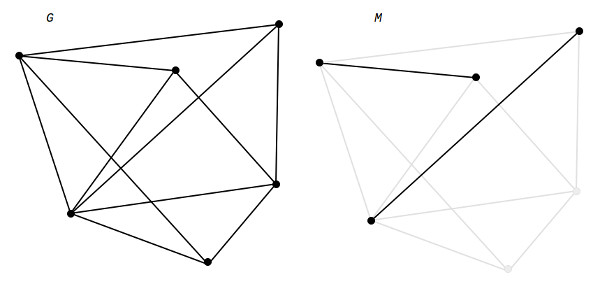
\includegraphics{definitions/matching_1.jpg}
        \end{adjustbox}
    
\end{center}

\section*{Matching maximal}

Un matching $M$ es maximal en $G$ si

\begin{center}
$\lvert E(M)\rvert \geq \lvert E(M')\rvert\quad \forall\; M'\text{ matching en } G$
\end{center}

Es decir, la cardinalidad del conjunto de lados del matching $M$ es la máxima posible.

De ahora en adelante, restringiremos nuestra atención al problema de encontrar matching maximal en grafos bipartitos.

\section*{Matching maximal como un problema de Max-Flow / Min-Cut}

Daremos un algoritmo para encontrar un matching maximal en un grafo \textbf{bipartito}.

\subsubsection*{Notación}

Cuando escribimos $G = (X \cup Y, E)$ queremos significar que $X$ e $Y$ son las dos partes de $V(G)$ tales que $X\cap Y = \emptyset$ y $X \cup Y = V(G)$.

\subsubsection*{Algoritmo}

Dado $G = (X \cup Y, E)$ bipartito, entonces construimos $N = N(G) $ un network con

\begin{center}
\begin{align*} V(N) &= V(G) \cup \{s, t\}\\ E(N) &= \{\overrightarrow{xy}: x\in X, y \in Y, \overrightarrow{xy} \in E(G)\} \cup \{\overrightarrow{sx}:x\in X\} \cup \{\overrightarrow{yt}:y\in Y\} \end{align*}
\end{center}

Con capacidades en todos los lados igual a $1$.

Con $G$ construido de esta manera, buscamos un flujo maximal $f$.

A partir de $f$, construimos el matching $M_f$ en $G$ de la siguiente manera:

\begin{center}
\begin{align*} V(M_f) &= \{x\in X : \exists \;y \in Y : f(\overrightarrow{xy}) = 1\} \cup \{y \in Y : \exists \;x \in X : f(\overrightarrow{xy}) = 1\}\\ E(M_f) &= \{xy: x \in X, y \in Y, f(\overrightarrow{xy}) = 1\} \end{align*}
\end{center}

Entonces, como se ve en el diagrama a continuación:

\begin{center}

    \begin{adjustbox}{max size={\textwidth}{\textheight}}
        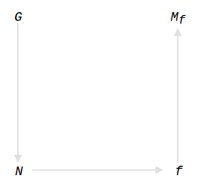
\includegraphics{definitions/matching_2.jpg}
        \end{adjustbox}
    
\end{center}

recibimos un grafo $G$, lo utilizamos para obtener un network $N$, calculamos un flujo maximal $f$ en $N$, utilizamos $f$ y $N$ para construir un matching $M_f$ en $G$. Debemos probar ahora que $M_f$ es matching y que es maximal.

\subsubsection*{$M_f$ es matching}

Si no lo fuera, existiría $z\in V(M_f)$ tal que $d_{M_f}(z) = 0$ o $d_{M_f}(z) \geq 2$. Lo primero es imposible, porque por construcción, sólo se agregan a $M_f$ aquellos vértices que están conectados con algo.

Veamos lo segundo.

Si $z \in X$: como $d_{M_f}(z) \geq 2$, entonces $\exists \;y_1, y_2 \in Y$ distintos tales que $zy_1, zy_2\in E(M_f)$. Pero entonces

\begin{center}
$f(\overrightarrow{zy_1}) = f(\overrightarrow{zy_2}) = 1 \Rightarrow OUT_f(z) \geq 2 $,
\end{center}

mientras que

\begin{center}
$\Gamma^-(z) = \{s\} \Rightarrow IN_f(z) \leq 1$,
\end{center}

lo cual es imposible.

Si $z \in Y$: mediante un razonamiento análogo pero con $t$ en lugar de $s$, veríamos que no se cumple la conservación y $f$ no sería flujo, lo cual es absurdo.

\subsubsection*{Biyección entre flujos $f$ y matchings $M_f$}

Observermos que

\begin{center}
\begin{align*} v(f) &= \sum\limits_{x\in X} f(\overrightarrow{sx})\\ &=\lvert \{x\in X: f(\overrightarrow{sx}) = 1\}\rvert\\ &= \lvert V(M_f) \cap X\rvert\quad\text{ pues }M_f\text{ es matching y } G \text{ es bipartito}\\ &= \lvert E(M_f)\rvert \end{align*}
\end{center}

es decir que el valor del flujo $f$ (que es maximal) coincide con el número de lados en el matching.

Viceversa, dado un matching en $G$, el flujo $f_M$ dado por

\begin{center}
$f_M (\overrightarrow{xy})= \begin{cases} 1 & xy \in E(M)\\ 0 & xy \not \in E(M) \end{cases}$
\end{center}

\begin{center}
$f_M (\overrightarrow{sx})= \begin{cases} 1 & x \in V(M)\\ 0 & x \not \in V(M) \end{cases}$
\end{center}

\begin{center}
$f_M (\overrightarrow{yt})= \begin{cases} 1 & y \in V(M)\\ 0 & y \not \in V(M) \end{cases}$
\end{center}

efectivamente es flujo, pues

\begin{center}
\begin{align*} x\not \in V(M) &\Rightarrow f_M(\overrightarrow{sx}) = 0, f_M(\overrightarrow{xy}) = 0\quad \forall \; y\\ & \Rightarrow IN_f(x) = 0, OUT_f(x) = 0 \end{align*}
\end{center}

\begin{center}
\begin{align*} x \in V(M) &\Rightarrow f_M(\overrightarrow{sx})=1\\ &\Rightarrow IN_f(x) = 1\\ &\Rightarrow \exists \; y \text{ unico tal que } f(\overrightarrow{xy}) = 1\\ &\Rightarrow OUT_f(x) = 1 = IN_f(x)\\ \end{align*}
\end{center}

y de forma análoga, si $y \in Y$ se puede demostrar que $IN_f(y) = OUT_f(y)$.

Además está claro por la definición, $M_{f_M} = M$. Entonces $v(f_M) = \lvert E(M_{f_M})\rvert = \lvert E(M_f)\rvert$.

Todo esto sirvió para probar que tenemos una biyección entre los flujos maximales y los matchings construidos a partir de ellos.

\subsubsection*{$M_f$ es maximal}

Sea $f_{MAX}$ flujo maximal entero y $M_{f_{MAX}}$ matching construido a partir de este. Sea $M$ otro matching cualquiera. Entonces

\begin{center}
$\lvert E(M)\rvert = v(f_M) \leq v(f_{MAX}) = \lvert E(M_{f_{MAX}})\rvert$
\end{center}

es decir, $M_{f_{MAX}}$ es maximal.

\section*{Algoritmo para encontrar matching maximal}

\subsubsection*{Overview}

\begin{enumerate}

	\item Dinic con un network auxiliar (lo cual va a dar caminos de la forma $sx_1y_1t: 1\quad sx_2y_2t: 1\quad \dots\quad sx_ny_nt: 1$, que se corresponde a agregar estos lados al matching).
	\item Tras encontrar el primer flujo bloqueante con Dinic, continuar con Edmonds-Karp.
\end{enumerate}

\subsubsection*{Detalles}

Si tenemos que encontrar un matching maximal en el grafo $G$ dado por

\begin{center}

    \begin{adjustbox}{max size={\textwidth}{\textheight}}
        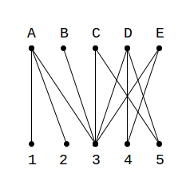
\includegraphics{definitions/matching_3.jpg}
        \end{adjustbox}
    
\end{center}

a partir del cual construimos el network $N$ dado por

\begin{center}

    \begin{adjustbox}{max size={\textwidth}{\textheight}}
        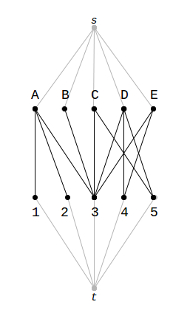
\includegraphics{definitions/matching_4.jpg}
        \end{adjustbox}
    
\end{center}

entonces podemos pensar en la matriz de adyacencia de $G$, que es de la forma

\begin{center}

    \begin{adjustbox}{max size={\textwidth}{\textheight}}
        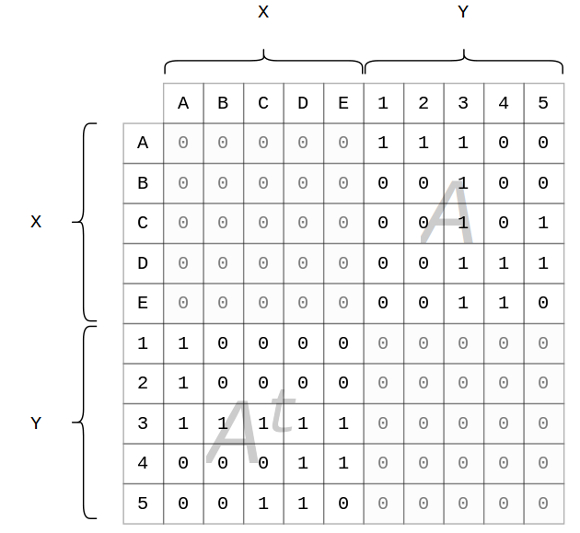
\includegraphics{definitions/matching_5.jpg}
        \end{adjustbox}
    
\end{center}

Observamos que por ser $G = (X \cup Y, E)$ un grafo bipartito, no hay unos en dos regiones importantes de la matriz. Estamos interesados entonces en la matriz $A$ que nos dice qué vértcies de $X$ se pueden unir con qué vértices de $Y$:

\begin{center}

    \begin{adjustbox}{max size={\textwidth}{\textheight}}
        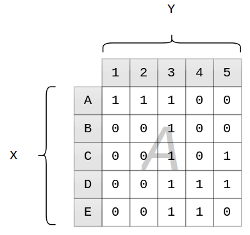
\includegraphics{definitions/matching_6.jpg}
        \end{adjustbox}
    
\end{center}

Es aquí donde corremos Dinic hasta encontrar un flujo bloqueante. Así, obtenemos los caminos:

\begin{center}
\begin{align*} &sA1t:1\\ &sB3t:1\\ &sC5t:1\\ &sD4t:1\\ \end{align*}
\end{center}

Lo cual equivale a agregar los lados $A1, B3, C5$ y $D4$ al matching:

\begin{center}

    \begin{adjustbox}{max size={\textwidth}{\textheight}}
        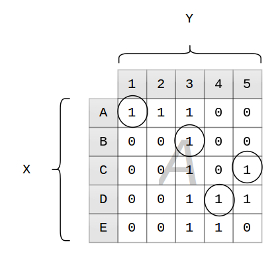
\includegraphics{definitions/matching_7.jpg}
        \end{adjustbox}
    
\end{center}

Luego aplicamos Edmonds-Karp, donde las colas van a ser de la forma:

\begin{center}
$\begin{array}{c|cccc|cccc|c|cccc|cc} s & x_{j_1} & x_{j_2} & \dots & x_{j_q} &y_{k_{11}}&y_{k_{12}} &\dots &y_{k_{1r}} &\dots&y_{k_{q1}}&y_{k_{q2}} &\dots &y_{k_{qr}} & \dots &\text{(lados backwards)}\\ & s & s & s & s & x_{j_1} & x_{j_1} &\dots & x_{j_1} &\dots& x_{j_q} & x_{j_q} &\dots & x_{j_q} & \\ \end{array}$
\end{center}

Es decir, donde

\begin{itemize}

	\item comenzamos con un grupo de vértices $x \in X$ agregados por $s$
	\item continuamos con vértices $y \in Y$ agregados por estos últimos
	\item los vértices de $Y$ comienzan a agregar vértices de $X$, nuevamente, como lados backwards,
	\item etc.
\end{itemize}

Esta cola la corremos manuamente colocando etiquetas al costado de la matriz $A$:

$s$ agrega a las filas no matcheadas, luego, etiquetamos dichas filas con $s$:

\begin{center}

    \begin{adjustbox}{max size={\textwidth}{\textheight}}
        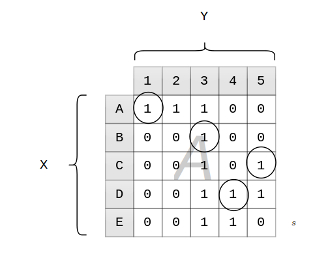
\includegraphics{definitions/matching_8.jpg}
        \end{adjustbox}
    
\end{center}

Lo cual sería como comenzar la cola de Edmonds-Karp con:

\begin{center}
$\begin{array}{cc} \cancel{s}& E \\ & s \end{array}$
\end{center}

Ahora es el turno de que $E$ incluya a los vértices de $Y$ que puede alcanzar y que no están en la cola, es decir, etiquetamos con $E$ las columnas correspondientes a vértices adyacentes a $E$ (allí donde hay unos) siempre y cuando no estén etiquetadas:

\begin{center}

    \begin{adjustbox}{max size={\textwidth}{\textheight}}
        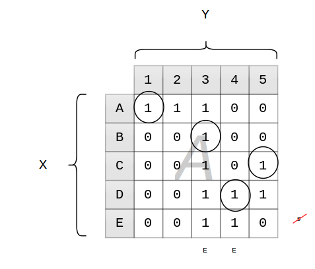
\includegraphics{definitions/matching_9.jpg}
        \end{adjustbox}
    
\end{center}

que es como haber continuado la cola de Edmonds-Karp del siguiente modo:

\begin{center}
$\begin{array}{cccc} \cancel{s}& \cancel{E} & 3 & 4 \\ & s & E & E \end{array}$
\end{center}

Como los elementos $3$ y $4$ (o, equivalentemente, las columnas $3$ y $4$) fueron previamente matcheadas, entonces pueden devolver flujo (lados backwards) a aquellos vértices de $X$ que se los enviaron que no están en la cola aún (o, equivalentemente, a las filas cuyos unos están marcados siempre que esas filas no hayan sido etiquetadas previamente):

\begin{center}

    \begin{adjustbox}{max size={\textwidth}{\textheight}}
        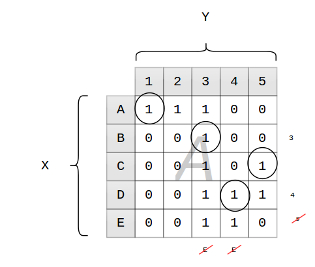
\includegraphics{definitions/matching_10.jpg}
        \end{adjustbox}
    
\end{center}

que es como haber continuado la cola de Edmonds-Karp así:

\begin{center}
$\begin{array}{cccccc} \cancel{s}& \cancel{E} & \cancel{3} & \cancel{4} & B & D \\ & s & E & E & 3^- & 4^- \end{array}$
\end{center}

Como $B$ no puede agregar elementos nuevos, simplemente lo tachamos. En cambio, la fila $D$ puede agregar a $5$:

\begin{center}

    \begin{adjustbox}{max size={\textwidth}{\textheight}}
        \includegraphics{definitions/matching_11.jpg}
        \end{adjustbox}
    
\end{center}

\begin{center}
$\begin{array}{ccccccc} \cancel{s}& \cancel{E} & \cancel{3} & \cancel{4} & \cancel{B} & \cancel{D} & 5\\ & s & E & E & 3^- & 4^- & D \end{array}$
\end{center}

Luego $5$ puede agregar $C$ (lado backwards):

\begin{center}

    \begin{adjustbox}{max size={\textwidth}{\textheight}}
        \includegraphics{definitions/matching_12.jpg}
        \end{adjustbox}
    
\end{center}

\begin{center}
$\begin{array}{cccccccc} \cancel{s}& \cancel{E} & \cancel{3} & \cancel{4} & \cancel{B} & \cancel{D} & \cancel{5} & C\\ & s & E & E & 3^- & 4^- & D & 5^- \end{array}$
\end{center}

Como $C$ ya no puede agregar a nadie y aún no pudimos llegar a $t$ (no etiquetamos ninguna columna sin matching) el matching no se puede exteneder. Luego, tenemos un matching maximal.

\section*{Matching Perfecto y Matching Completo}

Si $G = (X \cup Y, E)$ es bipartito diremos que un matching $M$ en $G$ es \textbf{perfecto} si $V(M) = V(G)$. Diremos que es \textbf{completo} de $X$ a $Y$ si $X\subseteq V(M)$ (o completo de $Y$ a $X$ si $Y \subseteq V(M)$).

\subsubsection*{Condiciones obvias}

Para que exista un matching perfecto, $\lvert X \rvert$ debe ser igual a $\lvert Y \rvert$ (de modo que pueda existir una biyección entre los elementos). Aún si $\lvert X \rvert = \lvert Y \rvert$ puede no haber matching perfecto (recordar ejemplo anterior).

\section*{$\Gamma(S)$ en un grafo}

Dado un grafo $G$ y un subconjunto $S \subseteq V(G)$,

\begin{center}
\begin{align*} \Gamma(S) &= \cup_{z \in S} \Gamma(z)\\ &= \{w \in V(G) : \exists \; z \in S : zw \in E(G)\} \end{align*}
\end{center}

Esta es la definición general, sin embargo en adelante nos vamos a restringir a casos con grafos bipartitos y con $S \subseteq X$ ó $S \subseteq Y$.

\section*{Teorema de Hall}

Sea $G = (X \cup Y, E)$ un grafo bipartito, entonces existe un matching completo de $X$ a $Y$ si y sólo si $\lvert S \rvert \leq \lvert \Gamma(S)\rvert$ para todo $S \subseteq X$.

\subsubsection*{Prueba}

$\Rightarrow$ Si $M$ es matching completo de $X$ a $Y$, entonces $\forall \; x \in X \;\exists!\; y \in Y: xy \in E(M)$. Sea

\begin{center}
$f(x) = $ ese único $y$
\end{center}

Notemos que entonces $f$ es una función inyectiva de $X $ a $Y$, ya que $xy\in M \land zy \in M \Rightarrow x = z$ (por ser $M$ un matching). Además, por definición $f(x) \in \Gamma(x)$. Esto implica que $f(S) \subseteq \Gamma(S) \; \forall \; S \subseteq X$ y por lo tanto $\lvert f(S)\rvert= \lvert S \rvert \leq \lvert \Gamma(S)\rvert$.

$\Leftarrow$ Supongamos que no es cierto. Entonces existe $G$ grafo bipartito con $\lvert S \rvert \leq \lvert \Gamma(S)\rvert\;\forall\;S \subseteq X$ pero no tiene matching completo de $X$ a $Y$. Esto quiere decir que cuando corremos el algoritmo, quedan filas sin matchear.

Sea $S_0$ el conjunto de tales filas y $T_1 = \Gamma(S_0)$. Todas las columnas de $T_1$ están matcheadas (pues si hubiera una libre, se matchearía con algo de $S_0$).

Sea $S_1 \subseteq X$ las filas matcheadas con las columnas de $T_1$ y sea $T_2 = \Gamma(S_1) - T_1$, etc.

En general:

\begin{center}
$S_i = $ Filas matcheadas por $T_i$
\end{center}

\begin{center}
$T_{i+1} = \Gamma(S_i) - (T_0 \cup T_1 \cup \dots \cup T_i)$
\end{center}

Esto puede continuar hasta que $T_n$ sea vacío, ya que $S_n$ no va a ser vacío nunca.

Como el algoritmo para sin hallar matching perfecto, y $\forall\;i$, $T_i \neq \emptyset$ produce un $S_i$, la única forma de parar es un $k$ tal que $T_{k+1} = \emptyset$.

Sea $S = S_0 \cup S_1 \cup \dots \cup S_k$ (las filas que tienen etiqueta).

Observaciones:

\begin{enumerate}

	\item Como $S_i$ son las filas matcheadas con $T_i$, entonces $\lvert S_i \rvert = \lvert T_i\rvert$ (por ser matching parcial).
	\item Por construcción, los $T_i$ son disjuntos
	\item $T_1 \cup T_2 \cup \dots \cup T_{i+1}= \Gamma(S_0 \cup S_1 \cup \dots \cup S_i)$
\end{enumerate}

\textbf{Prueba de }3: para $i = 1$ vale ($T_1 = \Gamma(S_0)$) , y si vale para $i$, entonces vale para $i + 1$, ya que:

\begin{center}
\begin{align*} T_1 \cup \dots \cup T_{i+2} &= T_1 \cup T_2 \cup \dots \cup T_{i+1} \cup T_{i+2}\\ &= T_1 \cup T_2 \cup \dots \cup T_{i+1} \cup(\Gamma(S_{i+1}) -( T_ 1 \cup \dots \cup T_{i+1}))\\ &= T_1 \cup T_2 \cup \dots \cup T_{i+1} \cup \Gamma(S_{i+1})\\ &= \Gamma(S_0 \cup S_1 \cup \dots \cup S_i) \cup \Gamma(S_{i+1})\\ &= \Gamma(S_0 \cup S_1 \cup \dots \cup S_i \cup S_{i+1})\\ \end{align*}
\end{center}

Entonces

\begin{center}
\begin{align*} \lvert \Gamma(S)\rvert &= \lvert \Gamma(S_0 \cup S_1 \cup \dots \cup S_k)\rvert\\ &= \lvert T_1 \cup T_2 \cup \dots \cup T_k \cup T_{k+1}\rvert \text{ (por 3)}\\ &= \lvert T_1 \cup T_2 \cup \dots \cup T_k\rvert \text{ (por }T_{k+1} = \emptyset\text{)}\\ &= \lvert T_1\rvert + \lvert T_2\rvert + \dots + \lvert T_k\rvert \text{ (por 2) }\\ &= \lvert S_1\rvert + \lvert S_2\rvert + \dots + \lvert S_k\rvert \text{ (por 1)}\\ &= \lvert S \rvert - \lvert S_0 \rvert\text{ (por 2)}\\ &< \lvert S \rvert \text{ (por ser } S_0 \neq \emptyset \text{)} \end{align*}
\end{center}

Esto contradice la hipótesis, es absurdo.

\subsubsection*{Aplicación}

A la hora de buscar un matching perfecto, si no lo encontramos, el teorema de Hall provee una manera de certificar que no existe:

\begin{center}
$S = $ Todas las filas marcadas
\end{center}

\begin{center}
$\Gamma(S) = $ todas las columnas marcadas
\end{center}

 

\section*{Teorema del matrimonio}

Todo grafo bipartito regular tiene un matching perfecto.

\subsubsection*{Estructura de la prueba}

\begin{enumerate}

	\item Probar que en un grafo bipartito regular todo matching completo es perfecto.
	\item Probar que en un grafo bipartito regular se cumple la condición de Hall.
\end{enumerate}

\subsubsection*{Prueba}

Sea $G = (X \cup Y, E)$ bipartito regular. Para todo $W \subseteq V(G)$ definamos

\begin{center}
$E_W=\{xy \in E(G): x \in W \lor y \in W\}$
\end{center}

Supongamos ahora $W \subseteq X$ o $W \subseteq Y$. Como $\chi(G) = 2$, entonces hay lados y como $G$ es regular, existe $\delta = \Delta > 0$ tal que $d(z) = \Delta \forall \;z \in V(G)$. Como para todo $w \in W$ existe al menos un lado $wv$ y si $W \subseteq X$ o $W \subseteq Y$, a vértices distintos le corresponden lados distintos, tenemos que a cada $w$ le corresponden $\Delta$ lados distintos:

\begin{center}
$\lvert E_W \rvert = \Delta \cdot \lvert W\rvert$, si $W \subseteq X $ o $W \subseteq Y$
\end{center}

En particular, $\lvert E_X \rvert = \Delta \cdot \lvert X\rvert$. Pero $E_X = E = E_Y$, pues $G$ es bipartito, por lo tanto, $\Delta \cdot \lvert X \rvert = \Delta \cdot \lvert Y \rvert$, por lo tanto $\lvert X \rvert = \lvert Y \rvert$. Esto significa que todo matching completo es perfecto. Basta entonces con probar la condición de Hall.

Sea $S \subseteq X$, sea $xy \in E_S$ con $x \in X$, $y \in Y$, o sea, $y \in \Gamma(x)$ y por lo tanto, $y \in \Gamma(S)$ y $xy \in E_{\Gamma(S)}$. Es decir, hemos probado que

\begin{center}
\begin{align*} E_S \subseteq E_{\Gamma(S)} &\Rightarrow \lvert E_S \rvert \leq\lvert E_{\Gamma(S)} \rvert\\ &\Rightarrow\Delta \cdot \lvert S \rvert \leq \Delta \cdot\lvert \Gamma(S)\rvert\\ & \Rightarrow \lvert S \rvert \leq \lvert \Gamma(S)\rvert\\ \end{align*}
\end{center}

\section*{Índice cromático}

Un coloreo propio de los lados de un grafo es una función $C: E \rightarrow S$ (donde $S$ es cualquier conjunto) tal que

\begin{center}
$xy \cap zw \neq \emptyset \Rightarrow C(xy) \neq C(zw)$
\end{center}

$\chi'(G)$, denominado índice cromático de $G$ (o también edge chromatic number) es la menor cardinalidad de un coloreo propio de los lados.

Existe una cota obvia para $\chi'(G)$: como todos los lados que parten de un mismo vértice precisan colores diferentes, $\chi'(G) \geq \Delta(G)$. Por otro lado, el teorema de Vizing (que no probaremos) nos dice que $\chi'(G) \leq \Delta(G) + 1$. Es decir que sólo hay dos posibilidades para $\chi'(G)$. En general, probar que es $\chi'(G) = \Delta(G)$ o $\chi'(G) = \Delta(G) + 1$ es difícil.

\section*{Índice cromático de grafos bipartitos}

Mediante los conceptos de matching se puede probar que si $G$ es bipartito, entonces $\chi'(G) = \Delta(G)$. Se prueba utilizando el teorema del matrimonio.

Sea $H$ bipartito regular, con $\Delta(H) = \Delta(G)$ tal que $G \subseteq H$. Como $H$ es bipartito regular, tiene un matching perfecto $M$.

Sea $H_2 = (V(H), E(H) - E(M))$. Como $M$ es matching perfecto, $H_2$ sigue siendo regular y $\lvert H_1\rvert = \Delta - 1$. Como $H_2 $ es bipartitto regular, tiene un matching perfecto $M_2$. Si lo removemos, nos vuelve a quedar un grafo bipartito regular, con $\Delta = \Delta - 2$, etc.: podemos continuar removiendo lados $\Delta$ veces.

Tenemos entonces matchings perfectos $M, M_2, \dots, M_\Delta$ con

\begin{center}
$E(H) = E(M_1) \cup E(M_2) \cup \dots \cup E(M_\Delta)$
\end{center}

Entonces damos el coloreo

\begin{center}
$C(xy) = i$ si $xy \in E(M_i)$
\end{center}

Este coloreo es propio (pues $M_i$ es matching) y utiliza sólo $\Delta$ colores. Falta probar que $H$ existe. Es decir, que para todo $G$ bipartito existe un $H$ bipartito regular tal que $\Delta(H) = \Delta (G)$ y $G \subseteq H$.

Sea $G = (V=X \cup Y, E)$ bipartito

\begin{center}

    \begin{adjustbox}{max size={\textwidth}{\textheight}}
        \includegraphics{definitions/matching_13.jpg}
        \end{adjustbox}
    
\end{center}

y sea $G^o = (V^o, E^o)$ una copia de $G$

\begin{center}

    \begin{adjustbox}{max size={\textwidth}{\textheight}}
        \includegraphics{definitions/matching_14.jpg}
        \end{adjustbox}
    
\end{center}

Sea $E^* = \{vv^o: d_G(v) < \Delta (G)\}$ y tomemos $\tilde G = (\tilde V, \tilde E)$, donde

\begin{center}
\begin{align*} \tilde V &= V \cup V^o\\ \tilde E &= E \cup E^o \cup E^* \end{align*}
\end{center}

\begin{center}

    \begin{adjustbox}{max size={\textwidth}{\textheight}}
        \includegraphics{definitions/matching_15.jpg}
        \end{adjustbox}
    
\end{center}

Propiedades de $\tilde G$:

\begin{enumerate}

	\item $\tilde G$ es bipartito, sus partes son $X \cup Y^o$ y $X^o \cup Y$ (no hay lados de $X$ a $X$, ni lados de $Y^o$ a $Y^o$, ni lados de $X$ a $Y^o$, etc.)
	\item Sea $v\in V$ tal que $d_G(V) = \Delta$, entonces $v$ no es parte de ningún lado de $E^*$ (tampoco $v^o$), por lo tanto $d_{\tilde G}(v) = d_{\tilde G}(v^o) = \Delta$.
	\item Sea $v \in V$ tal que $d_G(v) < \Delta$, entonces $v$ forma parte de un lado de $E^*$ (también $v^o$), por lo tanto $d_{\tilde G}(v) = d_{\tilde G}(v^o) = d_G(v) + 1$.
\end{enumerate}

Entonces podemos concluir que

\begin{center}
\begin{align*} \Delta(\tilde G) &= \Delta(G)\\ \delta(\tilde G) &= \delta(G) + 1 \end{align*}
\end{center}

Si iteramos el procedimiento,

\begin{center}
$G \rightarrow \tilde G \rightarrow \tilde{\tilde G} \rightarrow \tilde{\tilde{\tilde G}} \rightarrow \dots$
\end{center}

llegaremos a un grafo $H$ bipartito tal que $\delta(H) = \Delta(H) = \Delta$.

\begin{center}
 
\end{center}

 

\begin{center}
 
\end{center}

\section*{Matching con pesos}

\subsubsection*{Situación}

Tenemos los conjuntos $X $ e $Y$ disjuntos (supondremos $\lvert X \rvert = \lvert Y \rvert$ para facilitar las cosas). Por ejemplo

\begin{itemize}

	\item $X$: conjunto de trabajadores
	\item $Y$: conjunto de trabajos
\end{itemize}

Contamos además con una matriz de pesos con filas indexadas por $X$ y columnas indexadas por $Y$, donde $A_{x,y}$ es el costo de asignar el trabajo $y$ al trabajador $x$. De entre todos los matchings perfectos posibles, queremos hallar el óptimo (relativo a la matriz de pesos $A$) donde óptimo puede significar varias cosas:

\begin{itemize}

	\item Los pesos son costos y queremos minimizar el mayor costo.
	\item Los pesos son costos y queremos minimizar el costo total.
	\item Los pesos son ganancias y queremos maximizar la mayor ganancia.
	\item Los pesos son ganancias y queremos maximizar la ganancia total.
\end{itemize}

\section*{Minimizar el máximo costo (Bottleneck problem)}

Dados conjuntos $X$, $Y$ disjuntos y la matriz $A_{n\times n}$ de costos, queremos hallar un matching perfecto que minimice el mayor costo.

\subsubsection*{Fuerza bruta}

Buscar los $n!$ matchings perfectos y encontrar el que minimice el mayor costo. No es viable.

\subsubsection*{Estrategia dummy}

Tomar la diagonal principal de la matriz $A$. En ese matching el máximo costo es $m = \max\{A_{i,i} :1\leq i \leq n\}$. Nos preguntamos ¿Existirá un matching perfecto cuyo máximo costo sea menor que $m$? Entonces armamos una matriz $A'$ con

\begin{center}
$A'_{i,j} = \begin{cases} 1 & A_{i,j} < m\\ 0 & A_{i,j} \geq m \end{cases}$
\end{center}

y buscamos un matching perfecto excluyendo los ceros. Si lo encontramos, tendremos un nuevo matching con máximo costo $m' < m$ e iteramos el proceso hasta que ya no encontremos matching perfecto.

\subsubsection*{Posible mejora}

Utilizar binary search con los posibles $m$. Por ejemplo, si nuestra matriz de costos es

\begin{center}
$\begin{array}{c|cccccccc} & I&II&III&IV&V&VI&VII&VIII\\ \hline A&1&7&17&19&10&24&8&33\\ B&34&32&30&35&29&34&4&9\\ C&12&2&20&29&34&23&19&32\\ D&33&4&25&2^{1000}&12&30&31&18\\ E&31&33&7&15&23&17&34&33\\ F&35&32&12&29&29&33&32&1\\ G&20&15&32&33&4&32&33&32\\ H&30&30&33&2&32&12&1&2\\ \end{array}$
\end{center}

Los costos están entre $1$ y $2^{1000}$. El valor del medio es $19$. Entonces generamos una matriz donde hay un $1$ si el valor es $\leq 19$ y un $0$ de lo contrario:

\begin{center}
$\begin{array}{c|cccccccc} & I&II&III&IV&V&VI&VII&VIII\\ \hline A&1&1&1&1&1&0&1&0\\ B&0&0&0&0&0&0&1&1\\ C&1&1&0&0&0&0&1&0\\ D&0&1&0&0&1&0&0&1\\ E&0&0&1&1&0&1&0&0\\ F&0&0&1&0&0&0&0&1\\ G&0&1&0&0&1&0&0&0\\ H&0&0&0&1&0&1&1&1\\ \end{array}$
\end{center}

Buscamos matching perfecto y encontramos uno con máximo costo $17$. Los posibles máximos costos menores que $17$ son

\begin{center}
$1,2,4,7,8,9,10,12,15,17$
\end{center}

Entonces, para continuar haciendo búsqueda binaria repetimos el proceso pero esta vez con $9$ como umbral (el valor del medio). El proceso se repite hasta determinar que uno tiene un matching perfecto con costo máximo $m$ y que no existe matching perfecto con un costo máximo menor.

\subsubsection*{Complejidad del algoritmo}

El algoritmo tiene complejidad $O(n^3 \log(n))$. Veamos la justificación.

Tenemos que decidir si hay matching perfecto o no un cierto número de veces. ¿Cuál es la complejidad de decidir si hay matching perfecto?

\begin{enumerate}

	\item Primero hay que hallar un matching inicial para lo cual hay que revisar $n$ filas, y cada revisión está en $O(n)$, luego esta parte está en $O(n^2)$.
	\item Luego hay que extender el matching. Para extenderlo en un lado, hay que revisar todas las filas y todas las columnas ($O(n^2)$). Para extenderlo hasta un matching perfecto (o certificar que no hay) hay que repetir lo anterior $O(n)$ veces. Por lo tanto, esta parte tiene su complejidad en $O(n^3)$.
\end{enumerate}

Entonces, decidir si existe matching perfecto tiene complejidad en $O(n^2) + O(n^3) = O(n^2)$.

¿Cuántas veces se realiza esta operación? Si implementamos la estrategia de hacer búsqueda binaria en los $O(n)$ posibles valores distintos, tendremos que hacerlo $O(\log(n^2)) = O(2\log(n)) = O(\log(n))$ veces.

Por lo tanto, la complejidad total del algoritmo es $O(n^3) O (\log(n))= O(n^3\log(n))$.

Falta un detalle: para hacer la búsqueda binaria hay que ordenar los $n^2 $ elementos. Este paso, hecho con un buen algoritmo de ordenación, estaría en $O(n^2\log(n))$, por lo tanto no empeora la cota obtenida anteriormente.

\section*{Algoritmo húngaro}

\subsubsection*{Objetivo}

Dado una matriz de costos, queremos hallar un matching que minimice la suma de costos.

\subsubsection*{Notación}

\begin{center}
\begin{align*} \sum\limits_{C,M} &= \sum\limits_{\substack{i, j\\\overrightarrow{ij} \in E(M)}} C_{i,j} \\ &= \sum\limits_{i = 1}^n \left( \sum\limits_{\substack{j\\ \overrightarrow{ij} \in E(M)}} C_{i,j}\right) \text{ (sumar por filas)}\\ &= \sum\limits_{j = 1}^n \left( \sum\limits_{\substack{i\\ \overrightarrow{ij} \in E(M)}} C_{i,j}\right) \text{ (sumar por columnas)} \end{align*}
\end{center}

Notar que como $M$ es matching, la expresión $\sum\limits_{\substack{j\\ \overrightarrow{ij} \in E(M)}} C_{i,j}$ es la suma de un único término.

\subsubsection*{Observación clave \#1}

Si $C_{i,j} \geq 0 \quad \forall i, j$ y $M$ es matching tal que $ij \in E(M) \Rightarrow C_{i,j} = 0$, entonces claramente $M$ es un matching de suma mínima.

\subsubsection*{Observación clave \#2}

Sea $C$ una matriz de costos, tomemos una constante y sea $\tilde C$ la matriz que se obtiene al restar a toda una fila la constante. Entonces $M$ minimiza la suma para $C$ si y sólo si la minimiza para $\tilde C$. Si $C$ es una matriz cuadrada, esto también es cierto para las columnas.

Veamos una prueba. Sea $A$ un matching cualquiera, entonces

\begin{center}
$\sum\limits_{\tilde C, A} = \sum\limits_{i = 1}^n \left( \sum\limits_{\substack{j\\ \overrightarrow{ij} \in E(A)}} \tilde C_{i,j}\right)$
\end{center}

Pero existe $k$ tal que

\begin{center}
$\tilde C_{i, j} = \begin{cases} C_{i,j} & i \neq k\\ C_{i,j} - \text{constante} & i = k \end{cases}$
\end{center}

por lo tanto,

\begin{center}
$\sum\limits_{\tilde C, A} = \sum\limits_{\substack{i=1\\i \neq k}}^n \left( \sum\limits_{\substack{j\\ \overrightarrow{ij} \in E(A)}} \tilde C_{i,j}\right) + \sum\limits_{\substack{j\\ \overrightarrow{ij} \in E(A)}} \left(\tilde C_{k,j} - \text{constante}\right)$
\end{center}

Entonces, $M$ minimiza la suma respecto a $\tilde C$ si y sólo si

\begin{center}
\begin{align*} \sum\limits_{C, M} \leq \sum\limits_{\tilde C, A}\quad \forall A &\Leftrightarrow \sum\limits_{C, M}- \text{ constante} \leq \sum\limits_{C, A} - \text{ constante} \quad \forall A\\ &\Leftrightarrow \sum\limits_{C, M} \leq \sum\limits_{C, A} \quad \forall A\\ \end{align*}
\end{center}

o sea, si y sólo si $M$ minimiza la suma respecto a $C$.

\subsubsection*{Algoritmo, primer intento}

\begin{enumerate}

	\item Restar a cada fila su mínimo (esto introduce al menos un cero).
	\item Restar a cada columna su mínimo.
	\item Buscar un matching de ceros $M_0$.
	\item Si encontramos $M_0$ fin del algoritmo. Si no... esperar.
\end{enumerate}

\subsubsection*{Ejemplo}

Sea la matriz de costos

\begin{center}
$\begin{array}{c|ccccc} &I&II&III&IV&V\\ \hline A&7&6&5&10&7\\ B&2&7&4&2&10\\ C&4&5&5&15&11\\ D&10&12&1&10&2\\ E&12&15&13&9&10\\ \end{array}$
\end{center}

Entonces:

\begin{itemize}

	\item Mínimo de la fila $1$: $5 $
	\item Mínimo de la fila $2$: $2$
	\item Mínimo de la fila $3$: $4$
	\item Mínimo de la fila $4 $: $1 $
	\item Mínimo de la fila $5$: $9$
\end{itemize}

Al restar este número a cada fila, obtenemos

\begin{center}
$\begin{array}{c|ccccc} &I&II&III&IV&V\\ \hline A&2&1&0&5&2\\ B&0&5&2&0&8\\ C&0&1&1&11&7\\ D&9&11&0&9&1\\ E&3&6&4&0&1\\ \end{array}$
\end{center}

Ahora:

\begin{itemize}

	\item Mínimo de la columna $1$: $0$
	\item Mínimo de la columna $2$: $1$
	\item Mínimo de la columna $3$: $0$
	\item Mínimo de la columna $4 $: $0$
	\item Mínimo de la columna $5$: $1$
\end{itemize}

Al restar estos números a cada columna obtenemos

\begin{center}
$\begin{array}{c|ccccc} &I&II&III&IV&V\\ \hline A&2&0&0&5&1\\ B&0&4&2&0&7\\ C&0&0&1&11&6\\ D&9&10&0&9&0\\ E&3&5&4&0&0\\ \end{array}$
\end{center}

Sobre esta matriz buscamos un matching de ceros:

\begin{center}
$A\;III, B\;I, C\;II, D\;V, E\;IV$
\end{center}

Como lo obtuvimos, este matching minimiza la suma y el algoritmo se acabó.

\subsubsection*{¿Qué sucede si no hallamos matching perfecto?}

Recurrimos al Teorema de Hall. Notemos que al buscar el matching de ceros (y fallar) quedamos en presencia de un conjunto de filas $S$ (las filas etiquetadas) y un conjunto de columnas $\Gamma(S)$ (las columnas etiquetadas) donde $\lvert S\rvert > \lvert \Gamma(S)\rvert$. Por ejemplo, en grafo bipartito dado por la matriz de adyacencia:

\begin{center}
$\begin{array}{c|ccccc} & I & II & III & IV & V \\ A & 0 & 0 & 0 & 2 & 3\\ B & 9 & 12 & 0 & 9 & 17 \\ C & 9 & 6 & 0 & 13 & 0 \\ D & 4 & 2 & 0 & 0 & 0 \\ E & 4 & 3 & 0 & 0 & 6 \end{array}$
\end{center}

Buscamos un matching de ceros con Dinic y llegamos a la situación:

\begin{center}
$\begin{array}{c|ccccc} & I & II & III & IV & V \\ A & \boxed{0} & 0 & 0 & 2 & 3\\ B & 9 & 12 & \boxed{0} & 9 & 17 \\ C & 9 & 6 & 0 & 13 & \boxed{0} \\ D & 4 & 2 & 0 & \boxed{0} & 0 \\ E & 4 & 3 & 0 & 0 & 6 \end{array}$
\end{center}

y comenzamos a correr Edmonds-Karp, etiquetando las filas y las columnas, hasta llegar a

\begin{center}
$\begin{array}{c|ccccc| r} & I & II & III & IV & V \\ \hline A & \boxed{0} & 0 & 0 & 2 & 3\\ B & 9 & 12 & \boxed{0} & 9 & 17 & \cancel{III}\\ C & 9 & 6 & 0 & 13 & \boxed{0} & \cancel{V}\\ D & 4 & 2 & 0 & \boxed{0} & 0 & \cancel{IV}\\ E & 4 & 3 & 0 & 0 & 6 & \cancel{s}\\ \hline & & & \cancel{E}& \cancel{E}& \cancel{D}& \end{array}$
\end{center}

Entonces tenemos $S = \{B, C, D, E\}$ y $\Gamma(S) = \{III, IV, V\}$. Por el teorema de Hall sabemos que no hay matching perfecto de ceros. En general, llegaremos a una situación que se puede representar mediante el siguiente esquema:

\begin{center}

    \begin{adjustbox}{max size={\textwidth}{\textheight}}
        \includegraphics{definitions/matching_16.jpg}
        \end{adjustbox}
    
\end{center}

Notemos que para simplificar, las filas de $S$ están todas juntas, así como las columnas de $\Gamma(S)$. En la realidad no necesariamente ocurre esto, pero podemos reordenar la matriz de adyacencia para que aparezcan así, si lo deseamos:

\begin{center}
$\begin{array}{cccc|cc} & III & IV & V& I & II \\ A & 0 & 2 & 3& \boxed{0} & 0 \\ \hline B & \boxed{0} & 9 & 17 & 9 & 12 \\ C & 0 & 13 & \boxed{0}& 9 & 6 \\ D & 0 & \boxed{0} & 0& 4 & 2 \\ E & 0 & 0 & 6& 4 & 3 \end{array}$
\end{center}

Entonces necesitamos agregar ceros en la región que no los tiene, $S \times \overline{\Gamma(S)}$. Por lo tanto, lo que debemos hacer es:

\begin{itemize}

	\item Buscar $m = \min{S \times \overline{\Gamma (S)}}$,
	\item restar $m $ a las filas de $S$ (para introducir al menos un nuevo cero) y sumar $m$ a las columnas de $\Gamma(S)$ (para evitar posibles números negativos),
	\item continuar buscando matching.
\end{itemize}

Notar que hay 4 regiones en la matriz de adyacencia:

\begin{center}

    \begin{adjustbox}{max size={\textwidth}{\textheight}}
        \includegraphics{definitions/matching_17.jpg}
        \end{adjustbox}
    
\end{center}

\begin{enumerate}

	\item $\overline{S}\times \overline{\Gamma(S)}$: entradas donde no se suma ni se resta nada,
	\item $\overline{S} \times \Gamma(S)$: entradas donde se suma $m$,
	\item $S \times \Gamma(S)$: entradas donde se suma $m$ y se resta $m$, es decir, es como si no se sumara ni se restara nada, y
	\item $S \times \overline{\Gamma(S)}$: entradas donde se resta $m$.
\end{enumerate}

Para hacerlo manualmente más simple, se propone el siguiente método:

\begin{itemize}

	\item Tachar las columnas de $\overline{S}$ y $\Gamma(S)$,
	\item Buscamos el mínimo $m$ de las entradas no tachadas, es decir, de $S\times \overline{\Gamma(S)}$,
	\item Restar $m$ de las entradas no tachadas, y
	\item Sumar $m$ de las entradas taachadas dos veces, es decir, de $\overline{S} \times \Gamma(S)$.
\end{itemize}

De este modo, tenemos una forma de hacer aparecer ceros en la región en la que lo necesitamos para extender el matching. Ahora bien, como el número de filas sin matchear es finito, tarde o temprano encontraremos un matching perfecto de ceros y este matching será el que minimice la suma de los costos.

\section*{Complejidad del algoritmo húngaro}

La complejidad del algoritmo húngaro es

\begin{enumerate}

	\item $O(n^5)$ si se implementa de forma naif
	\item $O(n^4)$ si se implementa correctamente
	\item $O(n^3)$ si se implementa de forma eficiente
\end{enumerate}

\subsubsection*{Prueba}

\begin{enumerate}

	\item \textbf{Complejidad del matching inicial} es $O(n^2)$ (por cada una de las $n$ filas, debemos revisar $O(n)$ columnas).
	\item Llamemos \textbf{Extender }el matching a incrementar el número de lados en $1$, es decir, agregar una fila más. El número de veces que esta operación debe realizarse es $O(n)$. Veamos la complejidad de cada extensión. Cuando lanzamos el algoritmo para extender el matching (Edmonds-Karp etiquetando filas y columnas) pueden pasar dos cosas:
	\begin{enumerate}

		\item O bien para con matching pefecto en $O(n^3)$ (por qué?)
		\item O bien para con $\lvert S \rvert > \lvert \Gamma(S)\rvert$, y entonces necesitamos hacer un cambio de matriz (agregar ceros en $S \times \overline{\Gamma(S)}$).
		\item Para hacer un \textbf{cambio de matriz }necesitamos
		\begin{enumerate}

			\item buscar el mínimo elemento $m$ de $S \times \overline{\Gamma(S)}$, lo cual es $O(n^2)$,
			\item sumar $m$ a $S$, lo cual es $O(n^2)$
			\item restar $m$ a $\Gamma(S)$, lo cual es $O(n^2)$
		\end{enumerate}
		
	\end{enumerate}
	
\end{enumerate}

Si lo hacemos de forma naif, habría que relanzar el algoritmo, una y otra vez hasta obtener matching perfercto de ceros. Esto implicaría una complejidad total de

\begin{center}
$(O(n^3) + O(n^2))\cdot \text{ (veces que se hace el cambio de matriz)}$
\end{center}

Por lo tanto, tenemos que acotar el número de veces que se hace el cambio de matriz. Sin embargo, no es necesario relanzar el algoritmo desde cero, ya que podemos continuar con el matching parcial que teníamos. Debemos notar que la operación de hacer un cambio de matriz no nos hace perder el matching que tenemos hasta el momento, ya que en $\overline{S} \times \overline{\Gamma(S)}$ y en $\Gamma(S) \times S$ no sumamos ni restamos nada. Si lo hacemos así, entonces, ¿cuántas veces hay que extender el matching mediante un cambio de matriz?

\vspace{0.5cm}\hrule\vspace{0.5cm}
\textbf{Propiedad: }Luego de un cambio de matriz, o bien se extiende el matching, o bien $\lvert S\rvert$ aumenta.

\textbf{Prueba:} Luego de un cambio de matriz, tenemos (al menos) un nuevo cero en $S \times \overline{\Gamma(S)}$, es decir, en alguna fila $i $ de $S$ intersección alguna columna $j$ de $\overline{\Gamma(S)}$. Pero entonces la columna $j$ se etiqueta con $i$ y se revisará. Tenemos dos casos posibles:

\begin{enumerate}

	\item la columna $j$ está libre y extendemos el matching
	\item la columna $j$ forma parte del matching, es decir, existe una fila $k$ matcheada con $j$. Entonces la fila $k$ se etiqueta con $j$ y tenemos un nuevo $S$ más grande.
\end{enumerate}

Entonces terminamos con una extensión del matching o se produce un nuevo $S$ de cardinalidad mayor.

\vspace{0.5cm}\hrule\vspace{0.5cm}
Como $\lvert S \rvert$ sólo puede crecer $O(n)$ veces, tenemos que hay a lo sumo $n$ cambios de matriz antes de extender el matching. Por lo tanto, la complejida de la operación \textbf{Extender} el matching es

\begin{center}
\begin{align*} \text{compl( 1 extension)} &=  \text{cantidad de (Cambios de Matriz)} \cdot \text{(compl(Cambio de Matriz))} + \text{(buscar } m \text{)}\\\ &= O(n) \cdot O(n^2)+ O(n^2)\\ &= O(n^3) \end{align*}
\end{center}

y la complejidad total del algoritmo es

\begin{center}
\begin{align*} \text{compl(hungaro)} &=\text{compl(matching inicial)} + \text{compl(extension)}\cdot  \text{ (cantidad de extensiones})\\ &= O(n^2) + O(n^3) \cdot O (n)\\ &= O(n^4) \end{align*}
\end{center}

Para lograr una mayor eficiencia y llevar el algoritmo a $O(n^3)$ nos concentramos en bajar la complejidad de la \textbf{Extensión}. En lugar de recorrer la matriz sumando o restando $m$ (lo cual es $O(n^2)$) se construye un registro auxilar donde se indica para cada entrada de la matriz cuánto hay que sumarle o restarle cada vez que se lo lea.

\section*{Código}

Un código sobre un alfabeto $A$ es simplemente una colección de palabras cuyas letras están todas en $A$. Por ejemplo, el código morse, el código ASCII.

\section*{Código de bloque}

Un \textbf{código de bloque} de longitud $n$ es un subconjunto de $A^n$ (i.e., las palabras tienen todas la misma longitud). Por ejemplo, el código ASCII.

\section*{Código binario}

Un código es \textbf{binario} si su alfabeto es $A = \{0, 1\}$.

\section*{Distancia de Hamming}

Dadas dos palabras

\begin{center}
\begin{align*}
x &= x_1x_2\dots x_n\\
y &= y_1y_2\dots y_n
\end{align*}
\end{center}

la distancia de Hamming entre $x$ e $y$ es

\begin{center}
$d_H(x, y) = d_H(y, x) = \lvert \{i: x_i \neq y_i\}\rvert$
\end{center}

es decir, la cantidad de posiciones en las que sus letras difieren.

\section*{Propiedades de la distancia de Hamming}

La distancia de Hamming cumple con las siguientes propiedades:

\begin{enumerate}

	\item $d_H(x, x) = 0$
	\item $d_H(x, y) = 0 \Leftrightarrow x = y$
	\item $d_H(x, y) \geq 0$
	\item $d_H(x,y) = d_H(y, x)$
	\item $d_H(x, y) + d_H(y, z) \geq d_H(x, z)$ (desigualdad del triángulo).
\end{enumerate}

\subsubsection*{Prueba}

Las pruebas 1 a 4 son demasiado evidentes. Veamos 5.

Sean

\begin{center}
\begin{align*}
A &= \{i: x_i = y_i\}\\
B &= \{i: y_i = z_i\}\\
C &= \{i: x_i = z_i\}\\
\end{align*}

\end{center}

Sea $i \in A \cap B$. Como $x_i = y_i = z_i$, tenemos que $i \in C$. Es decir, se cumple que $A \cap B \subseteq C$ (1). Pero entonces $\overline{C} \subseteq \overline{A\cap B} = \overline{A} \cup \overline{B}$ (ya que al complementar ambos lados de (1), la relación de inclusión se invierte).

Ahora, veamos que $\lvert \overline{C}\rvert=\lvert \overline{A} \cup \overline{B}\rvert$ (ya que si $x_i \neq z_i$ debe ser $x_i \neq y_i \lor y_i \neq z_i$). Pero $\lvert \overline{A} \cup \overline{B}\rvert \leq \lvert \overline{A}\rvert + \lvert\overline{B}\rvert$.

Pero

\begin{center}
\begin{align*}
\lvert \overline{C}\rvert &= d(x,z)\\
\lvert \overline{B}\rvert &= d(y,z)\\
\lvert \overline{A}\rvert &= d(x,y)\\
\end{align*}
\end{center}

y por lo tanto

\begin{center}
$\lvert \overline{C}\rvert \leq \lvert \overline{A}\rvert +\lvert \overline{B}\rvert \Leftrightarrow d(x,z) \leq d(x, y) + d(y, z)$
\end{center}

\begin{center}
 
\end{center}

\section*{$B_r(x)$}

Dado un código binario de bloque de longitud $n$, definimos la bola de radio $r$ como

\begin{center}
$B_r = \{y \in \{0, 1\}^n : d(x, y)\leq r\}$
\end{center}

Es decir, todas aquellas palabras en el código que están a distancia menor o igual a $r$ a partir de $x$.

\section*{$\delta_C$}

Dado un código $C$, definimos $\delta_C = \min\{d(x, y): x, y \in C, x \neq y\}$ (la mínima distancia no nula entre palabras de $C$.

Ejemplos:

$C_1 = \{00, 01, 10, 11\}$

\begin{center}
$\begin{array}{c|cccc}
d(x, y) & 00 & 01 & 10 & 11\\
\hline
00 & 0 & 1 &1 & 2 \\
01 & 1 & 0& 2 & 1\\
10 & 1 & 2 & 0 & 1\\
11 & 2 & 1 & 1 & 0
\end{array}
\Rightarrow \delta_{C_1} = 1$
\end{center}

$C_2 = \{000, 101, 011, 111\}$

\begin{center}
$\begin{array}{c|cccc}
d(x, y) & 00 0& 101 & 011 & 111\\
\hline
000 & 0 & 2 &2 & 2 \\
101 & 2 & 0& 2 & 2\\
011 & 2 & 2 & 0 & 2\\
111 & 2 & 2 & 2 & 0
\end{array}
\Rightarrow \delta_{C_2} = 2$
\end{center}

\section*{Peso de Hamming}

El peso de Hamming de una palabra $x$, denotado por $\lvert x \rvert$ es

\begin{center}
\begin{align*}
\lvert x \rvert &= d(x, 0)\\
&= \lvert \{i : x_i  \neq 0\}\rvert\\
&= \lvert \{i : x_i  = 1\}\rvert\\
\end{align*}
\end{center}

\section*{$\{0, 1\}^n$ como espacio vectorial}

Vamos a pensar a $\mathbb{Z}_2^n = \{0, 1\}^n$ como un espacio vectorial, tomando $\mathbb{Z}_2 = \{0, 1\}$ con la suma módulo $2$  (también llamada suma XOR) y el producto módulo $2$ como un cuerpo.

\subsubsection*{Suma XOR}

\begin{align*}
0 \oplus 0 &= 0\\
0 \oplus 1 &= 1\\
1 \oplus 0 &= 1\\
1 \oplus 1 &= 0\\
\end{align*}

\subsubsection*{Producto}

\begin{align*}
0 \odot 0 &= 0\\
0 \odot 1 &= 0\\
1 \odot 0 &= 0\\
1 \odot 1 &= 1\\
\end{align*}

\textbf{Observación:} $d(x, y) = \lvert x \oplus y\rvert$, pues

\begin{center}
\begin{align*}
d(x, y) &= \lvert \{i: x_i \neq y_i\}\rvert \\
&= \lvert \{i : x_i \oplus y_i = 1\}\rvert\\
&= \lvert x \oplus y \rvert
\end{align*}
\end{center}

Por ejemplo, sea $x = 10010100$ y $y = 00100101$, entonces

\begin{center}
$d(x, y) = d(10010100, 00100101) = 4$
\end{center}

ya que difieren en $4$ posiciones, y también

\begin{center}
$\lvert x \oplus y \rvert = \lvert 10010100 \oplus 00100101\rvert
= \lvert 10110001\rvert = 4$
\end{center}

\begin{center}
 
\end{center}

\section*{Errores detectados y errores corregidos por un código}

Sea $C$ un código y sea $\delta = \delta_C$, entonces decimos que

\begin{enumerate}

	\item $C$ detecta $r$ errores si y sólo si $B_r(x) \cap C = \{x\} \;\forall\; x \in C$, o sea, para toda palabra $x$ en $C$ se tiene que $x$ es la única palabra en $B_r(x)$ (de esta forma, al producirse $r$ errores, la palabra recibida no puede pasar por otra palabra del código).
	\item $C$ corrige $t$ errores si y sólo si $B_t(x) \cap B_t (y) = \emptyset \; \forall \;x, y \in C$, o sea, para todo par de palabras $x$ e $y$ en $C$ se tiene que sus bolas de radio $t$ no se tocan (de esta forma, al producirse $t$ errores, la palabra recibida, aunque no pertenece al código, está más cerca de una palabra $w$ del código que de cualquier otra).
\end{enumerate}

\subsubsection*{Teorema}

\begin{enumerate}

	\item $C$ detecta $\delta-1$ errores,
	\item $C$ no detecta $\delta$ errores,
	\item $C$ corrige $\lfloor \frac{\delta - 1}{2}\rfloor$ errores, y
	\item $C$ no corrige $\lfloor \frac{\delta - 1}{2}\rfloor +1 $ errores.
\end{enumerate}

\subsubsection*{Prueba}

1) Supongamos que $C$ no detecta $\delta - 1 $ errores. Entonces existe $v \in C$ tal que $B_{\delta - 1} (v) \cap C \neq \{v\}$, es decir, existe $w \in C$, con $v \neq w$ tal que $d(v, w) \leq \delta - 1$. Esto es absurdo, pues $\delta$ es la mínima distancia no nula entre elementos de $C$.  

2) Sean $v, w \in C$ tales que $d(v, w) = \delta$. Entonces $B_\delta(v) \cap C \neq \{v\}$ pues dicha intersección contiene también al menos a $w$.

3) Sea $t = \lfloor \frac{\delta - 1}{2}\rfloor$. Supongamos $B_t(x) \cap B_t(y) \neq \emptyset$, entonces existe $z \in $ esa intersección y tenemos que

\begin{center}
\begin{align*} d(x, z) & \leq t\\ d(z, y) & \leq t \end{align*}
\end{center}

y por lo tanto

\begin{center}
$d(x, z) + d(z, y) \leq 2t$
\end{center}

Pero por desigualdad triangular tendríamos que

\begin{center}
$d(x, y) \leq 2 t = 2 \lfloor \frac{\delta - 1}{2}\rfloor \leq \delta - 1 < \delta$
\end{center}

lo cual es absurdo.

4) Sea $t = \lfloor \frac{\delta - 1}{2}\rfloor$ y sean $x \neq y \in C$ con $d(x, y) = \delta$. Mostraremos que existe un elemento en $B_{t + 1}(x) \cap B_{t + 1}(y)$. Sea $e = x \oplus y$. Se tiene que $\lvert e \rvert = \lvert x \oplus y \rvert = d(x, y) = \delta$. Sea $e' = $ tomar $e$ y quedarse con $t + 1$ de sus unos (tiene exactamente $\delta$, así que tiene también $t + 1$). Por último, sea $z = x \oplus e'$. Este es nuestro candidato a existir en la intersección.

Por un lado, tenemos que

\begin{center}
\begin{align*} d(x, z) &= \lvert x \oplus z \lvert\\ &= \lvert x \oplus x \oplus e' \rvert \\ &= \lvert e'\rvert\\ &= t + 1 \end{align*}
\end{center}

y por lo tanto $ z \in B_{t + 1} (x)$. Análogamente:

\begin{center}
\begin{align*} d(y, z) &= \lvert y \oplus z \lvert\\ &= \lvert y \oplus x \oplus e' \rvert \\ &= \lvert e + e'\rvert\\ &= \delta - (t + 1)\\ &\leq t + 1 \end{align*} 
\end{center}

es decir, $ z \in B_{t + 1} (y)$. Como $z \in B_{t + 1}(x)$ y $z \in B_{t + 1}(y)$, debemos aceptar que $B_{t + 1}(x) \cap B_{t + 1}(x) \neq \emptyset$ y por ende, $C$ no corrige $\lfloor \frac{\delta - 1}{2} \rfloor + 1$ errores.

\section*{Cota de Hamming}

En general, para un código binario de longitud $n$ uno desea un $\delta$ alto, así corrige y detecta muchos errores, sin embargo, esto viene a un precio. Mientras más alto es $\delta$, menos palabras podemos incluir en el código. Análogamente, para incluir más palabras manteniendo el $\delta$, debemos aumentar $n$ (transmitir mayor cantidad de bits para la misma cantidad de palabras). La cota de Hamming es un indicador de cómo se relaciona $\delta$ con la cantidad de palabras del código.

\subsubsection*{Teorema}

Sea $C$ un código binario de longitud $n$ y sea $t = \lfloor \frac{\delta - 1}{2}\rfloor$. Entonces

\begin{center}
$\lvert C \rvert \leq \frac{2^n}{1 + n + {n \choose 2} + \dots + \ {n \choose t}}$
\end{center}

\subsubsection*{Prueba}

Sea $A = \bigcup\limits_{x \in C} B_t(x)$, es decir, la unión de todas las bolas de radio $t$ que se pueden formar a partir de todas y cada una de las palabras $x$ de $C$. Como $t = \lfloor \frac{\delta - 1}{2}\rfloor$, entonces $C$ corrige $t$ errores, lo cual implica que $B_t(x) \cap B_t(y) = \emptyset \; \forall \;x\neq y \in C $, es decir, la unión en $A$ es una unión disjunta. Tenemos entonces que

\begin{center}
$\lvert A \rvert = \sum\limits_{x \in C} \lvert B_t(x) \rvert$
\end{center}

Para estimar cuántos elementos hay en cada bola de radio $t$, vamos a dividirlas en capas como una cebolla. Así, definimos $S_r(x) = \{y : d(x, y) = r\}$ (las superficies esféricas de radio $r$ y centro $x$). Entonces podemos expresar a $B_t (x)$ como

\begin{center}
$B_t (x) = \bigcup\limits_{r = 0}^t S_r(x)$
\end{center}

y, nuevamente, la unión es disjunta. Por lo tanto vale que

\begin{center}
$\lvert B_t (x) \rvert = \sum\limits_{r = 0}^t \lvert S_r(x)\rvert$
\end{center}

¿Cuánto vale $\lvert S_r(x)\rvert$?

\begin{center}
\begin{align*} y \in S_r(x) & \Leftrightarrow d(x, y) = r\\ & \Leftrightarrow \lvert x \oplus y \rvert = r\\ & \Leftrightarrow \exists \; e : \lvert e \rvert = r : y = x \oplus e\\ \end{align*}
\end{center}

Esto nos dice que si $y$ pertenece a $S_r(x)$, entonces existe una palabra $e$ cuyo peso de Hamming es $r$ tal que podemos expresar a $y$ como la suma $x \oplus r$. Pero entonces, haciendo un pequeño abuso de notación, podemos escribir

\begin{center}
$S_r(x) = x \oplus S_r(0)$
\end{center}

Es decir, la superficie de radio $r$ y centro $x$ se puede pensar como sumar $x$ a cada elemento de la superficie de radio $r$ y centro $0$. Algo así como trasladadar $S_r(0)$ hasta estar centrada en $x$. Pero entonces

\begin{center}
$\lvert S_r(x) \rvert = \lvert S_r(0)\rvert $
\end{center}

y la cardinalidad de este conjunto no depende en absoluto de $x$, si no que es el número de vecinos de la palabra $\textbf{0}$ con $r$ unos, o lo que es igual, ${n \choose r}$. Entonces

\begin{center}
\begin{align*} \lvert A \rvert &= \sum\limits_{x \in C} \lvert B_t(x) \rvert \\ &= \sum\limits_{x \in C} \left( \sum\limits_{r=0}^t \;\;\lvert S_r(x)\rvert\right)\\ &= \sum\limits_{x \in C} \left( \sum\limits_{r=0}^t {n \choose r}\right)\\ &= \lvert C \rvert \cdot \sum\limits_{r=0}^t {n \choose r}\\ \end{align*}
\end{center}

Despejando, se obtiene que

\begin{center}
$ \lvert C \rvert = \frac{\lvert A \rvert }{ \sum\limits_{r=0}^t {n \choose r}}$
\end{center}

Sólo resta observar que $A \subseteq \{0, 1\}^n$, por lo tanto $\lvert A \rvert \leq 2^n$.

\subsubsection*{Códigos perfectos}

Un código se dice perfecto si

\begin{center}
$ \lvert C \rvert = \frac{2^n }{ \sum\limits_{r=0}^t {n \choose r}}$
\end{center}

\section*{Códigos lineales}

Un código se de lineal si es un subespacio vectorial de $\{0, 1\}^n$. En nuestro caso, el cuerpo es $\mathbb{Z}_2 = \{0, 1\}$, luego un código es lineal si y sólo si

\begin{enumerate}

	\item $x, y \in C \Rightarrow x \oplus y \in C$ (el código es cerrado bajo la suma XOR)
	\item $0 \in C$
\end{enumerate}

(la multiplicación por escalar es trivial).

Así, si vale la condición 1, la condición 2 se puede reemplazar por $C \neq \emptyset$, ya que si existe $x \in C$, entonces $\textbf{0} = x \oplus x \in C$.

 

\section*{Dimensión de un código lineal}

Como sabemos de álgebra lineal, la dimensión de un subespacio vectorial es la cardinalidad de cualquier base. Es común denotar por $k$ a la dimensión de un código lineal.

Si un código lineal tiene dimensión $k$, entonces contiene $2^k$ elementos.

\subsubsection*{Prueba}

Si $x_1, x_2, \dots, x_k$ forman una base para $C$, entonces los elementos de $C$ serán de la forma

\begin{center}
$b_1x_1 \oplus
b_2x_2 \oplus
\dots \oplus
b_kx_k$
\end{center}

y hay una biyección entre los elementos de $C$ y $\{0, 1\}^k$.

\subsubsection*{Corolario}

Todos los códigos lineales tienen cardinalidad que es potencia de $2$. En particular, no hay códigos lineales con $6$ elementos.

\section*{$\delta$ de un código lineal}

Si $C$ es un código lineal, entonces $\delta = \min \{\lvert x\rvert: x \in C, x \neq \textbf{0}\}$.

\subsubsection*{Prueba}

Sea $w = \min \{\lvert x\rvert: x \in C, x \neq \textbf{0}\}$. Veamos que

\begin{enumerate}

	\item $w \leq \delta$
	\item $\delta \leq w$
\end{enumerate}

1. Sean $x, y \in C, x \neq y$ con $\delta = d(x, y)$.  Entonces $\delta = \lvert x \oplus y \rvert$ y $x \oplus y \in C$ porque $C$ es lineal. Entonces $w$ es el peso de alguien, luego, es mayor o igual al peso mínimo.

2. Tomemos $x \neq \textbf{0}$ con $\lvert x \rvert = w$. Entonces $w = d(x, \textbf{0}) \leq \delta$.

\section*{Conceptos de Álgebra}

Para continuar el estudio de los códigos lineales, se hará uso de los siguientes conceptos vistos en Álgebra:

\subsubsection*{Espacio fila y espacio columna}

Dada una matriz $A$, el espacio fila de $A$ (denotado por $EF(A)$) es el espacio vectorial generado por las filas de $A$. Asimismo, el espacio columna de $A$ (denotado por $EC(A)$) es el espacio vectorial generado por las columnas de $A$.

\textbf{Observación}: en Álgebra, a estos espacios los denominábamos espacio renglón y espacio columna, respectivamente.

\subsubsection*{Rango fila y rango columna}

Rango - Fila = $\dim(EF(A))$

Rango - Columna = $\dim(EC(A))$

\textbf{Observación}: en Álgebra, la dimensión común del espacio columna y del espacio renglón se denominaba simplemente rango de la matriz $A$.

\subsubsection*{Teorema del rango}

Rango - Fila = Rango - Columna

\textbf{Observación}: en Álgebra, esta propiedad aparece, por ejemplo, como teorema 5.6.1 de Anton, y no tiene este nombre (de hecho, el teorema del rango es otra cosa).

\subsubsection*{Núcleo de una transformación lineal}

Si $T:V \rightarrow W$ es una transformación lineal, el núcleo de $T$ es el conjunto de vectores que mapean a $\textbf{0}$ bajo $T$, es decir:

\begin{center}
$\text{Nu}(T) = \{\textbf{x} \in V : T(\textbf{x}) = \textbf{0}\}$
\end{center}

\subsubsection*{Núcleo de una matriz}

Definimos el núcleo de una matriz $A$ como el núclio de la transformación lineal asociada a dicha matriz, es decir:

\begin{center}
$\text{Nu}(A) = \{\textbf{x} : A\textbf{x} = \textbf{0}\}$
\end{center}

\textbf{Observación}: en Álgebra, este es era el espacio nulo de $A$.

\subsubsection*{Relación entre la dimensión del núcleo y la dimensión de la imagen de una TL}

Si $T:V \rightarrow W$ es una transformación lineal, entonces

\begin{center}
$\dim(\text{Nu}(T)) + \dim(\text{Im}(T)) = \dim(V)$
\end{center}

para matrices, esto se traduce en

\begin{center}
$\dim(\text{Nu}(A)) + \text{rango}(A)=\text{cantidad de columnas de } A$
\end{center}

\textbf{Observación}: en Álgebra, aproximadamente esto mismo se vio como Teorema del Rango, que decía:

\begin{leftbar}

Si $T: V\rightarrow W$ es una transformación lineal de un espacio vectorial $V$ de dimensión $n$ a un espacio vectorial $W $ de dimensión $m$, entonces

\begin{center}
$\text{rango}(T)+\text{nulidad}(T) = n$
\end{center}

En otras palabras, para transformaciones lineales la suma del rango y la nulidad es igual a la dimensión del dominio.

\end{leftbar}

Además, teníamos el Teorema de la dimensión para matrices (5.6.3), que decía:

\begin{leftbar}

Si $A$ es una matriz con $n$ columnas, entonces

\begin{center}
$\text{rango}(A)+\text{nulidad}(A)=n$
\end{center}

\end{leftbar}

\section*{Construcción de códigos lineales}

Como los códigos lineales son espacios vectoriales, tenemos dos formas sencillas de construirlos:

\begin{enumerate}

	\item Como espacio fila de una matriz
	\item Como espacio nulo de una matriz
\end{enumerate}

\subsubsection*{Códigos lineales como espacio fila de una matriz}

\begin{center}
$C = EF(G)$
\end{center}

donde $G$ es la matriz generadora. Si $\dim(C) = k$, $G$ debe tener $k$ filas. Si $n$ es la longitud del código, $G$ debe ser $k\times n$.

Ejemplo:

\begin{center}
$G = \left[ \begin{array}{ccccccc} 1 & 0 & 0 & 1 & 0 & 1 & 1\\ 0 & 1 & 0 & 1 & 0 & 0 & 1\\ 0 & 0 & 1 & 1 & 1 & 1 & 0\\ \end{array} \right]$
\end{center}

Si $\alpha = \langle 1, 0, 0 ,1,0,1,1\rangle$, $\beta = \langle 0,1,0,1,0,0,1\rangle$ y $\gamma = \langle 0,0,1,1,1,1,0\rangle$ son las filas de $G$, entonces $C$ es el espacio generado por $\{\alpha, \beta, \gamma\}$. Es decir, el espacio formado por todas las combinaciones lineales de dichos vectores. Todo vector en $C$ es una combinación lineal de $\{\alpha, \beta, \gamma\}$, o sea:

\begin{center}
$\textbf{x} \in C \Rightarrow \textbf{x} = c_1\alpha + c_2 \beta + c_3\gamma$
\end{center}

Es fácil ver que $C$ debe tener $2^3 = 8$ elementos: $\{\textbf{0}, \alpha, \beta, \gamma, \alpha + \beta, \alpha + \gamma, \beta +\gamma, \alpha + \beta + \gamma\}$, luego:

\begin{center}
$C = \left[ \begin{array}{c} \textbf{0}\\ \alpha\\ \beta\\ \gamma\\ \alpha + \beta \\ \alpha + \gamma\\ \beta + \gamma\\ \alpha + \beta + \gamma\\ \end{array} \right] = \left[ \begin{array}{cccccccc} 0&0&0&0&0&0&0\\ 1&0&0&1&0&1&1\\ 0&1&0&1&0&0&1\\ 0&0&1&1&1&1&0\\ 1&1&0&0&0&1&0\\ 1&0&1&0&1&0&1\\ 0&1&1&0&1&1&1\\ 1&1&1&1&0&0&0\\ \end{array} \right]$
\end{center}

En general:

\begin{center}
$C = EF(G) = \{\text{comb lineal de las filas de } G\} = \{\textbf{v}: \exists \;\textbf{u} : \textbf{v} = \textbf{u} G\}$
\end{center}

donde $\textbf{u}$ es el mensaje que queremos enviar.

\subsubsection*{Códigos lineales como núcleos de matrices}

\begin{center}
$C = \text{Nu}(H)$
\end{center}

donde $H$ se denomina matriz de chequeo de $C$.

Ejemplo:

\begin{center}
$H = \left[ \begin{array}{cccccc} 1&0&0&1&0&1\\ 0&1&0&1&1&0\\ 0&0&1&0&0&1 \end{array} \right]$
\end{center}

Si $\textbf{v}$ $\in C$, debe ser $\textbf{v}=\langle v_1, v_2, v_3, v_4, v_5, v_6\rangle \in \text{Nu}(H)$, es decir $H\textbf{v} = \textbf{0}$:

\begin{center}
$ \begin{array}{cccccccccccccc} v_1 & &&&& \oplus &v_4 && &\oplus & v_6 & = & 0\\ & &v_2&\oplus &&& v_4&\oplus &v_5&&&=&0\\&&&&v_3&&&&&\oplus&v_6&=&0 \end{array}$
\end{center}

Resolviendo el sistema de ecuaciones, tenemos que debe ser

\begin{center}
\begin{align*} v_1 &= v_4 \oplus v_6\\ v_2 &= v_4 \oplus v_5\\ v_3 &= v_6 \end{align*}
\end{center}

Es decir que asignando valores arbitrarios en $\{0, 1\}$ a las variables libres $v_4, v_5, v_6$ obtenemos todo el espacio vectorial $C$:

\begin{center}
$C = \left[ \begin{array}{rccccl} 0&0&0&0&0&0\\ 1&0&1&0&0&1\\ 0&1&0&0&1&0\\ 1&1&1&0&1&1\\ 1&1&0&1&0&0\\ 0&1&1&1&0&0\\ 1&1&0&1&1&0\\ 0&0&1&1&1&1\\ \end{array} \right]$
\end{center}

\section*{Relación entre matriz generadora y matriz de chequeo de un código lineal}

Sea $C$ un código lineal, entonces $\left[I\lvert A\right]$ es generadora de $C$ si y sólo si $\left[A^t \lvert I\right]$ es matriz de chequeo de $C$ (de forma similar, $\left[A\lvert I\right]$ es de chequeo si y sólo si $\left[I\lvert A^t\right]$ es generadora).

\subsubsection*{Prueba}

Debemos probar que $EF(\left[I|A\right]) = \text{Nu}(\left[A^t|I\right])$. Para ello,

\begin{enumerate}

	\item probaremos que $EF(\left[I|A\right]) \subseteq \text{Nu}(\left[A^t|I\right])$
	\item probaremos que $\dim(EF(\left[I|A\right]) )= \dim(\text{Nu}(\left[A^t|I\right]))$
\end{enumerate}

1) sea $\textbf{v}\in EF(\left[I|A\right])$, entonces $\exists\;\textbf{u}:\textbf{v} = \textbf{u}\left[I|A\right]$, por lo tanto, $\textbf{v} = \textbf{u}||\textbf{u}A$ (esto es, $\textbf{u}$ concatenado con el producto $\textbf{u}A$). Entnces

\begin{center}
\begin{align*} \left[A^t|I\right] \textbf{v}^t &= \left[A^t |I\right]\left[\begin{array}{c}\textbf{u}^t\\A^t\textbf{u}^t\end{array}\right]\\ &=A^t\textbf{u}^t\oplus IA^t\textbf{u}^t\\ &= A^t\textbf{u}^t \oplus A^t\textbf{u}^t\\ &= \textbf{0} \text{ (ya que estamos en } \mathbb{Z}_2 \text{)} \end{align*}
\end{center}

2) Sea $k = \dim(EF(\left[I|A\right])$, entonces $A$ es una matriz $k \times (n - k)$, por lo tanto $A^t$ es $(n-k)\times k$, por lo tanto,

\begin{center}
\begin{align*} \dim(\text{Nu}(\left[ A^t | I \right])) &=n- \text{rango}(\left[A^t | I\right])\\ &= n - (n-k)\\ &= k\end{align*}
\end{center}

\subsubsection*{Ejemplo}

Sea

\begin{center}
$H = \left[ A| I \right] = \left[ \begin{array}{ccc|cccc} 1&1&0&1&0&0&0\\ 0&1&1&0&1&0&0\\ 1&0&1&0&0&1&0\\ 1&1&1&0&0&0&1 \end{array} \right]$
\end{center}

la matriz de chequeo del código lineal $C$, entonces la matriz generadora es:

\begin{center}
$G = \left[I|A^t\right] = \left[ \begin{array}{ccc|cccc} 1&0&0&1&0&1&1\\ 0&1&0&1&1&0&1\\ 0&0&1&0&1&0&1 \end{array} \right]$
\end{center}

\section*{$\delta$ de un código lineal a partir de sus matrices}

Sea $C$ cualquier código lineal con matriz de chequeo $H$, entonces $\delta(C) = $ mínimo número de columnas linealmente dependientes de $H$. Esto es, si en $H$ hay $2 $ columnas LD, entonces $\delta(C) = 2$.

\subsubsection*{Prueba}

Recordemos de Álgebra:

\begin{center}
$\textbf{e}_i=\langle0, 0,\dots, 1, \dots, 0 \rangle$
\end{center}

denotaba al vector que sólo tiene un uno en la coordenada $i $-ésima y cero en las demás.

Notar que

\begin{center}
$H\textbf{e}_i^t=H^{(i)}$
\end{center}

es la $i$-ésima columna de $H$.

Sea $MINLD = $ mínimo número de columnas linealmente dependientes de $H$. Sea $\textbf{v}\neq \textbf{0}\in C$ con $|\textbf{v}| = \delta(C)$. Entonces $\textbf{v}$ tiene $\delta$ unos, y es la combinación lineal de $\delta \textbf{e}_i$, es dcir, existen $j_1, j_2,\dots, j_\delta$ con $\textbf{v}=\textbf{e}_{j_1}+\textbf{e}_{j_2}+\dots+\textbf{e}_{j_\delta}$. Como $\textbf{v} \in C$, debe ser $H\textbf{v}^t = \textbf{0}$, y tenemos que

\begin{center}
\begin{align*} \textbf{0} &= H\textbf{v}^t\\ &= H\left(\textbf{e}_{j_1}\oplus\textbf{e}_{j_2}\oplus\dots \oplus\textbf{e}_{j_\delta}\right)\\ &= H\textbf{e}_{j_1}\oplus H\textbf{e}_{j_2}\oplus\dots \oplus H\textbf{e}_{j_\delta}\\ &= H^{(j_1)} \oplus H^{(j_2)}\oplus\dots \oplus H^{(j_\delta)} \\ \end{align*}
\end{center}

Es decir, las columnas $j_1, j_2, \dots j_\delta$ de $H$ forman un conjunto linealmente dependiente. Entonces $MINLD \leq \delta$.

Por otro lado, sea $\{H^{(j_1)}, H^{(j_2)},\dots, H^{(j_{MINLD})}\}$ un conjunto LD de columnas de $H$ de tamaño mínimo. Entonces existen constantes $c_r \in \{0, 1\}$ no todas iguales a $0$ tales que

\begin{center}
$\textbf{0} = c_1H^{j_1}\oplus c_2H^{j_2}\oplus \dots \oplus c_{MINLD}H^{j_{MINLD}}$
\end{center}

Entonces tenemos el vector no nulo $\textbf{v} = c_1\textbf{e}_{j_1}\oplus c_2\textbf{e}_{j_2}\oplus\dots \oplus c_{MINLD}\textbf{e}_{j_{MINLD}}$ que pertenece al código, ya que

\begin{center}
\begin{align*} H\textbf{v}^t &= H(c_1\textbf{e}_{j_1}^t) \oplus c_2\textbf{e}_{j_2}^t \oplus \dots \oplus c_{MINLD}\textbf{e}_{j_{MINLD}}^t\\ &= c_1H^{(j_1)}\oplus c_2H^{(j_2)}\oplus\dots \oplus c_{MINLD}H^{(j_{MINLD})}\\ &= \textbf{0} \end{align*}
\end{center}

(esto es, $\textbf{v}\in \text{Nu}(H)=C$). Concluimos que $\delta(C) \leq |\textbf{v}|=MINLD$

\subsubsection*{Corolario}

Si $H$ no tiene la columna $\textbf{0}$ ni columnas repetidas, entonces $C = \text{Nu}(H)$ corrige al menos un error.

\subsubsection*{Prueba}

Como $H$ no contiene la columna $\textbf{0}$ no tiene conjuntos LD de sólo un elemento, es decir, $MINLD \geq 2$.

Como $H$ no contiene columnas repetidas, $\not \exists\;i,j \quad i\neq j : H^{(i)} = H^{(j)}$, por lo tanto $H^{(i)} \oplus H^{(j)} \neq \textbf{0} \forall \; i, j \quad i\neq j$ (recordar que estamos en $\mathbb{Z}_2$). Entonces $H$ no tiene conjuntos LD de sólo dos elementos, es decir, $MINLD \geq 3$.

Concluimos que $\delta \geq 3$ y por lo tanto $\lfloor \frac{\delta - 1 }{2}\rfloor \geq 1$ y $C$ corrige al menos un error.

\section*{Códigos de Hamming}

Un código de Hamming es un código lineal que tiene una matriz de chequeo en la cual figuran todas las columnas no nulas posibles para un tamaño dado. Esto es, $C$ es un código de Hamming si existen $r$ y $H$ $r \times n$ con $\{H^{(1)},H^{(2)}, \dots, H^{(n)} \}$ todas distintas. En general, a cualquier código de Hamming con $H$ $r \times n$ lo denotamos $\mathcal{H}_r$. Ejemplos:

$\mathcal{H}_2 \rightarrow H = \left[\begin{array}{cc|c}1& 0&1\\0&1&1 \end{array}\right], G = \left[\begin{array}{cc|c}1&1&1\end{array}\right], \mathcal{H}_2 = \{000, 111\}$

$\mathcal{H}_3 \rightarrow H = \left[ \begin{array}{ccc|cccc} 1& 0&0&1&1&0&1\\ 0& 1 & 0 & 1 & 0 & 1&1\\ 0 & 0 & 1 & 0 & 1 & 1 & 1 \end{array} \right], G = \left[ \begin{array}{ccc|cccc} 1&1&0&1&0&0&0\\ 1&0&1&0&1&0&0\\ 0&1&1&0&0&1&0\\ 1&1&1&0&0&0&1\\ \end{array} \right], \mathcal{H}_3 = \{0000000, \dots\}$

\subsubsection*{Propiedad}

Los códigos de Hamming son perfectos.

\subsubsection*{Prueba}

Debemos probar que

\begin{center}
$\lvert \mathcal{H}_r\rvert = \frac{2^n}{\sum\limits_{k=0}^n{n \choose k}}$ con $t = \lfloor \frac{\delta -1 }{2}\rfloor$
\end{center}

Como en $H$ no hay columnas repetidas ni nulas, entonces $\delta \geq 3$. Pero las columnas

\begin{center}
$\left[ \begin{array}{c} 1\\ 0\\ \vdots\\ 0 \end{array} \right]$, $\left[ \begin{array}{c} 0\\ 1\\ \vdots\\ 0 \end{array} \right]$ y $\left[ \begin{array}{c} 1\\ 1\\ \vdots\\ 0 \end{array} \right]$
\end{center}

están en $H$ y conforman un conjunto LD de tres elementos, por lo tanto $\delta \leq 3$. Tenemos entonces que $\delta = 3$ y $t = 1$.

Entonces lo que debemos probar es $\lvert \mathcal{H}_r\rvert = \frac{2^n}{1 + n}$. Surge la pregunta: ¿Cuánto vale $n$ en los códigos de Hamming?

\begin{center}
\begin{align*} n &= \# \text{ de columnas de } H\\ &= \#\text{ total de columnas no nulas con } r \text{ filas}\\ &= 2^r - 1 \end{align*}
\end{center}

Por lo tanto, $n + 1 = 2 ^r$ y $\frac{2^n}{1+n} = \frac{2^n}{2^r} = 2^{n - r} = 2^{2^r -1 -r}$.

Por otro lado,

\begin{center}
\begin{align*} \lvert \mathcal{H}_r \rvert &= 2^k\\ &= 2^{n-\text{rango(H)}}\\ &= 2^{n -r}\\ &= 2^{2^r - 1 -r} \end{align*}
\end{center}

\section*{Uso de un código que detecta un error}

Supongamos que el emisor quiere transmitir la palabra $\textbf{v} \in C$ y supongamos que se producen en el camino $r$ errores, de forma tal que el receptor recibe $\textbf{w}$. Sea entonces $\textbf{e} = \textbf{v} \oplus \textbf{w}$ y sea $H$ matriz de chequeo de $C$.

\begin{center}
\begin{align*}
H\textbf{w}^t&=H(\textbf{v} \oplus \textbf{e})^t\\
&= H\textbf{v}^t \oplus H \textbf{e}^t\\
&= \textbf{0} \oplus H\textbf{e}^t \text{ (pues }\textbf{v} \in C\text{)}\\
&= H\textbf{e}^t
\end{align*}
\end{center}

Si $\textbf{e}=\textbf{0}$ (es decir, si $\textbf{v}\oplus \textbf{w}=\textbf{0}$ y no hubo errores), entonces $H\textbf{w}^t =\textbf{0}$.

Si $\lvert \textbf{e}\rvert = 1$, existe $j$ tal que $\textbf{e}=\textbf{e}_j$ y $H\textbf{w}^t=H\textbf{e}_j^t= H^{(j)}$ es igual a la columna $j$ de $H$.

Luego, si asumimos que hubo a lo sumo un error, al recibir la palabra $\textbf{w}$, se debe efectuar el chequeo $H\textbf{w}^t$ y

\begin{itemize}

	\item si se obtiene $\textbf{0}$ es porque no hubo errores.
	\item si se obtiene la columna $j$-esima de $H$, entonces la palabra enviada y la palabra recibida difieren en el bit $j$-ésimo.
\end{itemize}

 

\section*{Uso de un código de Hamming}

En el caso particular en que $C$ es un código de Hamming y las columnas de $H$ están ordenadas de modo que la columna $i$-ésima es la representación binaria del número $i$ como en

\begin{center}
$H= \left[ \begin{array}{ccccccc} 1&0&1&0&1&0&1\\ 0&1&1&0&0&1&1\\ 0&0&0&1&1&1&1 \end{array} \right]$
\end{center}

entonces al recibir la palabra $\textbf{w}$ simplemente se calcula $H\textbf{w}^t$ y se interpeta el resultado como la representación binaria de la posición que hay que cambiar para obtener $\textbf{v}$.

Ejemplo: recibimos $\textbf{w} = \langle1,1,1,1,0,0,0 \rangle$. Realizamos la multiplicación

\begin{center}
$H\textbf{w}^t = \left[ \begin{array}{ccccccc} 1&0&1&0&1&0&1\\ 0&1&1&0&0&1&1\\ 0&0&0&1&1&1&1 \end{array} \right] \left[ \begin{array}{c} 1\\1\\1\\1\\0\\0\\0 \end{array} \right] = \left[ \begin{array}{c} 1\\0\\0 \end{array} \right] \oplus \left[ \begin{array}{c} 0\\1\\0 \end{array} \right] \oplus \left[ \begin{array}{c} 1\\1\\0 \end{array} \right] \oplus \left[ \begin{array}{c} 0\\0\\1 \end{array} \right] = \left[ \begin{array}{c} 0\\0\\1\end{array} \right] $
\end{center}

Como $\langle 0, 0, 1\rangle = 4_{\text{base } 2}$, la palabra enviada fue con mayor probabilidad $\textbf{v} = \langle 1,1,1,0,0,0,0\rangle$, es decir, $\textbf{w}$ con el cuarto bit cambiado.

\section*{Códigos cíclicos}

Un código es cíclico si es lineal e \textbf{invariante por rotaciones}. Ejemplo

\begin{center}
$C = \{000, 101, 110, 011\}$
\end{center}

es cíclico porque

\begin{itemize}

	\item es lineal (demostración a cargo del lector) y
	\item para cualquier palabra del código, la que se obtiene de \textbf{rotar} sus bits, también está en el código.
\end{itemize}

\subsubsection*{Notación}

Vamos a especificar mejor qué significa \textbf{rotar}. Para ello, conviene adoptar la convención de numerar los bits de la palabra desde cero, así:

\begin{center}
$\textbf{x} = x_0x_1\dots x_{n-1}$
\end{center}

y definimos

\begin{center}
$\text{rot}(\textbf{x}) = x_{n-1}x_0x_1\dots x_{n-2}$
\end{center}

Ahora usando esta notación, podemos decir que $C$ es cíclico si y sólo si:

\begin{enumerate}

	\item $C \neq \emptyset$
	\item $\alpha, \beta \in C \Rightarrow \alpha \oplus \beta \in C$
	\item $\alpha \in C \Rightarrow \text{rot}(\alpha)\in C$
\end{enumerate}

 

\section*{Identificación de Códigos y Polinomios}

Si $\textbf{v} = v_0 v_1\dots v_{n-1}$, es una palabra den un código, nos interesa poder pensarla como el polinomio $v_0 + v_1x+\dots v_{n-1}x^{n-1}$.

Ej:

\begin{center}
$\langle 1, 0, 1, 1\rangle = 1 + x^2 + x^3$
\end{center}

Así, podríamos pensar en la multiplicaciones de palabras del codigo como multiplicación de polinomios:

\begin{center}
\begin{align*} \langle 1, 0, 1, 1\rangle \otimes \langle0, 1, 0, 0\rangle &=(1 + x^2 + x^3) x\\ &= x + x^3 + x^4\\ &= \langle 0, 1, 0, 1, 1\rangle \end{align*}
\end{center}

El problema con esta multiplicación es que me devolvió una palabra más larga. Entonces vamos a tomar

\begin{center}
$\mathbb{Z}_2\left[x\right] = \{$ los polinomios con coeficientes en $\mathbb{Z}_2\}$
\end{center}

y si $m(x)$ es un polinomio, entonces

\begin{center}
$\mathbb{Z}_2\left[x\right]/m(x) =\{$ los restos de dividir los polinomos de $\mathbb{Z}_2\left[ x \right]$ por $m(x)$ con la suma $\oplus\}$
\end{center}

\begin{itemize}

	\item SUMA: $p(x) \oplus q(x)$ sería la suma polinomial normal, pero en $\mathbb{Z}_2$.
	\item PROD: $p(x)\otimes q(x)$ tomar el resto del producto usual dividido por $m(x)$.
\end{itemize}

Tomaremos $m(x) = 1+ x^n$, de modo que

\begin{center}
$p(x) \otimes q(x) = $ resto de dividir $p(x)q(x)$ por $1 + x^n$
\end{center}

esto es lo mismo que realizar el producto usual $p(x)q(x)$ e identificar:

\begin{center}
\begin{align*} x^n &\text{con } 1\\ x^{n+1} & \text{con } x\\ x^{n+ 2} & \text{con } x^2\\ &\vdots \end{align*}
\end{center}

Notar que en $\mathbb{Z}_2\left[x\right]/1+ x^n$ tenemos que $1+x^n \equiv 0 \mod(1+x^n)$ (análogamente a lo que pasa, por ejemplo, en $\mathbb{Z}_k$, donde $k$ es $0$), y $x^n\equiv1 \mod (1 + x^n)$, pues $x^n = 1 \cdot (1+x^n) + 1$ (recordar que los coeficientes están en $\mathbb{Z}_2$).

Retomando el ejemplo anterior con esta nueva herramienta:

\begin{center}
\begin{align*} \langle 1, 0, 1, 1\rangle \otimes \langle0, 1, 0, 0\rangle &=\left[(1 + x^2 + x^3) x\right]\mod(1+x^4)\\ &= \left[x + x^3 + x^4\right]\mod(1+x^4)\\ &= x+ x^3 + 1\\ &= 1 + x + x^3\\ &= \langle 1, 1, 0, 1\rangle \end{align*}
\end{center}

\subsubsection*{Observación}

\begin{center}
\begin{align*} \textbf{v} \otimes x &=(v_0 + v_1x + \dots + v_{n-1}x^{n-1}) \otimes x\\ &= \left[v_0x + v_1x^2 + \dots + v_{n-1}x^{n}\right]\mod(1+x^n)\\ &= v_0x+v_1x^2+\dots + v_{n-1}\\ &= v_{n-1} + v_0x+v_1x^2 + \dots+v_{n-2}\\ &= \text{rot}(\textbf{v}) \end{align*}
\end{center}

Podemos redefinir a los códigos cíclicos como aquellos códigos lineales que son invariantes bajo la (multiplicación módulo $1+ x^n$) por $x $.

\subsubsection*{Corolario}

Si $C$ es cíclico, $\textbf{v} \in C$ y $p$ es cualquier palabra (polinomio), entonces

\begin{center}
$p\otimes v \in C$
\end{center}

donde $v$ denota a la palabra $\textbf{v}$ vista como polinomio.

\subsubsection*{Prueba}

\begin{center}
\begin{align*} p\otimes v &= \left(\sum\limits_{i = 0}^n p_ix^i\right)\otimes v\\ &= \sum\limits_{i=0}^np_i(x^i\otimes v) \end{align*}
\end{center}

y $x^i \otimes v$ es la rotación sucesiva ($i$ veces) de la palabra $v$, por lo tanto pertenece al código.

\begin{center}
 
\end{center}

\section*{Generador de un código cíclico}

Dado un código cíclico $C$, el \textbf{generador} de $C$ es un polinomio no nulo $g(x)$ tal que $gr(g(x))\leq gr(v(x)) \forall \; v \in C, v\neq 0$.

\section*{El generador de un código cíclico es único}

Si $C$ es un código cícligo, y $g(x)$ es el generador de $C$, entonces $g(x)$ es único.

\subsubsection*{Prueba}

Supongamos que hubieran dos polinomios generadores de $C$: $g_1$ y $g_2$. Entonces $gr(g_1) \leq gr(g_2)$ y $gr(g_2) \leq gr(g_1)$  implica que $gr(g_1) = gr(g_2)$. Sea entonces $t= gr(g_1) = gr(g_2)$.

\begin{center}
$g_1 = a_0 + a_1x + \dots + a_{t-1}x^{t-1}+x^t$
\end{center}

\begin{center}
$g_2 = b_0 + b_1x + \dots + b_{t-1}x^{t-1}+x^t$
\end{center}

Como $C$ es lineal, $g_1\oplus g_2 \in C$, pero

\begin{center}
$g_1 \oplus g_2 = (a_0\oplus b_0) +
(a_1\oplus b_1) x+
\dots
(a_{t-1}\oplus b_{t-1})x^{t-1}$
\end{center}

donde el $t$-ésimo término se cancela y $gr(g_1\oplus g_2) \leq t - 1 < gr(g_1)$.

Como $g_1$ es generador, debe ser $gr(g_1\oplus g_2) = 0 $, de lo cual se desprende que $g_1 = g_2$.

 

\section*{Múltiplos del polinomio generador}

Sea $C$ un código cíclico de longitud $n$ y sea $g(x)$ su polinomio generador. Sea $v \in C$, entonces $\exists \; u\in \mathbb{Z}_2\left[x\right]$ con

\begin{center}
$v = u \otimes g$
\end{center}

es decir, que $v$ se puede expresar como múltiplo del polinomio generador. De hecho, podemos elegir $u$ de forma tal que $v = u \cdot g$ (producto usual). Esta propiedad explica el nombre que recibe el polinomio generador.

\subsubsection*{Prueba}

Sea $v \in C$, dividamos $v $ entre $g$. Entonces existen $q, r$ con $gr(r) < gr(g)$ tales que

\begin{center}
$v = qg\oplus r$
\end{center}

Esto es equivalente a

\begin{center}
$qg = v \oplus r$
\end{center}

Pero $v \in C \Rightarrow gr(v) < n$ y $gr(r) < gr(g) < n$. Luego, $gr(v \oplus r) < n$. Ahora bien, $qg = v \oplus r$, así que concluimos que $gr(qg) < n$.

Pero en general, si $gr(p) < n$, se tiene que $p \mod (1+x^n) = p$, entonces $qg \mod (1+x^n)=qg$, o sea que $q \otimes g = qg$.

Como $g \in C$, tenemos que $qg \in C$. Pero $qg$ era $v \oplus r$, entonces $v\oplus r \in C$ y como $v \in C$ debemos aceptar que $r \in C$.

Pero $gr(r) < gr(g)$ y $g$ generador implican que $r = 0$ y $v = gq$.

 

\section*{3 propiedaded del generador}

Sea $C$ un código cíclico de longitud $n$ y dimensión $k$ y sea $g$ su polinomio generador, entonces

\begin{enumerate}

	\item $gr(g) = n - k$
	\item $g\;\lvert\; 1 + x^n$
	\item Si $g = g_0 + g_1x + \dots + g_{n-1}x^ {n-1}$, entonces $g_0 = 1$
\end{enumerate}

\subsubsection*{Prueba}

1) Recordemos que vimos que

\begin{center}
$v \in C \Rightarrow \exists \; u : v = ug \land gr(u) <n$
\end{center}

Para que $gr(ug) <n$, debe ser $gr(u) + gr(g) < n$, esto es

\begin{center}
$gr(u) < n - gr(g)$
\end{center}

Por lo tanto, podemos caracterizar al código como

\begin{center}
$C = \{v : \exists\;u, gr(u) < n - gr(g): v = ug\}$
\end{center}

Entonces hay una biyección entre $C$ y $\{u: gr(u) < n-gr(g)\}$, con lo cual las cardinalidades son iguales. Entonces tenemos que

\begin{center}
\begin{align*} |C| &= |\{u:gr(u) < n - gr(g)\}|\\ 2^k &= 2^{n - gr(g)}\\ k &= n - gr(g) \end{align*}
\end{center}

2) Dividamos $1 + x^n$ por $g$:

\begin{center}
$1 + x^n = qg \oplus r \quad\quad gr(r) < gr(g)$
\end{center}

Es decir que

\begin{center}
$ r = qg \oplus (1 + x ^n) $
\end{center}

y tomando módulo $1 + x^n$ en ambos lados:

\begin{center}
\begin{align*} r \mod(1+x^n) &= \left(qg \oplus (1 + x ^n)\right)\mod(1+x^n)\\ &= q \otimes g \end{align*}
\end{center}

Pero $gr(g) < n \Rightarrow r \mod(1+x^n) = r$ y por lo tanto $r = q \otimes g$. Pero $q \otimes g \in C$ y como $gr(r) < gr(g)$ concluimos que $gr(r) = 0$, es decir, $r = 0$.

3) Por 2) sabemos que $g\;\lvert\; 1 + x^n$. Sea $q$ tal que $qg = 1 + x^n$, debe ser $q_0 = g_0 = 1$.

\section*{Uso del polinomio generador para codificar palabras}

Sea $g(x) = 1 + x^2 + x^3$ el generador de un código de bloque con $n = 7$ (notar que el código tiene dimensión $n - gr(g) = 7 - 3 = 4$, es decir, tiene $2^4 = 32$ palabras).

\subsubsection*{Método 1}

Dado $u$ con $gr(u) < n - gr(g) = k$, lo más fácil es mandar $v = ug$ y recibida esta palabra y corregida sus errores, decodificarla como $v/g$.

\textbf{CODIFICACIÓN: }Queremos codificar la palabra $1101$, que puede pensarse como el polinomio $1 + x + x^3$. Entonces

\begin{center}
\begin{align*} (1+x+x^3)\otimes g(x) &=(1+x+x^3)\otimes (1+x^2+x^3)\\ &= \left[(1+x+x^3) (1+x^2+x^3)\right]\mod(1 + x^7)\\ &= 1+x^2 + x^3+x+x^3+x^4+x^3+x^5+x^6 \\ &= 1+x^2 + \cancel{x^3}+x+\cancel{x^3}+x^4+x^3+x^5+x^6 \\ &= 1 + x + x^2+x^3+x^4+x^5+x^6\\ &= \langle 1,1,1,1,1,1,1\rangle \end{align*}
\end{center}

Si en cambio queremos codificar la palabra $1010$ equivalente al poliniomio $1+ x^2$, entonces

\begin{center}
\begin{align*} (1+x^2)\otimes g(x) &=(1+x^2)\otimes (1+x^2+x^3)\\ &= \left[(1+x^2) (1+x^2+x^3)\right]\mod(1 + x^7)\\ &= 1+x^2 + x^3+ x^2+x^4+x^5\\ &= 1+\cancel{x^2} + x^3+ \cancel{x^2}+x^4+x^5\\ &= 1 + x^3 + x^4 + x^5\\ &= \langle 1, 0,0,1,1,1,0\rangle \end{align*}
\end{center}

La matriz generadora asociada a este método es de la forma

\begin{center}
$G= \left[ \begin{array}{c} g\\ x g\\ \vdots\\ x^{k-1}g \end{array} \right] = \left[ \begin{array}{ccccccc} 1&0&1&1&0&0&0\\ 0&1&0&1&1&0&0\\ 0&0&1&0&1&1&0\\ 0&0&0&1&0&1&1\\ \end{array} \right]$
\end{center}

Notar que la matriz identidad $I_{4 \times 4}$ no aparece en ningun lugar de $G$ así obtenida.

\subsubsection*{Método 2}

Si $gr(p) < n$, entonces $p \oplus (p \mod g(x)) \in C$, pues $\left[p\oplus (p\mod g(x))\right]\mod g(x) = 0$, entonces codificamos $u$ con $gr(u) < k$ como $u x^{n-k} \oplus (ux^{n-k} \mod g(x))$

\textbf{CODIFICACIÓN:} Para codificar la palabra $1101$, tenemos que enviar:

\begin{center}
\begin{align*} (1+x+x^3)x^{n-k}\oplus\left[(1+x+x^3)x^{n-k} \mod g(x)\right] &=(x^3+x^4+x^6)\oplus\left[(x^3+x^4+x^6) \mod (g(x)) \right]\\ \end{align*}
\end{center}

El problema es que no tenemos una idea clara de cuánto es $(x^3+x^4+x^6) \mod (g(x))$, para lo cual generamos una tabla con $x^i \mod (g(x))$:

Para $i < gr(g)$ el cálculo es simple:

\begin{center}
$1 \mod (g(x)) = 1\mod (1+x^2+x^3) = 1 $
\end{center}

\begin{center}
$x \mod (g(x)) = x\mod (1+x^2+x^3) = x$
\end{center}

\begin{center}
$x^2 \mod (g(x)) = x^2\mod (1+x^2+x^3) = x^2$
\end{center}

Para $i = gr(g)$, razonamos del siguiente modo:

\begin{center}
\begin{align*} g(x) \mod (g(x)) &= 0\\ (1 + x^2 + x^3) \mod (g(x)) &= 0\\ x^3 \mod (g(x)) &= 1 + x^2\\ \end{align*}
\end{center}

Luego

\begin{center}
$x^3 \mod (g(x)) = x^3\mod (1+x^2+x^3) = 1 + x^2$
\end{center}

Para $i > gr(g)$, utilizamos los valores previamente calculados:

\begin{center}
\begin{align*} x^4 \mod (g(x)) &= xx^3 \mod(g(x))\\ &= x(1+x^2) \mod (g(x))\\ &= (x + x^3) \mod (g(x))\\ &= x + 1+ x^2\\ &= 1 + x + x^2 \end{align*}
\end{center}

\begin{center}
\begin{align*} x^5 \mod (g(x)) &= xx^4 \mod(g(x))\\ &= x(1+x + x^2) \mod (g(x))\\ &= (x + x^2 +x^3) \mod (g(x))\\ &= x + x^ 2+ 1 +x ^2\\ &= 1 + x \end{align*}
\end{center}

\begin{center}
\begin{align*} x^6 \mod (g(x)) &= xx^5 \mod(g(x))\\ &= x(1+x ) \mod (g(x))\\ &= (x + x^2) \mod (g(x))\\ &= x + x^ 2 \end{align*}
\end{center}

En resumen, tenemos las siguientes equivalencias:

\begin{center}
$\begin{array}{|c|c|c|} \hline i & x^i & x^i \mod (g(x))\\ \hline 0 & 1 & 1\\ 1 & x & x \\ 2 & x^2 & x^2 \\ 3 & x^3 & 1 + x^2 \\ 4 & x^4 & 1 + x + x^2\\ 5 & x^5 & 1+ x\\ 6 & x^6 & x+x^2\\ \hline \end{array}$
\end{center}

Como chequeo de lo obtenido hasta el momento, debería ser cierto que $x^7 \mod(g(x)) = 1$:

\begin{center}
\begin{align*} x^7 \mod (g(x)) &= xx^6\mod(g(x))\\ &= x(x+x^2 ) \mod (g(x))\\ &= (x^2 + x^3) \mod (g(x))\\ &= x^2 + 1 + x^ 2\\ &= 1 \end{align*}
\end{center}

Volviendo a nuestra codificación de la palabra $1101$, ahora podemos reemplazar los valores utilizando la tabla y tenemos que

\begin{center}
\begin{align*} (1+x+x^3)x^{n-k}\oplus\left[(1+x+x^3)x^{n-k} \mod (g(x))\right] &=(x^3+x^4+x^6)\oplus\left[(x^3+x^4+x^6) \mod (g(x)) \right]\\ &=(x^3+x^4+x^6)\oplus\left[(1 + x^2)\oplus(1+x+ x^2) \oplus(x+x^2) \right]\\ &=x^3 + x^4 + x^6 + 1 + x^2 + 1 + x + x^2 + x + x^2 \\ &=1 + 1 + x + x + x^2 + x^2 + x^2+ x^3 + x^4 + x^6 \\ &=\cancel{1} + \cancel{1} + \cancel{x} + \cancel{x} + \cancel{x^2} + \cancel{x^2} + x^2+ x^3 + x^4 + x^6 \\ &= x^2 + x^3+ x^4 + x^6\\ &= \langle 0, 0, 1, 1, 1, 0 , 1\rangle \end{align*}
\end{center}

Notar que el final de la palabra codificada coincide con la palabra original (lo cual facilitaría su decodificación). Esto es así porque en la matriz generadora sí aparece la matriz identidad.

La matriz generadora asociada a este método es

\begin{center}
$G= \left[ \begin{array}{c} x^{n -k}\mod(g(x)) \oplus x^{n-k}\\ x^{n -k+1}\mod(g(x)) \oplus x^{n-k+1}\\ \vdots\\ x^{n -1}\mod(g(x)) \oplus x^{n-1} \end{array} \right] =\left[ \begin{array}{c} \text{codificacion de } 1\\ \text{codificacion de } x\\ \vdots\\ \text{codificacion de } x^{n-1} \end{array} \right]=\left[ \begin{array}{c} x ^3 \mod(g(x))\oplus x^3\\ x^{4}\mod(g(x)) \oplus x^{4}\\ \vdots\\ x^{6}\mod(g(x)) \oplus x^{6} \end{array} \right] = \left[ \begin{array}{ccc|cccc} 1&0&1&1&0&0&0\\ 1&1&1&0&1&0&0\\ 1&1&0&0&0&1&0\\ 0&1&1&0&0&0&1 \end{array} \right]$
\end{center}

\section*{Error Trapping}

Este método no siempre funciona, pero es útil cuando se producen errores en ráfaga (varios errores todos juntos). Es decir, es favorable cuando los errores están juntos y es problemático cuando los errores están muy dispersos dentro de la palabra.

Supongamos que se manda $v$ y llega $w$ con a lo sumo $t$ errores, con $t = \lfloor \frac{\delta - 1}{2}\rfloor$. Sea

\begin{center}
\begin{align*} s_0 &= w \mod (g)\\ s_i &= x^i w \mod (g)\quad \text{ para } i = 0, 1, \dots, n-1 \end{align*}
\end{center}

en particular, $s_0$ se denomina síndrome.

\subsubsection*{Teorema}

Sea $\tilde{e} = x^{n-i}s_i \mod (1+x^n)$. Si $|\tilde{e}|\leq t$, entonces $v = w+ \tilde{e}$.

\subsubsection*{Ejemplo}

$g = 1 + x^2 + x^4 + x^5 + x^6 + x^{10} + x^{11}$, $n = 23$, $t = \lfloor \frac{\delta - 1}{2} \rfloor= 3$.

Recibimos $w = 0 0 1 0 0 1 0 1 0 0 1 1 1 1 0 1 1 0 0 0 0 0 0$, que es equivalente al polinomio $x^2+x^5+x^7+x^{10}+x^{11}+x^{12} + x^{13} + x^{15} + x^{16}$. Para calcular $s_0 = w \mod (g)$, hacemos la tabla de equivalencias:

\begin{center}
\begin{align*} x^{11} \mod g &= 1 + x^2 + x^4 + x^5 + x^6 + x^{10}\\ x^{12} \mod g &= 1+x+x^2+x^3+x^4+x^7+x^{10}\\ x^{13} \mod g &= 1 + x + x^3 + x^6 +x^{8}+x^{10}\\ x^{14} \mod g &= 1 + x +x^{5}+x^{ 6}+x^{ 7}+x^{ 9}+x^{ 10}\\ x^{15} \mod g &= 1 + x+x^{ 4}+x^{ 5}+x^{ 7}+x^{ 8}\\ x^{16} \mod g &= x +x^{2}+x^{ 5}+x^{ 6}+x^{ 8}+x^{ 9}\\ \end{align*}
\end{center}

En principio haría falta seguir hasta $x^{23}$, pero como $w$ sólo llega hasta $x^{16}$, las demás equivalencias no se van a utilizar. Ahora bien,

\begin{center}
$s_0 = w \mod g = x^{4}+x^{ 7}+x^{ 6}+x^{ 8}+x^{ 9}$
\end{center}

Como $|s_0| = 5 > 3$, no puedo hacer nada con esto y busco $s_1$:

\begin{center}
$s_1 = x s_0 \mod g= x^{5}+x^{ 7}+x^{ 8}+x^{ 9}+x^{ 10}$
\end{center}

Como $|s_1| = 5 > 3$, no puedo hacer nada con esto y busco $s_2$:

\begin{center}
$s_2 = xs_1 \mod g= 1+ x^{2}+x^{ 4}+x^{ 5}+x^{ 8}+x^{ 9}$
\end{center}

Como $|s_2| = 6 > 3$, no puedo hacer nada con esto y busco $s_3$:

\begin{center}
$s_3 = xs_2 \mod g= x +x^{3}+x^{ 5}+x^{ 6}+x^{ 9}+x^{ 10}$
\end{center}

Como $|s_3| = 6 > 3$, no puedo hacer nada con esto y busco $s_4$:

\begin{center}
$s_4 = xs_3 \mod g= 1 + x^5+x^7$
\end{center}

Como $|s_4| = 3 \leq 3$, podemos parar y tenemos que

\begin{center}
\begin{align*} \tilde{e} &=x^{23-4}s_4 \mod ( 1 + x^{23})\\ &= x^{19}(1+x^5+x^7)\mod (1+x^{23})\\ &= (x^{19} + x^{24} + x^{26}) \mod (1+ x^{23})\\ &= x^{19} + x + x^3\\ &= x + x^3 + x^{19} \end{align*}
\end{center}

y $v = w \oplus \tilde{e}$, es decir, la palabra recibida, cambiando los bits $1$, $3$ y $19$ (contando desde $0$).

\subsubsection*{Prueba}

Sea $\tilde v = w + \tilde e$, queremos ver que $\tilde v = v$. Como $gr(w) < n $ y $gr(\tilde e) < n$, se tiene que $gr(\tilde v) < n$, por lo tanto, si vemos que  $g \;|\; \tilde v$ habremos probado que $\tilde v \in C$ y tendremos que:

\begin{itemize}

	\item $d(v, w) \leq t$ (por hipótesois, $w \in B_t(v)$)
	\item $d(\tilde v, w) = |\tilde e| \leq t$, por lo tanto $w \in B_t(\tilde v)$
\end{itemize}

con lo cual $B_t (v) \cap B_t(\tilde v) \neq \emptyset$ y deberíamos aceptar entonces que $v = \tilde v$. Veamos entonces $g \;|\;\tilde v$.

Para ello, vamos a calcular $\tilde v \mod (g)$:

\begin{center}
\begin{align*} \tilde v \mod (g) &= (w \oplus \tilde e) \mod (g)\\ &= w \mod (g) \oplus \tilde e \mod (g)\\ &= s_0 \oplus \tilde e \mod (g)\\ \end{align*}
\end{center}

Como $\tilde e = x^{n -i} s_i \mod (1 + x^n)$, entonces existe $q$ tal que $x^{n-1}s_i = \tilde e \oplus q(1+x^n)$.

Pero $s_i = x^iw \mod (g)$, entonces existe $p$ tal que $x^i w = s_i \oplus pg$, es decir, $s_i = x^iw \oplus pg$.

Uniendo estos dos últimos resultados, tenemos que

\begin{center}
\begin{align*} \tilde e &= x^{n-i} s_i \oplus q(1+x^n)\\ &= x^{n-i}(x^i w \oplus pg) \oplus q(1+ x^n)\\ &= x^n w\oplus x^{n-i}pg\oplus q(1+x^n)\\ &= (1 + x^n + 1)w\oplus x^{n-i}pg\oplus q(1+x^n) \\ &= (1 + x^n) w \oplus w\oplus x^{n-i}pg\oplus q(1+x^n) \\ &= w \oplus x^{n-i}pg\oplus(1+x^n)(q \oplus w) \end{align*}
\end{center}

Por lo tanto

\begin{center}
\begin{align*} \tilde e \mod (g) &= \left[w \oplus x^{n-i}pg\oplus(1+x^n)(q \oplus w)\right] \mod (g)\\ &= w \mod (g) \oplus \left[x^{n-i}pg\right]\mod (g) \oplus\left[(1+x^n)(q \oplus w)\right] \mod (g)\\ &= w \mod (g) \oplus\left[(1+x^n)(q \oplus w)\right] \mod (g) \quad\quad\quad\text{ (porque } g\;|\;g \text{)}\\ &= w \mod (g) \quad\quad\quad\text{ (porque } g\;|\;1+ x^n \text{)}\\ \end{align*}
\end{center}

Entonces $\tilde e = w \mod (g) = s_0$ y por lo tanto $s_0 \oplus \tilde e \mod (g) = s_0 \oplus s_0 = 0$.

 

\section*{Algoritmo Wave}

El algoritmo Wave (de Tarjan) resuelve el problema de encontrar un flujo maximal en un Network. Elimina la filosofía de caminos aumentantes que está presente en los algoritmos estudiados previamente (Ford-Fulkerson, Edmonds-Karp, Dinic). La idea es, sobre un Network Auxiliar, mantener un \textbf{pre-flujo} bloqueante (mandar el máximo que se puede) que aún no es flujo porque no cumple la propiedad de la conservación, y trabajar hasta convertirlo en flujo. Pero el invariante es que es bloqueante.

\subsubsection*{Idea general}

\begin{enumerate}

	\item Crear Network Auxiliar
	\item Mandar de $s$ a sus vecinos todo lo que se pueda
	\item Para todos los vértices en orden $BFS(s)$, si el vértice está desbalanceado (es decir, el flujo entrante es mayor que el flujo saliente) mandar hacia adelante todo lo que se pueda. Si el vértice no se logra balancear, \textbf{bloquearlo}.
	\item Para todos los vértices en orden $BFS(s)$ invertido, si el vértice está bloqueado y no balanceado y devolver flujo hasta que se balancee.
	\item Repetir 3) y 4) hasta que todos los vértices estén balanceados.
	\item Volver a comenzar desde 1), hasta que no se pueda llegar de $s$ a $t$.
\end{enumerate}

\subsubsection*{Ejemplo}

Dado el siguiente Network:

\begin{center}
$\begin{array}{lllll} sA:8 & AG: 3 & CH: 3 & EG: 6 & GB:4\\ sC:7 & AI: 8 & CJ: 5 & EH: 7 & Ht: 4\\ sD:10 & BI: 2 & DF:4 & EK: 3 & It: 9\\ sE: 15 &BJ: 2 & DG: 2 & Ft: 7 & Jt: 15\\ AF: 4 & CG: 2 & EF: 3 & Gt: 6 & Kt: 3\\ \end{array}$
\end{center}

Se mostrará cómo proceder con el primer Network Auxilar:

\begin{center}

    \begin{adjustbox}{max size={\textwidth}{\textheight}}
        \includegraphics{definitions/wave_1.jpg}
        \end{adjustbox}
    
\end{center}

Orden $BFS(s)$:

\begin{center}

    \begin{adjustbox}{max size={\textwidth}{\textheight}}
        \includegraphics{definitions/wave_b1.jpg}
        \end{adjustbox}
    
\end{center}

Comenzamos mandando desde $s$ todo lo que la capacidad de los lados permite:

\begin{center}

    \begin{adjustbox}{max size={\textwidth}{\textheight}}
        \includegraphics{definitions/wave_2.jpg}
        \end{adjustbox}
    
\end{center}

Notar que ahora los vértices $A, C, D$ y $E$ están \textbf{desbalanceados}. Estos desbalanceos los vamos registrando:

\begin{center}

    \begin{adjustbox}{max size={\textwidth}{\textheight}}
        \includegraphics{definitions/wave_b2.jpg}
        \end{adjustbox}
    
\end{center}

Las capacidades actualizadas son:

\begin{center}
$\begin{array}{lllll} sA:\cancel{8} 0 & AG: 3 & CH: 3 & EG: 6 & GB:4\\ sC:\cancel{7 } 0 & AI: 8 & CJ: 5 & EH 7 & Ht: 4\\ sD:\cancel{10} 0 & BI: 2 & DF:4 & EK 3 & It: 9\\ sE: \cancel{15} 0 &BJ: 2 & DG: 2 & Ft: 7 & Jt: 15\\ AF: 4 & CG: 2 & EF: 3 & Gt: 6 & Kt: 3\\ \end{array}$
\end{center}

A continuación, se trata de mandar de cada vértice desbalanceado hacia adelante todo lo que se pueda hasta balancearlo. Si no se lo puede balancear, se lo marca como bloqueado. Comenzamos por el vértice $A$, que para balancearse manda $4$ a $F$, $3$ a $G$ y $1$ a $I$:

\begin{center}

    \begin{adjustbox}{max size={\textwidth}{\textheight}}
        \includegraphics{definitions/wave_3.jpg}
        \end{adjustbox}
    
\end{center}

Ahora los desbalanceos son:

\begin{center}

    \begin{adjustbox}{max size={\textwidth}{\textheight}}
        \includegraphics{definitions/wave_b3.jpg}
        \end{adjustbox}
    
\end{center}

y las capacidades, actualizadas:

\begin{center}
$\begin{array}{lllll} sA:\cancel{8} 0 & AG: \cancel{3}0 & CH: 3 & EG: 6 & GB:4\\ sC:\cancel{7 } 0 & AI: \cancel{8}7 & CJ: 5 & EH: 7 & Ht: 4\\ sD:\cancel{10} 0 & BI: 2 & DF:4 & EK: 3 & It: 9\\ sE: \cancel{15} 0 &BJ: 2 & DG: 2 & Ft: 7 & Jt: 15\\ AF: \cancel{4}0 & CG: 2 & EF: 3 & Gt: 6 & Kt: 3\\ \end{array}$
\end{center}

De este modo logramos balancear al vértice $A$. El proceso continúa hacia la derecha, intentando balancear cada vértice desbalanceado. Seguimos con $C, D, E$:

\begin{center}

    \begin{adjustbox}{max size={\textwidth}{\textheight}}
        \includegraphics{definitions/wave_4.jpg}
        \end{adjustbox}
    
\end{center}

Notar que el vértice $C$ no se pudo balancear. Habiendo recibido $10$ desde $s$, sólo pudo enviar hacia adelante un total de $6$. Lo recuadramos para recordar que está bloqueado:

\begin{center}

    \begin{adjustbox}{max size={\textwidth}{\textheight}}
        \includegraphics{definitions/wave_b4.jpg}
        \end{adjustbox}
    
\end{center}

\begin{center}
$\begin{array}{lllll} sA:\cancel{8} 0 & AG: \cancel{3}0 & CH: \cancel{3}0 & EG: \cancel{6}0 & GB:4\\ sC:\cancel{7 } 0 & AI: \cancel{8}7 & CJ: \cancel{5}3 & EH: \cancel{7}1 & Ht: 4\\ sD:\cancel{10} 0 & BI: 2 & DF:\cancel{4}0 & EK: 3 & It: 9\\ sE: \cancel{15} 0 &BJ: 2 & DG: \cancel{2}0 & Ft: 7 & Jt: 15\\ AF: \cancel{4}0 & CG: \cancel{2}0 & EF: \cancel{3}0 & Gt: 6 & Kt: 3\\ \end{array}$
\end{center}

Continuamos con la ola hacia la derecha, intentando balancear ahora los vértices $F, G, I, H, J, K$ que finalmente depositarán su flujo en $t$.

\begin{center}

    \begin{adjustbox}{max size={\textwidth}{\textheight}}
        \includegraphics{definitions/wave_b5.jpg}
        \end{adjustbox}
    
\end{center}

quedando las capacidades actualizadas así:

\begin{center}
$\begin{array}{lllll} sA:\cancel{8} 0 & AG: \cancel{3}0 & CH: \cancel{3}0 & EG: \cancel{6}0 & GB:4\\ sC:\cancel{7 } 0 & AI: \cancel{8}7 & CJ: \cancel{5}3 & EH: \cancel{7}1 & Ht: \cancel{4}0\\ sD:\cancel{10} 0 & BI: 2 & DF:\cancel{4}0 & EK: 3 & It: \cancel{9}8\\ sE: \cancel{15} 0 &BJ: 2 & DG: \cancel{2}0 & Ft: \cancel{7}0 & Jt: 1\cancel{5}3\\ AF: \cancel{4}0 & CG: \cancel{2}0 & EF: \cancel{3}0 & Gt: \cancel{6}0 & Kt: 3\\ \end{array}$
\end{center}

Llegados a este punto, el algoritmo indica que debemos recorrer los vértices en el órden $BFS(s)$ inverso, revisando los vértices bloqueados y no balanceados y devolver desde ellos flujo hasta que se balanceen. Así, el primer vértice que nos encontramos para tratar es $H$. Vemos que tiene un sobrante de $5$, del cual se tiene que deshacer devolviendo. Observando la tabla con las capacidades notamos que $H$ está recibiendo $3$ desde $C$ y $6$ desde $E$. La idea es devolver primero al último que le envió. De ese modo, le puede devolver $5$ a $E$ y quedar así balanceado:

\begin{center}

    \begin{adjustbox}{max size={\textwidth}{\textheight}}
        \includegraphics{definitions/wave_b6.jpg}
        \end{adjustbox}
    
\end{center}

Notemos que ahora $E$ perdió su estado de balanceo. Continuamos, devolviendo el excedente de $G, F$ y $D$ (en ese orden):

\begin{center}

    \begin{adjustbox}{max size={\textwidth}{\textheight}}
        \includegraphics{definitions/wave_b7.jpg}
        \end{adjustbox}
    
\end{center}

\begin{center}
$\begin{array}{lllll} sA:\cancel{8} 0 & AG: \cancel{3}0 & CH: \cancel{3}0 & EG: \cancel{6}\cancel{0}6 & GB:4\\ sC:\cancel{7 } 0 & AI: \cancel{8}7 & CJ: \cancel{5}3 & EH: \cancel{7}\cancel{1}6 & Ht: \cancel{4}0\\ sD:\cancel{10} \cancel{0}6 & BI: 2 & DF:\cancel{4}\cancel{0}1 & EK: 3 & It: \cancel{9}8\\ sE: \cancel{15} 0 &BJ: 2 & DG: \cancel{2}\cancel{0}1 & Ft: \cancel{7}0 & Jt: 1\cancel{5}3\\ AF: \cancel{4}0 & CG: \cancel{2}0 & EF: \cancel{3}\cancel{0}3 & Gt: \cancel{6}0 & Kt: 3\\ \end{array}$
\end{center}

Notar que en todo momento la suma de los desbalanceos de todos los vértices tiene que ser $0$. Además, en este momento el único vértice que está desbalanceado es $E$. La ola vuelve, de izquierda a derecha:

\begin{center}

    \begin{adjustbox}{max size={\textwidth}{\textheight}}
        \includegraphics{definitions/wave_b8.jpg}
        \end{adjustbox}
    
\end{center}

Como $E$ sólo puede liberarse de $3$ del total de su desbalanceo, lo bloqueamos. Continuamos:

\begin{center}

    \begin{adjustbox}{max size={\textwidth}{\textheight}}
        \includegraphics{definitions/wave_b9.jpg}
        \end{adjustbox}
    
\end{center}

\begin{center}
$\begin{array}{lllll} sA:\cancel{8} 0 & AG: \cancel{3}0 & CH: \cancel{3}0 & EG: \cancel{6}\cancel{0}6 & GB:4\\ sC:\cancel{7 } 0 & AI: \cancel{8}7 & CJ: \cancel{5}3 & EH: \cancel{7}\cancel{1}6 & Ht: \cancel{4}0\\ sD:\cancel{10} \cancel{0}6 & BI: 2 & DF:\cancel{4}\cancel{0}1 & EK: \cancel{3} & It: \cancel{9}8\\ sE: \cancel{15} 0 &BJ: 2 & DG: \cancel{2}\cancel{0}1 & Ft: \cancel{7}0 & Jt: 1\cancel{5}3\\ AF: \cancel{4}0 & CG: \cancel{2}0 & EF: \cancel{3}\cancel{0}3 & Gt: \cancel{6}0 & Kt: \cancel{3}0\\ \end{array}$
\end{center}

Por último, la ola vuelve, balanceando al único vértice bloqueado que queda, $E$ y se obtiene finalmente un flujo:

\begin{center}

    \begin{adjustbox}{max size={\textwidth}{\textheight}}
        \includegraphics{definitions/wave_b10.jpg}
        \end{adjustbox}
    
\end{center}

\begin{center}
$\begin{array}{lllll} sA:\cancel{8} 0 & AG: \cancel{3}0 & CH: \cancel{3}0 & EG: \cancel{6}\cancel{0}6 & GB:4\\ sC:\cancel{7 } 0 & AI: \cancel{8}7 & CJ: \cancel{5}3 & EH: \cancel{7}\cancel{1}6 & Ht: \cancel{4}0\\ sD:\cancel{10} \cancel{0}6 & BI: 2 & DF:\cancel{4}\cancel{0}1 & EK: \cancel{3} & It: \cancel{9}8\\ sE: \cancel{15} \cancel{0}11 &BJ: 2 & DG: \cancel{2}\cancel{0}1 & Ft: \cancel{7}0 & Jt: 1\cancel{5}3\\ AF: \cancel{4}0 & CG: \cancel{2}0 & EF: \cancel{3}\cancel{0}3 & Gt: \cancel{6}0 & Kt: \cancel{3}0\\ \end{array}$
\end{center}

Concluido así el trabajo con el primer Network Auxiliar, se debe continuar construyendo Networks Auxiliares hasta que no se pueda. Entonces el flujo así obtenido será maximal.

\subsubsection*{Pseudocódigo}


    \lstset{
        commentstyle=\color{mygreen},
        keywordstyle=\color{myred},
        frame=single,
        backgroundcolor=\color{gray!10},
        inputencoding=utf8,
        extendedchars=true,
        mathescape=true,
        breaklines=true,
        literate={á}{{\'a}}1 {é}{{\'e}}1 {í}{{\'i}}1 {ó}{{\'o}}1 {ú}{{\'u}}1 {ñ}{{\~n}}1
    }
    \begin{lstlisting}[language=pseudo]
// para el blocking step, es decir, para trabajar sobre un Network Auxiliar
g = 0 // flujo intermedio, no el maximal.
forall(x):
    B(x) = 0 // no está bloqueado
    D(x) = 0 // desbalanceo
    P(x) = $\emptyset$ // vérties que envían flujo a x

forall x $\in \Gamma^+(s)$:
    g($\overrightarrow{sx}$) = c($\overrightarrow{sx}$) // saturar todos los vértices que parten de $s$
    D(x) = c($\overrightarrow{sx}$)
    D(s) = D(s) - c($\overrightarrow{sx}$)
    P(x) = $\{s\}$

while D($s$) + D($t$) $\neq$ 0:

    // ola hacia la derecha
    for s in [s+1..t-1]: // orden BFS(s)
        if D(x) > 0:
            forward_balance(x)

    // ola hacia la izquierda
    for s in [t-1..s+]: // orden BFS(s)
        if D(x) > 0 and B(x):
            backward_balance(x)

return g
\end{lstlisting}

 Donde las funciones auxilaries son: 


    \lstset{
        commentstyle=\color{mygreen},
        keywordstyle=\color{myred},
        frame=single,
        backgroundcolor=\color{gray!10},
        inputencoding=utf8,
        extendedchars=true,
        mathescape=true,
        breaklines=true,
        literate={á}{{\'a}}1 {é}{{\'e}}1 {í}{{\'i}}1 {ó}{{\'o}}1 {ú}{{\'u}}1 {ñ}{{\~n}}1
    }
    \begin{lstlisting}[language=pseudo]
forward_balance(x):
    while D(x) > 0 and $\Gamma^+(x) \neq \emptyset$:
        tomar y $\in \Gamma^+(x)$
        if B(y) = 1:
            // removerlo de los candidatos, para no considerarlo más
            $\Gamma^+(x) = \Gamma^+(x) - \{y\}$
        else:
            A = min(D(x), c($\overrightarrow{xy}$) - g($\overrightarrow{xy}$))
            g($\overrightarrow{xy}$) = g($\overrightarrow{xy}$) + A
            D(x) = D(x) - A
            D(y) = D(y) + A
            P(y) = P(y) $\cup \{x\}$
            if g($\overrightarrow{xy}$) = c($\overrightarrow{xy}$):
                // removerlo de los candidatos, para no considerarlo más
                $\Gamma^+(x) = \Gamma^+(x) - \{y\}$
    if D(x) > 0:
        B(x) = 1 // bloquearlo si todavía está debalanceado
\end{lstlisting}



    \lstset{
        commentstyle=\color{mygreen},
        keywordstyle=\color{myred},
        frame=single,
        backgroundcolor=\color{gray!10},
        inputencoding=utf8,
        extendedchars=true,
        mathescape=true,
        breaklines=true,
        literate={á}{{\'a}}1 {é}{{\'e}}1 {í}{{\'i}}1 {ó}{{\'o}}1 {ú}{{\'u}}1 {ñ}{{\~n}}1
    }
    \begin{lstlisting}[language=pseudo]
backward_balance(x):
    while D(x) > 0:
        tomar y $\in$ P(x)
        A = min(D(x), g($\overrightarrow{yx}$))
        g($\overrightarrow{yx}$) = g($\overrightarrow{xx}$) - A
        D(x) = D(x) - A
        D(y) = D(y) + A
        if g($\overrightarrow{yx}$) = 0:
            P(x) = P(x) - $\{y\}$
\end{lstlisting}

\section*{Complejidad algoritmo Wave}

La complejidad de Wave es $O(n^3)$.

\subsubsection*{Prueba}

Wave es un algoritmo que trabaja en networks auxiliares y como la distancia entre $s$ y $t$ en networks auxiliares sucesivos aumenta, puede haber a lo sumo $n$ networks auxiliares, así que:

\begin{center}
Comple(Wave) = $n \cdot$ compl(paso bloqueante)
\end{center}

El paso bloqueante de Wave consiste en una serie de olas hacia adelante y hacia atrás. Las olas hacia adelante son una sucesión de forward_balance (FB) y backward_balance (BB). Cada FB y BB, a su vez, es una sucesión de

\begin{itemize}

	\item buscar vecinos (hacia adelante o hacia atrás)
	\item "procesar" el lado resultante
\end{itemize}

donde esos procesamientos son complicados, pero $O(1)$. Por lo tanto, la complejidad del paso bloqueante es

\begin{center}
Compl(paso_bloqueante) = número total de "procesamientos" de un lado
\end{center}

que no es igual al número de lados porque un lado puede ser procesado más de una vez.

Estos procesamientos de lados, podemos dividirlos en dos categorías:

\begin{enumerate}

	\item aquellos que saturan o vacían el lado
	\item aquellos que no
\end{enumerate}

Sea $T =$ número de procesamientos del tipo 1, y $Q = $ número de procesamientos del tipo 2. Lo que queremos es acotar $T + Q$.

Veamos primero $T$.

Supongamos que el lado $\overrightarrow{xy}$ se satura. ¿Puede volver a saturarse? Para volver a saturarse, primero tiene que vaciarse (aunque sea, un poco). Es decir, primero $y$ debe devolver algo de flujo a $x$. Pero para que en Wave $y$ le devuelva flujo a $x$ debe ocurrir que $y$ esté bloqueado, porque sólo se ejecuta BB($y$) cuando $y$ está bloqueado. Pero si $y $ está bloqueado, $x$ no puede mandarle flujo nunca más. Como consecuencia, \textbf{los lados sólo pueden saturarse} \textbf{una vez}.

Supongamos ahora que el lado $\overrightarrow{xy}$ se vacía completamente. ¿Puede volver a vaciarse? Mediante un razonamiento análogo al anterior, podemos ver que para volver a vaciarse, primero hay que enviar algo de flujo a través suyo. Pero si ya lo vaciamos una vez, está bloqueado, con lo cual $x$ no puede volver a mandar flujo a $y$, y el lado $\overrightarrow{xy}$ no puede volver a vaciarse. Como consecuencia, \textbf{los lados sólo pueden vaciarse} \textbf{una vez}.

Entonces, $T \leq 2m$.

Veamos ahora $Q$.

El siguiente punto es clave:

\begin{itemize}

	\item en cada FB, a los sumo un lado no se satura (\textbf{Explicación}: supongamos que $x$ puede mandar a $y_1, y_2, \dots, y_n$. Primero se manda todo lo que se puede a $y_1$. Si aún queda flujo, se manda todo lo que se puede a $y_2$. Así sucesivamente, llegado el caso de que el flujo saliente de $x$ se agote por completo en el paso $i$, a lo sumo el último vértice $y_i$ puede estar no saturado. Los anteriores -si es que hubo- se llenaron. Los siguientes -si es que hay- aún no se usaron. El actual -$y_i$- quizás se sature, o quizás no. Por eso, a los sumo un lado no se satura).
	\item en cada BB, a lo sumo un lado no se vacía (\textbf{Explicación}: razonamiento análogo al caso FB).
\end{itemize}

Por lo tanto, $Q \leq $ número total de FB y BB.

El número total de FB en cada ola hacia la derecha es a lo sumo $n$. El número total de BB en cada ola hacia la izquierda es a lo sumo $n$. Entonces el número total de FB + BB es $\leq 2n \cdot$ (número de ciclos "ola hacia la derecha / ola hacia la izquierda).

Ahora bien, en cada ola hacia adelante, pueden o no bloquearse algunos vértices. Si no se bloquea ninguno, están todos balanceados (excepto por $s$ y $t$) y se trata de la última iteración. Por ende, en toda iteración que no sea la última, se bloquea \textbf{al menos} un vértice. Por lo tanto, el número total de ciclos "ola hacia la derecha / ola hacia la izquierda") es $\leq (n-2) + 1 = n - 1$.

Entonces, $Q \leq 2n(n-1) = O (n^2)$.

Reuniendo las cotas obtenidas para $T$ y para $Q$,

\begin{center}
$T + Q \leq 2m + O(n^2) = O(m) + O(n^2) = O (n^2)$
\end{center}

y la complejidad de Wave es $O(n^3)$ como queríamos probar.

 

 

\section*{Problema de decisión}

Un problema de decisión es una función $\pi: I\rightarrow\{\text{si, no}\}$, donde $I$ es el conjunto de instancias del problema. Por ejemplo: dado un grafo, podemos colorearlo con dos colores? donde una instancia sería un grafo en particular.

\section*{NP}

Decimos que un problema $\in NP$ si es un problema de decisión para el cual existe un algoritmo no determinístico polinomial que lo resuelva si la respuesta es SI. Consideramos que la fuente de aleatoriedad y es $O(1)$, es decir, no incrementa la complejidad del problema. Si la respuesta es NO, no podemos tomar la respuesta del algoritmo como algo concluyente.

\subsubsection*{Formalización}

$\pi:I\rightarrow \{\text{si, no}\} \in NP$ si y sólo si $\exists\; J$ y un polinomio $q$ y $\rho: I \times J \rightarrow \{\text{si, no}\}$ con

\begin{enumerate}

	\item $\rho \in P$
	\item $\forall x \in I\quad\pi(x) = \text{SI} \Leftrightarrow\;
 \exists \;y \in J:
\begin{cases}
\rho(x, y) = \text{SI}\\
\lvert y \rvert \leq q(\lvert x \rvert)
\end{cases}$
\end{enumerate}

\section*{VP}

Decimos que un problema de decisión está en la clase $VP$ si existe un certificado para la respuesta "SI" que se puede verificar en tiempo polinomial. Ejemplos:

\begin{itemize}

	\item Inv: dada una matriz cuadrada, ¿es esta invertible?. Un certificado para una matriz $A$ podría consistir en una matriz $B$ tal que $AB = I$. La comprobación en tiempo polinomial consitiría en realizar la multiplicación.
	\item $k$-color: el certificado es un coloreo con $k$ colores, y la comprobación sería chequear en tiempo polinomial que el mismo es propio, que trivialmente es $O(m)$.
\end{itemize}

\section*{NP = VP}

\subsubsection*{Prueba}

\begin{itemize}

	\item $VP \subseteq NP$
\end{itemize}

Supongamos que un problema $\pi$ está en $VP$ (es decir, que existe un certificado para la respuesta "SI" que puede ser chequeado en tiempo polinomial). Entonces, podemos elegir en forma no determinística el certificado y verificarlo en tiempo polinomial, por lo tanto $\pi \in NP$.

\begin{itemize}

	\item $NP \subseteq VP$
\end{itemize}

Supongamos que un problema $\pi$ está en $NP$ (es decir, que si la respuesta es "SI", existe un algoritmo no determinístico que lo resuelve en tiempo polinomial). Entonces existe un "certificado" de dicha solución (el conjunto de elecciones no determinísticas) y la verificación consiste en correr el algoritmo polinomial con esas elecciones (esto es, quitando el componente no determinístico).

\section*{CO-NP}

La categoría de problemas conocida como $CO-NP$ es similar a $NP$ pero con la respuesta "NO". Ejemplos:

\begin{itemize}

	\item Primos: ¿es $n$ primo? Un certificado para el "NO" lo constituye un entero $b$ tal que $b |n$.
	\item Matching bipartito: por teorema de Hall
	\item Inv: $\textbf{x} \neq \textbf{0}$ tal que $A\textbf{x}= \textbf{0}$.
\end{itemize}

\section*{Preguntas abiertas}

Vimos que

\begin{itemize}

	\item Inv $\in NP \cap CO-NP$ y que $Inv \in P$.
	\item matching bipartitito es un problema que está en $P$ y pertenece a $NP \cap CO-NP$.
	\item Primo $\in CO-NP \cap NP$ y primo $\in P$.
\end{itemize}

Preguntas abiertas:

\begin{center}
¿$P = NP \cap CO-NP$?
\end{center}

\begin{center}
¿$P = NP$?
\end{center}

\section*{SAT}

\subsubsection*{Terminología}

\begin{itemize}

	\item Expresiones booleanas: alguna función de varialbes booleanas
	\item Variable booleana: variable que toma valores en $\{0, 1\}$
	\item signos usuales: $\land, \lor, \overline{x}$
	\item Disyunción: $\lor$ de cosas
	\item Conjunción: $\land$ de cosas
	\item literal: una variabla o negación de variable
\end{itemize}

\subsubsection*{Definición:}

\textbf{SAT} (por satisfactibilidad) es un problema de decisión central para el área:

\begin{center}
Dada una expresión booleana: ¿existe una asignación que la vuelva verdadera?
\end{center}

\subsubsection*{Casos particulares}

\textbf{CNF-Sat}: Es como SAT, pero se requiere que la expresión booleana esté en "Conjunctive Normal Form", es decir, que sea una conjunción de disyunciones, por ejemplo: $(x_1 \lor x_2) \land (\overline{x_1} \lor x_2)$.

\textbf{DNF-Sat}: Es como SAT, pero se requiere que la expresión booleana de entrada esté en forma disjuntiva normal, es decir, que sea una disyunción de conjunciones, por ejemplo: $(x_1 \land x_2) \lor (\overline{x_1} \land x_2 \land x_3)$.

\section*{Teorema de Cook (informal)}

CNF-Sat es el más "difícil" de todos los problemas de $NP$. En particular, si CNF-Sat $\in P$, entonces $P = NP$.

\section*{Reducción polinomial}

Sean $\pi_1:I_1\rightarrow \{\text{si, no}\} $ y $\pi_2:I_2\rightarrow \{\text{si, no}\}$ dos problemas de decisión. Decimos que $\pi_1$ se reduce polinomialmente a $\pi_2$, y escribimos $\pi_1 \leq_p \pi_2$ si existe un algoritmo polinomial $A: I_1 \rightarrow I_2$. Es decir, contamos con un algoritmo que en tiempo polinomial transforma instancias de $\pi_1$ en instancias de $\pi_2$, tal que para todo $I\in I_1$ se cumple que $\pi_1(I) = \pi_2(A(I))$.

\section*{4-color $\leq_p$ SAT}

Sea $G = (V, E)$ un grafo (una instancia de 4-color), con vértices $v_1, v_2, \dots, v_n$. Vamos a construir (polinomialmente) una expresión booleana en forma CNF.

\subsubsection*{Variables}

$4n$ variables: $x_{i,j}$, con $i = 1, 2, \dots, n $ y $j = 1, 2, 3, 4$

\subsubsection*{Expresiones}

Sea $A_i = x_{i,1} \lor x_{i,2} \lor x_{i,3} \lor x_{i,4}$ (alguno de los cuatro colores fue asignado al vértice $v_i$)

Sea $A = A_1 \land A_2 \land \dots \land A_n$ (y esto ocurre para todos los vértices)

Sea $Q_{i,h,j,r} = \overline{x_{i,j}} \lor \overline{x_{h,r}}$, con $h,i=1, 2, \dots, n$ y $j, r=1,2,3,4$ (el vértice $v_i$ no recibió el color $j$ o el vértice $v_h$ no recibió el color $r$).

Sea $D_i = Q_{i,i,1,2} \land Q_{i,i,1,3} \land Q_{i,i,1,4} \land Q_{i,i,2,3} \land Q_{i,i,2,4} \land Q_{i,i,3,4} $ (el vértice $v_i$ no recibió 2 o más colores)

Sea $D = D_1 \land D_2 \land \dots \land D_n$ (y esto ocurre para todos los vértices)

Sea $F_{i,h} = Q_{i,h,1,1} \land Q_{i,h,2,2} \land Q_{i,h,3,3} \land Q_{i,h,4,4} $(el vértice $v_i$ y el vértice $v_h$ no recibieron el mismo color)

Sea $F = \langle \forall \; i, h:F_{i,h}:(v_i,v_h) \in E\rangle$ (y esto ocurre para todos los vértices que forman lado)

Sea $B = A \land D \land F$

\subsubsection*{Estructura de la prueba}

Debemos ver que $\chi(G) \leq 4 \Leftrightarrow B$ es satisfactible. Primeros veremos $\Rightarrow$, esto es, supondremos que $\chi(G) \leq 4$ y daremos una asignación a las variables $x_{i,j}$ que satisfaga $B$. Luego veremos $\Leftarrow$, esto es, supondremos que exite una asignación de las variables que satisfaga $B$ y construiremos un coloreo propio de $G$ con a lo sumo $4$ colores.

\subsubsection*{Prueba}

\subsubsection*{$\Rightarrow$}

Supongamos que $\chi(G) \leq 4$. Entonces existe un coloreo propio de $G$ con 4 o menos colores. Sea $\overrightarrow{b} \in \mathbb{Z}_2^{4n}$ definido por

\begin{center}
$b_{i,j} = \begin{cases} 1 &\text{si } c(v_i) = j\\ 0 & \text{si no} \end{cases}$
\end{center}

Veamos que $B(\overrightarrow{b}) = 1$, es decir, $A(\overrightarrow{b}) = 1$, $D(\overrightarrow{b}) = 1$ y $F(\overrightarrow{b}) = 1$.

\begin{itemize}

	\item $A(\overrightarrow{b}) = 1$. Debemos probar que para todo $i \in \{1, 2, \dots, n\}$ se cumple $b_{i,1} \lor b_{i,2} \lor b_{i,3} \lor b_{i,4}$. Pero $c(v_i) \in \{1, 2, 3, 4\}$, es decir, el vértice $v_i$ recibió alguno de los 4 colores. Por esto, podemos afirmar que $\exists \; j \in \{1, 2, 3, 4\} : c(v_i) = j $, y para ese $j$, $b_{i,j} = 1$. Esto hace la expresión $A_i(\overrightarrow{b}) = 1$ para todo $i$.
	\item  $D(\overrightarrow{b}) = 1$. Debemos probar que para todo $i \in \{1, 2, \dots, n\}$ se cumple $Q_{i,i,j,r}(\overrightarrow{b}) = 1$, es decir, $\overline{b_{i,j}} \lor \overline{b_{i,r}}=1$ para todo $i, j, r$ con $r \in {1, 2, 3, 4}$ y $j < r$ . Supongamos que no. Entonces, existen $i, j, r$ con $j < r$ tales que $\overline{b_{i,j}} \lor \overline{b_{i,r}}=0$. Esto implica que $\overline{b_{i,j}}=\overline{b_{i,r}}=0$, es decir, $b_{i,j} = b_{i,r} = 1$. O sea que $c(v_i) = j = r$. Esto es absurdo, pues $j < r$, el vértice no puede haber recibido dos colores distintos.
	\item $F(\overrightarrow{b}) = 1$. Debemos probar que para todo $i, h$ tales que $(v_i, v_h) \in E$ se cumple $F_{i,h}(\overrightarrow{b}) = 1$. Supongamos que no es cierto. Entonces, existen $i, h$ con $(v_i, v_h) \in E$ y $F_{i,h}(\overrightarrow{b}) = 0$. Esto es, $\exists\; j \in \{1,2,3,4\}$ tal que $Q_{i,h,j,j}(\overrightarrow{b}) = 0$. Esto significa que $\overline{b_{i,j}} \lor \overline{b_{h,j}}=0$, es decir que $b_{i,j} = b_{h,j} = 1$. Pero esto es lo mismo que decir que $c(v_i) = c(v_h) = j$, lo cual es absurdo, pues $c$ es un coloreo propio y $(v_i, v_h) \in E$.
\end{itemize}

\subsubsection*{$\Leftarrow$}

Spongamos $B(\overrightarrow{b}) = 1$, es decir, $A(\overrightarrow{b}) = 1$, $D(\overrightarrow{b}) = 1$ y $F(\overrightarrow{b}) = 1$.

\begin{enumerate}

	\item \begin{align*} A(\overrightarrow{b}) = 1 &\Rightarrow A_i(\overrightarrow{b}) = 1 \;\forall\; i \in \{1, 2, 3, 4\}\\ &\Rightarrow\forall\;i \;\exists\;j:b_{i,j} = 1 \end{align*}
	\item \begin{align*} D(\overrightarrow{b}) = 1 &\Rightarrow \;\forall \; i \; \not \exists\;j \neq r:b_{i,j}=b_{i,r}=1\\ \end{align*}
\end{enumerate}

Por 1 y 2, se cumple que $\forall\; i \;\exists !\; j:b_{i,j}=1$. Definimos $c(v_i) = j$.

Debemos probar que ese coloreo es propio, es decir, que si $(v_i, v_h) \in E$, entonces $c(v_i) \neq c(v_h)$. Pero como $F(\overrightarrow{b}) = 1$, debe ser $F_{i,h}(\overrightarrow{b}) = 1$, es decir, $\not \exists \; j$ tal que $b_{i,j} = b_{h,j} = 1$, esto es el vértice $v_i$ y el vértice $v_h$ no recibieron el mismo color.

\section*{$k$-SAT}

Es como \textbf{CNF-Sat}, pero se requiere que haya exactamente $k$ literales en cada disyunción.

\section*{NP-HARD}

Si $\pi \leq_p \rho \;\forall \;\pi \in NP$, $\rho$ se dice $NP-HARD$.

\section*{NP-Completo}

Un problema de decisión $\rho$ se dice $NP-COMPLETO
$ si $\rho$ es $NP-HARD$ y además $\rho \in NP$.

Para ver que $\rho$ es $NP-COMPLETO
$ basta ver que SAT $\leq_p \rho$.

\section*{3-SAT es NP-COMPLETO}

Veamos que SAT $\leq_p 3-$SAT.

Sea $B = D_1 \land D_2 \land \dots \land D_m$ una instancia de CNF-SAT, con variables $x_1, x_2, \dots, x_n$, con $D_i = l_{i,1} \lor l_{i,2}\lor \dots \lor l_{i, k_i}$, donde $l_{i,j}$ son literales (una variable o su negación). Para cada $D_i$ construiremos, en tiempo polinomial, un $E_i$ que sea conjunción de 3 literales (con variables extra). De modo que $\tilde B = E_1 \land E_2 \land \dots \land E_m$ será nuestra instancia de 3-SAT. Para realizar esta construcción, vamos a proceder de diferente manera según la cantidad de literales $k_i$ presentes en $D_i$:

\subsubsection*{Si $k_i = 3$}

Definimos

\begin{center}
$E_i = D_i$.
\end{center}

\subsubsection*{Si $k_i = 2$}

Tomamos una variable extra, $\color{orange}{y_{i1}}$, y definimos

\begin{center}
$E_i = (l_{i1} \lor l_{i2} \lor \color{orange}{y_{i1}}) \land (l_{i1} \lor l_{i2} \lor \color{orange}{\overline{y_{i1}}})$.
\end{center}

\subsubsection*{Si $k_i = 1$}

Tomamos dos variables extra, $y_{i1}$ y $y_{i2}$, y definimos

\begin{center}
$E_i = (l_{i1} \lor \color{orange}{y_{i1}} \lor \color{orange}{y_{i2}}) \land (l_{i1} \lor \color{orange}{y_{i1}} \lor \color{orange}{\overline{y_{i2}}}) \land (l_{i1} \lor \color{orange}{\overline{y_{i1}}} \lor \color{orange}{y_{i2}}) \land (l_{i1} \lor \color{orange}{\overline{y_{i1}}} \lor \color{orange}{\overline{y_{i2}}})$.
\end{center}

\subsubsection*{Si $k_i = 4$}

Agregamos $k_i - 3$ variables nuevas. Defninimos

\begin{center}
$E_i = (l_{i1} \lor l_{i2}\lor \color{orange}{y_{i1}}) \land (l_{i3} \lor \color{orange}{\overline{y_{i1}}}\lor \color{orange}{y_{i2}}) \land (l_{i4} \lor \color{orange}{\overline{y_{i2}}}\lor \color{orange}{y_{i3}}) \land \dots \land (l_{ik_{i}-2} \lor \color{orange}{\overline{y_{ik_{i}-4}}}\lor \color{orange}{y_{ik_{i}-3}}) \land (l_{ik_{i}-1} \lor l_{ik_i}\lor \color{orange}{\overline{y_{ik_{i}-3}}})$
\end{center}

Debemos ver que

\begin{center}
$\exists \; \overrightarrow{b} :B(\overrightarrow{b}) = 1 \Leftrightarrow \exists \; \overrightarrow{a} : \tilde B(\overrightarrow{b}, \overrightarrow{a}) = 1$
\end{center}

Es decir, que si $B$ es satisfactible mediante una asignación $\overrightarrow{b} $, entonces $\tilde B$ es satisfactible mediante una ampliación de dicha asignación (para abarcar a las nuevas variables).

\subsubsection*{$\Leftarrow$}

Supongamos que $\tilde B(\overrightarrow{b} , \overrightarrow{a}) = 1 $, debemos ver que $B(\overrightarrow{b} ) = 1$. Supongamos, para llegar a un absurdo, que $B(\overrightarrow{b} ) = 0$. Entonces existe un $i$ tal que $D_i = 0$. Pero sabemos que  $E_i (\overrightarrow{b} , \overrightarrow{a}) = 1$. Entonces analicemos cómo se construyó $E_i$.

\begin{itemize}

	\item Si $k = 3$, $D_i(\overrightarrow{b}) = 0 \Rightarrow E_i = 0 \Rightarrow \tilde B(\overrightarrow{b} , \overrightarrow{a}) = 0 $, lo cual es absurdo.
	\item Si $k = 2$, $D_i(\overrightarrow{b}) = l_{i1}(\overrightarrow{b}) \lor l_{i2}(\overrightarrow{b} ) = 0 \Rightarrow E_i = y_{i1} \land \overline{y_{i1}} = 1$, lo cual es absurdo.
	\item Si $k = 1$, $D_i(\overrightarrow{b}) = l_{i1} = 0 \Rightarrow (a_{i1} \lor a_{i2}) \land (a_{i1} \lor \overline{a_{i2}}) \land (\overline{a_{i1}} \lor a_{i2}) \land (\overline{a_{i1}} \lor \overline{a_{i2}}) = 1$, lo cual es absurdo.
	\item Si $k > 3$, $D_i(\overrightarrow{b}) = 0 \Rightarrow l_{ij} (\overrightarrow{b}) = 0 \;\forall\;j$. Es decir, podemos ignorar los literales $l_{ij}$. Pero como $\tilde B (\overrightarrow{b},\overrightarrow{a}) = 1$, debe ser cierto que $1 = a_{i1} \land (\overline{a_{i1}} \lor a_{i2}) \land (\overline{a_{i2}} \lor a_{i3}) \land \dots \land (\overline{a_{ik_i-4}} \lor a_{ik_i-3}) \land \overline{a_{ik_i-3}}$ , o dicho de otro modo, $1 = a_{i1} \land (a_{i1} \Rightarrow a_{i2}) \land (a_{i2} \Rightarrow a_{i3}) \land\dots \land (a_{ik-4} \Rightarrow a_{ik-3}) \land \overline{a_{ik-3}}$, lo cual es absurdo.
\end{itemize}

En cualquier caso, llegamos a una contradicción. Luego, debe ser $B(\overrightarrow{b} ) = 1$ .

\subsubsection*{$\Rightarrow$}

Supongamos $B(\overrightarrow{b} ) = 1$. Para los $k_i = 1$ y $k_i = 2$, es trivial ver que definiendo $a_{ij} = 0$, $D_i(\overrightarrow{b}) = 1 \Rightarrow E_i(\overrightarrow{b}, \overrightarrow{a}) = 1$. Veamos para $k > 3$. $D_i(\overrightarrow{b}) = 1 \Rightarrow \exists \;j:l_{ij}(\overrightarrow{b})= 1$. Entonces, definimos

\begin{center}
\begin{align*} &a_{i1} = a_{i2} = \dots = a_{ij-2} = 1\\ &a_{ij-1} =a_{ij} = \dots = a_{ik_i-3}=0 \end{align*}
\end{center}

Así, obtenemos:

\begin{center}
\begin{align*} E(\overrightarrow{b},\overrightarrow{a}) &= (l_{i1}(\overrightarrow{b} ) \lor l_{i2}(\overrightarrow{b})\lor a_{i1}) \quad \text{notar que este termino es 1 por } a_{i1}\\ &\land(l_{i3}(\overrightarrow{b} ) \lor \overline{a_{i1}}\lor a_{i2}) \quad \quad \;\;\text{notar que este termino es 1 por } a_{i2}\\ &\quad \vdots \\ &\land(l_{ij-1}(\overrightarrow{b} ) \lor \overline{a_{ij-3}}\lor a_{ij-2}) \;\text{notar que este termino es 1por } a_{ij-2}\\ &\land(l_{ij}(\overrightarrow{b} ) \lor \overline{a_{ij-2}}\lor a_{ij-1}) \quad \text{notar que este termino es 1por } l_{ij}\\ &\land(l_{ij+1}(\overrightarrow{b} ) \lor \overline{a_{ij-1}}\lor a_{ij}) \quad \text{notar que este termino es 1por } \overline{a_{ij-1}}\\ &\quad \vdots\\ &\land(l_{ik-1}(\overrightarrow{b} ) \lor l_{ik}\lor \overline{a_{ik_i}}) \quad \text{notar que este termino es 1por } \overline{a_{ik_i}}\\ &= 1 \end{align*}
\end{center}

\section*{3-COLOR es NP-COMPLETO}

Ya hemos visto que 3-COLOR $\in $ NP, veamos que 3-SAT $\leq_p $ 3-COLOR, es decir, dada $B$ una expresión booleana en CNF con 3 literales por disjunción (una instancia de 3-SAT), debemos crear un grafo $G$ tal que $B $ es satisfactible $\Leftrightarrow \chi(G) \leq 3$.

Sea $B = D_1 \land D_2 \land \dots \land D_m$ con variables $x_1, x_2, \dots, x_n$, donde cada $D_i = l_{i1}\lor l_{i2} \lor l_{i3}$. Nuestro $G$ será un $G_1 = (V, E \cup F)$, es decir, $G =(V, E)$ con lados extra $F$, determinados según $B$. Este es $G$:

\begin{center}

    \begin{adjustbox}{max size={\textwidth}{\textheight}}
        \includegraphics{definitions/3_color_np_complete.jpg}
        \end{adjustbox}
    
\end{center}

Tenemos $n$ triángulos $t, v_j, w_j$ (uno por cada variable presente en la expresión booleana) y $m$ garras $u_{i1}, u_{i2}, u_{i3}, b_{i1}, b_{i2}, b_{i3}$ (una por cada disjunción).

Además, hay que agregar $F$. Para definir $F$, recordemos que todo literal es una variable o negación de una variable. Para cada literal $l$, definimos

\begin{center}
$\psi(l) = \begin{cases} v_k &\text{si } l = x_k\\ w_k & \text{si } l = \overline{x_k} \end{cases}$
\end{center}

Entonces

\begin{center}
$F = \{u_{ij}\psi(l_{ij}):i \in \{1, 2, \dots, m\}, j \in \{1,2,3\}\}$
\end{center}

Dicho en palabras, desde los vértices $u_{ij}$ de cada garra ( recordemos que estas representan la disjunción $D_i = l_{i1} \lor l_{i2} \lor l_{i3} : i \in \{1,2,\dots, m\}$) salen lados hacia los triángulos (recordemos que estos representan a las variables) que se unen con el vértice $v_k$ (si $l_{ij}$ es la variable $x_k$) o con el vértice $w_k$ (si $l_{ij}$ es en cambio su negación).

Un ejemplo:

\begin{center}
$B = (x_1 \lor x_2 \lor x_3 ) \land (\overline{x_2} \lor x_3 \lor x_4) \land (\overline{x_1} \lor \overline{x_3} \lor \overline{x_4})$
\end{center}

\begin{center}

    \begin{adjustbox}{max size={\textwidth}{\textheight}}
        \includegraphics{definitions/3_color_np_complete2.jpg}
        \end{adjustbox}
    
\end{center}

Ahora debemos probar que $\exists \;\overrightarrow{b}:B(\overrightarrow{b}) = 1 \Leftrightarrow\chi(G) \leq 3$

\subsubsection*{$\Leftarrow$}

Suponemos $\chi(G) \leq 3$ y construiremos un $\overrightarrow{b}$ tal que $B(\overrightarrow{b}) = 1$. Como $G$ contiene triángulos, debe ser $\chi(G) = 3$. Es decir, existe un coloreo $c(G)$ con 3 colores. Definimos $\overrightarrow{b}$:

\begin{center}
$\overrightarrow{b}_k = \begin{cases} 1 & \text{si } c(v_k) = c(s)\\ 0 & \text{si no} \end{cases}$
\end{center}

Para probar que $B(\overrightarrow{b}) = 1$ debemos probar que $D_i(\overrightarrow{b}) = l_{i1} \lor l_{i2} \lor l_{i3} = 1 \;\forall\; \in \{1, 2, \dots, n\}$. Como $\{b_{i1}, b_{i2}, b_{i3}\}$ forman un triángulo, entonces los 3 colores deben aparecer entre ellos. Es decir, $\exists \; j : c(b_{ij}) = c(t)$.

Ahora bien,

\begin{itemize}

	\item $\{u_{ij}, b_{ij}\}$ forman lado, por lo tanto, $c(u_{ij}) \neq c(b_{ij})$ y por lo tanto, $c(u_{ij}) \neq c(t)$.
	\item $\{u_{ij}, s\}$ forman lado, por lo tanto $c(u_{ij}) \neq c(s)$.
	\item $\{s, t\}$ forman lado, por lo tanto, $c(s) \neq c(t)$
\end{itemize}

Por estas tres razones, el color de $u_{ij}$ es el \textbf{tercer} color. Pero además:

\begin{itemize}

	\item $\{u_{ij}, \psi(l_{ij})\}$ forman lado, por lo tanto, $c(\psi(l_{ij})) \neq $ el "tercer" color.
	\item $\{\psi(l_{ij}), t\}$ forman lado, por lo tanto, $c(\psi(l_{ij})) \neq c(t)$
\end{itemize}

En consecuencia, $c(\psi(l_{ij}))= c(s)$.

Si $\psi(l_{ij}) = v_k$ (porque $l_{ij} = x_k$) entonces tenemos que $c(v_k) = c(s) \Rightarrow b_k = 1$ (por definición de $\overrightarrow{b}$), y $l_{ij}(\overrightarrow{b}) = 1 \Rightarrow D_i(\overrightarrow{b}) = 1$.

Si, en cambio, $\psi(l_{ij}) = w_k$ (porque $l_{ij} = \overline{x_k})$ entonces, como $\{v_k, w_k\}$ forman lado y por lo tanto $c(v_k) \neq c(w_k)$, debe ser que $c(v_k) \neq c(s) \Rightarrow b_k = 0$. Pero $l_{ij} = \overline{x_k} \Rightarrow l_{ij}(\overrightarrow{b}) = \overline{b_k} = 1$ y $D_i(\overrightarrow{b}) = 1$.

En cualquiera de los dos casos, $D_i(\overrightarrow{b}) = 1$. Como esto ocurre para todo $i \in \{1, 2, \dots, n\}$, debe ser $B(\overrightarrow{b}) = 1$.

\subsubsection*{$\Rightarrow $}

Asumimos que $\exists\; \overrightarrow{b} : B(\overrightarrow{b}) = 1$ y construimos un coloreo propio para $G$ utilizando sólo 3 colores.

Definimos el coloreo:

\begin{center}
\begin{align*} c(s) &= \text{blanco}\\ c(t) &= \text{celeste} \\ c(v_k) &= \begin{cases} \text{blanco} & \text{ si } b_k = 1\\ \text{negro} & \text{ si } b_k = 0 \end{cases}\\ c(w_k) &= \begin{cases} \text{negro} & \text{ si } b_k = 1\\ \text{blanco} & \text{ si } b_k = 0 \end{cases} \end{align*}
\end{center}

Oservar que el lado $\{s, t\}$ del grafo no crea problemas. Además, $\{v_k, t\}$ y $\{w_k, t\}$ no crean problemas.

Ahora falta colorear las garras. Veamos primero cómo colorear los $u_{ir}$. Como $\exists\; \overrightarrow{b} : B(\overrightarrow{b}) = 1$, $\forall\; i \in \{1, 2, \dots, n\} D_i(\overrightarrow{b}) = 1$, es decir, para cada $i$ dado, existe un $j$ tal que $ l_{ij}(\overrightarrow{b}) = 1$. Tomamos ese $j$ (si hay más de 1, elijo 1) y definimos:

\begin{center}
$c(u_{ir})= \begin{cases} \text{negro} & \text{si } r = j\\ \text{celeste} & \text{si } r \neq j \end{cases}$
\end{center}

Observemos que con este coloreo, el lado $\{u_{ir}, s\}$ no crea problemas. Además:

\begin{itemize}

	\item para $r \neq j$, tenemos que $\{u_{ir},\psi(u_{ir})\}$ no crea problemas, ya que $c(u_ir) = \text{celeste}$ y $c(\psi(u_{ir})) = \text{blanco o negro}$.
	\item para $r= j$ tenemos que $c(u_{ir}) = \text{negro}$ y para ver que $\{u_{ir},\psi(u_{ir})\}$ no crea problemas, debemos analizar dos casos:
	\begin{itemize}

		\item si $l_{ij} = x_k$, entonces $\psi(u_{ir}) = v_k$ y como $l_{ij}(\overrightarrow{b}) = 1$, debe ser $x_k = 1$ y por lo tanto $c(v_k) = \text{blanco}$. En este caso, el lado $\{u_{ir},\psi(u_{ir})\}$ no crea problemas
		\item si $l_{ij} = \overline{x_k}$, entonces $\psi(u_{ir}) = w_k$ y como $l_{ij}(\overrightarrow{b}) = 1$, debe ser $x_k = 0$ y por lo tanto $c(w_k) = \text{blanco}$. En este caso también, el lado $\{u_{ir},\psi(u_{ir})\}$ no crea problemas.
	\end{itemize}
	
\end{itemize}

Finalmente, Sólo resta colorear las bases $b_{ir}$.

\begin{center}
$c(b_{ir}) = \begin{cases} \text{celeste} & \text{si } r = j\\ \text{negro o blanco}\\ \text{blanco o negro} \end{cases}$
\end{center}

Es decir, le damos el color $\text{celeste}$ al $b_{ij}$ y los otros dos los coloreamos uno $\text{negro}$ y uno $\text{blanco}$, de modo que

\begin{itemize}

	\item el triángulo $\{b_{i1}, b_{i2}, b_{i3}\}$ no crea problemas.
	\item el lado $\{b_{ij}, u_{ij}\}$ no crea problemas, ya que $c(b_{ij}) = \text{celeste}$ y $c(u_{ij}) = \text{negro}$
	\item el lado $\{b_{ir}, u_{ir}\}$ con $r \neq j$, no crea problemas, ya que $c(b_{ir}) = \text{blanco o negro}$ y $c(u_{ir}) = \text{celeste}$.
\end{itemize}

\end{document}
